\documentclass[11pt]{aghdpl}
% \documentclass[en,11pt]{aghdpl}  % praca w~języku angielskim

% Lista wszystkich języków stanowiących języki pozycji bibliograficznych użytych w~pracy.
% (Zgodnie z~zasadami tworzenia bibliografii każda pozycja powinna zostać utworzona zgodnie z~zasadami języka, w~którym dana publikacja została napisana.)
\usepackage[english,polish]{babel}
\usepackage[utf8]{inputenc}
\usepackage{csquotes}
\usepackage{enumerate}
\usepackage{courier}
\usepackage{listings}
\usepackage{color}
\usepackage{float}
\usepackage[pdfborder={0 0 0 [3 3]}]{hyperref}
\usepackage{tikz}
\usepackage{amsmath}
\usepackage{mathtools}
\usepackage{multirow}
\usepackage{caption}
\usepackage{newfloat}
\usepackage{csvsimple}
\usepackage{longtable}
\usepackage{tabularx}
\usepackage[breakable]{tcolorbox}
\usepackage{capt-of}
\usepackage{rotating}

% Użyj polskiego łamania wyrazów (zamiast domyślnego angielskiego).
\usepackage{polski}
\usepackage[utf8]{inputenc}

% dodatkowe pakiety

\usepackage{mathtools}
\usepackage{amsfonts}
\usepackage{amsmath}
\usepackage{amsthm}

% --- < bibliografia > ---

\usepackage[
style=numeric,
sorting=none,
%
% Zastosuj styl wpisu bibliograficznego właściwy językowi publikacji.
language=autobib,
autolang=other,
% Zapisuj datę dostępu do strony WWW w~formacie RRRR-MM-DD.
urldate=iso8601,
% Nie dodawaj numerów stron, na których występuje cytowanie.
backref=false,
% Podawaj ISBN.
isbn=true,
% Nie podawaj URL-i, o ile nie jest to konieczne.
url=false,
%
% Ustawienia związane z~polskimi normami dla bibliografii.
maxbibnames=3,
% Jeżeli używamy BibTeXa:
backend=bibtex
]{biblatex}

\usepackage{csquotes}
% Ponieważ `csquotes` nie posiada polskiego stylu, można skorzystać z~mocno zbliżonego stylu chorwackiego.
\DeclareQuoteAlias{croatian}{polish}

\addbibresource{bibliography.bib}

% Nie wyświetlaj wybranych pól.
%\AtEveryBibitem{\clearfield{note}}


% ------------------------
% --- < listingi > ---

% Użyj czcionki kroju Courier.
\usepackage{courier}

\usepackage{listings}
\lstloadlanguages{TeX}

\lstset{
	literate={ą}{{\k{a}}}1
           {ć}{{\'c}}1
           {ę}{{\k{e}}}1
           {ó}{{\'o}}1
           {ń}{{\'n}}1
           {ł}{{\l{}}}1
           {ś}{{\'s}}1
           {ź}{{\'z}}1
           {ż}{{\.z}}1
           {Ą}{{\k{A}}}1
           {Ć}{{\'C}}1
           {Ę}{{\k{E}}}1
           {Ó}{{\'O}}1
           {Ń}{{\'N}}1
           {Ł}{{\L{}}}1
           {Ś}{{\'S}}1
           {Ź}{{\'Z}}1
           {Ż}{{\.Z}}1,
	basicstyle=\footnotesize\ttfamily,
}
\definecolor{maroon}{rgb}{0.5,0,0}
\definecolor{darkgreen}{rgb}{0,0.5,0}
\lstdefinelanguage{XML}
{
  basicstyle=\fontsize{8}{8}\ttfamily,
  morestring=[s]{"}{"},
  morecomment=[s]{?}{?},
  morecomment=[s]{!--}{--},
  commentstyle=\color{darkgreen},
  moredelim=[s][\color{black}]{>}{<},
  moredelim=[s][\color{red}]{\ }{=},
  stringstyle=\color{blue},
  identifierstyle=\color{maroon}
}


% ------------------------

\AtBeginDocument{
	\renewcommand{\tablename}{Tabela}
	\renewcommand{\figurename}{Rys.}
}

% ------------------------
% --- < tabele > ---

\usepackage{array}
\usepackage{tabularx}
\usepackage{multirow}
\usepackage{booktabs}
\usepackage{makecell}
\usepackage[flushleft]{threeparttable}

% defines the X column to use m (\parbox[c]) instead of p (`parbox[t]`)
\newcolumntype{C}[1]{>{\hsize=#1\hsize\centering\arraybackslash}X}


%---------------------------------------------------------------------------

\author{Karol Grzesiak}
\shortauthor{K. Grzesiak}

%\titlePL{Przygotowanie bardzo długiej i~pasjonującej pracy dyplomowej w~systemie~\LaTeX}
%\titleEN{Preparation of a~very long and fascinating bachelor or master thesis in \LaTeX}


\titlePL{Projekt i~implementacja oprogramowania\linebreak generującego modele procesów i~decyzji\linebreak na podstawie diagramów zależności między atrybutami}
\titleEN{Design and Implementation of Software for Process and Decision Models Generation based on Attribute Relationship Diagrams}


\shorttitlePL{Oprogramowanie generujące modele BPMN/DMN na podstawie ARD} % skrócona wersja tytułu jeśli jest bardzo długi
\shorttitleEN{Design and Implementation of Software for Process and Decision Models Generation based on ARD diagrams}

\thesistype{Projekt dyplomowy}
%\thesistype{Master of Science Thesis}

\supervisor{dr inż. Krzysztof Kluza}
%\supervisor{Marcin Szpyrka PhD, DSc}

\degreeprogramme{Informatyka}
%\degreeprogramme{Computer Science}

\date{2020}

\department{}
%\department{Department of Applied Computer Science}

\faculty{Wydział Elektrotechniki, Automatyki,\protect\\[-1mm] Informatyki i~Inżynierii Biomedycznej}
%\faculty{Faculty of Electrical Engineering, Automatics, Computer Science and Biomedical Engineering}

\acknowledgements{Chciałbym serdecznie podziękować doktorowi Krzysztofowi Kluzie za profesjonalizm oraz wsparcie merytoryczne podczas pisania niniejszej pracy. Dodatkowo kieruję podziękowania dla całej rodziny oraz przyjaciół za cierpliwość w~tym okresie.}


\setlength{\cftsecnumwidth}{10mm}

%---------------------------------------------------------------------------
\setcounter{secnumdepth}{4}
\brokenpenalty=10000\relax

\begin{document}

\titlepages

% Ponowne zdefiniowanie stylu `plain`, aby usunąć numer strony z~pierwszej strony spisu treści i~poszczególnych rozdziałów.

\setcounter{tocdepth}{2}
\tableofcontents
\clearpage

\chapter{Wprowadzenie}
\label{cha:wprowadzenie}
 \emph{BPMN} (\emph{Business Process Model and Notation}~\cite{BPMN20}) oraz \emph{DMN} (\emph{Decision Model and Notation}~\cite{DMN12}) są powszechnie przyjętymi standardami służącymi do modelowania, opisywania oraz zarządzania procesami biznesowymi i decyzjami. Notacja BPMN służy głównie do graficznej reprezentacji procesów, natomiast DMN skupia się na enkapsulacji logiki decyzyjnej (reguł organizacji).

 Model procesu zbudowany przy użyciu tych dwóch standardów posiada dużą siłę ekspresji i~może przynieść wiele korzyści dla firm używających systemów zarządzania wiedzą. Problem pojawia się jednak przy modelowaniu. Zajmują się tym głównie analitycy biznesowi, którzy, korzystając z~wiedzy biznesowej, używają swojego doświadczenia oraz umiejętności. Niestety sam proces pozyskiwania modeli bywa trudny do dokładnego zdefiniowania, przez co może być odbierany jako sławny efekt \emph{ATAMO}\footnote{,,And then a~miracle occurs`` -- fraza spopularyzowana przez kreskówki Sidney Harris, często używana w~pracach związanych z~BPM aby opisać działania, które występują ale są trudne do zdefiniowania.}. Innymi słowy, proces prototypowania modeli procesów nie jest łatwym zadaniem. 

 Jednym z~możliwych rozwiązań jest wykorzystanie ARD (\emph{Attribute Relationship Diagrams}~\cite{ARD}) -- metody reprezentacji wiedzy dla ustrukturyzowanej specyfikacji systemu -- do stworzenia prototypów modeli procesów, a~następnie na tej podstawie wygenerowania odpowiednich diagramów w~notacjach \emph{BPMN} oraz \emph{DMN}~\cite{ARDtoBPM}. 

%---------------------------------------------------------------------------

\section{Motywacja}
\label{sec:motywacja}
Mając na uwadze szybki rozwój zarządzania procesami biznesowymi oraz związane z~tym problemy i~proponowane rozwiązania, tematyka generowania modeli jest aktualna, zatem próby implementacji generatorów modeli mogą być użyteczne w~badaniach naukowych i~przemyśle. 

Metoda \emph{ARD} służy do prostego prototypowania modeli systemów, lecz standardy \emph{BPMN} oraz \emph{DMN} nadal królują jako podstawowa oraz najbardziej zrozumiała forma reprezentacji procesów i decyzji. Użytecznym narzędziem byłby system przekształcający prototypy \emph{ARD} zapisane w~plikach HML\footnote{Mówiąc o plikach HML, będę miał na myśli wersję \emph{ARDML}, jednak z~opcjonalnym fragmentem \emph{TPH}. Więcej pod adresem: \url{https://ai.ia.agh.edu.pl/wiki/hekate:hml1}.} (\emph{Hekate Markup Language}~\cite{HML}) do reprezentacji w~standardach \emph{BPMN} oraz \emph{DMN}, który następnie wdroży takie modele do zewnętrznego systemu posiadającego silniki procesowe oraz decyzyjne, co~umożliwi ich uruchomienie oraz ewaluację.

%---------------------------------------------------------------------------
\section{Cel pracy}
\label{sec:celPracy}
Celem pracy jest zaprojektowanie i~zaimplementowanie aplikacji internetowej ,,DAR''\footnote{Anagram akronimu \emph{ARD}.}, będącej generatorem modeli procesów biznesowych w~notacji \emph{BPMN} oraz decyzji w~notacji \emph{DMN} na bazie specyfikacji w~postaci plików \emph{HML}, opisujących diagramy zależności między atrybutami \emph{ARD}. Docelowy system powinien zostać zintegrowany z~wybranym środowiskiem wspierającym zarządzanie procesami biznesowymi oraz ewaluację decyzji, dzięki czemu umożliwi wygenerowanie modelu, a~następnie wdrożenie go na opisywanym środowisku. Dodatkowo powinien umożliwiać opcje uzupełnienia niezbędnych informacji, aby następnie możliwe było uruchomienie wybranego procesu, analiza jego działania i~obserwacja wyników.

%---------------------------------------------------------------------------
\section{Struktura pracy}
\label{sec:strukturaPracy}
Praca składa się z~następujących rozdziałów:
\begin{itemize}
	\item \textbf{Rozdział ~\ref{cha:podłożeTeoretyczne}} -- dokładniej opisuje pojęcia \emph{BPMN}, \emph{DMN}, \emph{ARD} oraz wprowadza podstawowe koncepcje związane z~dziedziną procesów biznesowych.
	%\vspace{-5mm}
	\item \textbf{Rozdział ~\ref{cha:projektAplikacji}} -- przedstawia architekturę systemu w~ujęciu abstrakcyjnym. Skupia się na schemacie działania, wydzielając odpowiednie komponenty. 
    %\vspace{-5mm}
    \item \textbf{Rozdział ~\ref{cha:implementacja}} -- pokazuje aplikację od strony implementacyjnej. Omawia wybrane technologie, prezentuje stos technologiczny, przybliża strukturę występującą w~bazie danych oraz schemat najważniejszych klas aplikacji. 
        
    \item \textbf{Rozdział ~\ref{cha:ewaluacja}} -- prezentuje działanie całej aplikacji na wybranym przykładzie, omawiając jednocześnie przebieg jej działania.
    
    \item \textbf{Rozdział ~\ref{cha:podsumowanie}} -- kończy całą pracę, podsumowując działanie systemu i~opisując zebrane spostrzeżenia oraz wnioski. Przedstawia możliwe kierunki rozwoju aplikacji.  
\end{itemize}




















\chapter{Metody reprezentacji procesów i~decyzji}
\label{cha:podłożeTeoretyczne}
Rozdział dokładniej opisuje pojęcia używane w~tej pracy, które związane są z~procesami biznesowymi. Główny nacisk położony jest na trzy notacje do reprezentacji procesów, decyzji i~cech systemu.

\section{Business Process Model and Notation}
\label{sec:bpmn}
Proces biznesowy to seria działań lub zadań, których wynikiem jest określony rezultat. \emph{BPMN} (\emph{Business Process Model and Notation}) jest notacją stworzoną przez OMG (\emph{Object Managment Group}\footnote{Zobacz: \url{https://www.omg.org/}.}) w~celu graficznej reprezentacji procesów biznesowych za pomocą diagramów stworzonych przy użyciu schematów blokowych. Motorem napędowym do stworzenia tej notacji była potrzeba medium zrozumiałego dla wszystkich użytkowników biznesowych. Tym sposobem notacja \emph{BPMN} jest zrozumiała dla wszystkich interesariuszy, poczynając od analityka biznesowego tworzącego pierwsze szkice procesu, aż po programistów implementujących technologię odpowiedzialną za wykonywanie tych procesów.

\emph{BPMN 2.0}~\cite{BPMN20} jest w~tym momencie najnowszą wersją notacji i~zapewnia ona cztery typy diagramów, aby w~pełni opisać różne aspekty procesów biznesowych:
\begin{itemize}
	\item \textbf{Diagram Kooperacji,}
	\item \textbf{Diagram Współpracy,}
	\item \textbf{Diagram Choreografii,}
	\item \textbf{Diagram Procesów.}
\end{itemize}

Z perspektywy tej pracy, najbardziej interesujący jest ostatni typ diagramów. Jest on najbardziej elementarnym typem i~reprezentuje przepływ sterowania procesu -- w~jakiej kolejności będą wykonywane zadania, podział procesu na osobne przepływy i~sytuacje, które mogą się wydarzyć podczas wykonywania procesu. Poniżej opisane zostały podstawowe elementy, z~których może składać się taki diagram~\cite{BPMNBook}, natomiast rysunek~\ref{fig:bpmnElements} przedstawia graficzną reprezentację opisanych elementów:
\newpage
\begin{itemize}
        \item \textbf{Zdarzenia} -- reprezentują zdarzenia podczas procesu, np. rozpoczęcie procesu. Występują trzy główne typy zdarzeń: początkowe, pośrednie oraz końcowe.
        \item \textbf{Zadania} -- reprezentują prace wykonywaną podczas procesu. Może to być przykładowo zadanie regułowe odpowiedzialne za podjęcie decyzji (połączone z~tabelą decyzyjną w~notacji \emph{DMN}) albo zadanie użytkownika związane z~podaniem pewnych danych.
        \item \textbf{Bramki} -- determinują rozwidlenie i~łączenie przepływu w~procesie. Ich reprezentacja graficzna posiada dodatkowe znaczniki, mówiące o tym, w~jaki sposób przepływ jest kontrolowany:
            \begin{itemize}
                \item \textbf{Bramka równoległa} -- odpowiednik funkcji ,,AND''.
                \item \textbf{Bramka niewykluczająca} -- odpowiednik funkcji ,,OR''.
                \item \textbf{Bramka wykluczająca} -- odpowiednik funkcji ,,XOR''.
            \end{itemize}
        \item \textbf{Przepływy sterowania} -- obrazują relację (połączenia między obiektami).
\end{itemize}
\begin{figure}
    \centering
    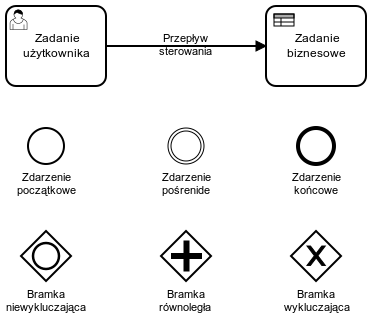
\includegraphics[width=0.6\textwidth, height=0.4\textheight,keepaspectratio]{./assets/bpmnElements.png}
    \caption{Graficzna reprezentacja podstawowych elementów \emph{BPMN}}
    \label{fig:bpmnElements}
\end{figure} 

Rysunek~\ref{fig:bpmnExample} pokazuje przykładowy model procesu w~notacji \emph{BPMN}. Jest on generalnie zrozumiały i~łatwy do analizowania. Ilustruje mały wycinek procesu związanego obsługą złożonego zamówienia przez klienta. Zdarzenie startowe rozpoczyna cały proces. Następnie wykonywane są po kolei dwa zadania. W zależności od danych, które dostarczą te elementy, bramka wykluczająca rozdziela przepływ na dwa. Przepływ górny posiada jedno zadanie, natomiast na przepływie dolnym znowu dochodzi do podziału, tym razem za pomocą bramki równoległej, gdzie wszystkie następujące elementy są wykonywane równolegle. Finalnie przepływy łączą się i~proces jest zakończony przez zdarzenie końcowe. 
\begin{figure}
    \centering
    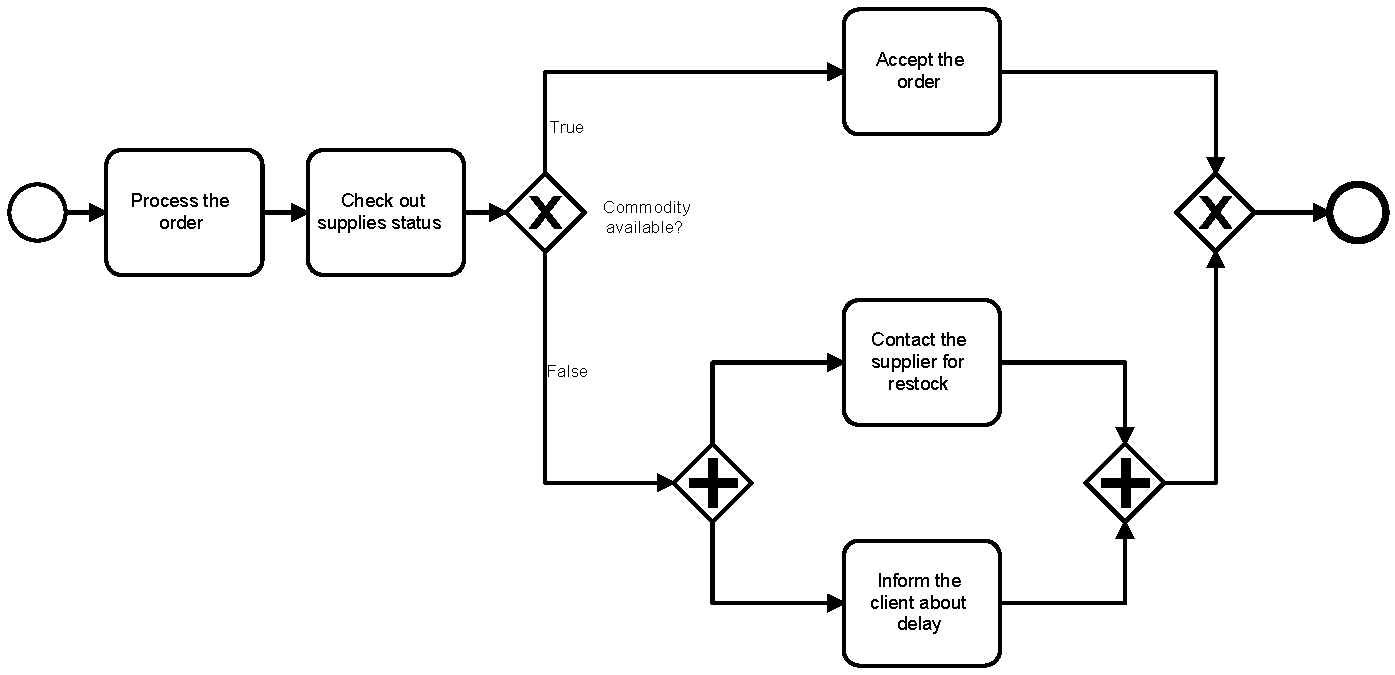
\includegraphics[width=\textwidth]{./assets/processExample.pdf}
    \caption{Przykładowy proces \emph{BPMN}}
    \label{fig:bpmnExample}
\end{figure}

%---------------------------------------------------------------------------
\section{Decision Model and Notation}
\label{sec:dmn}
\emph{DMN} (\emph{Decision Model and Notation}) jest notacją stworzoną przez OMG w~celu prostego opisu oraz modelowania reguł występujących w~procesach i~organizacjach. Tak samo jak w~przypadku \emph{BPMN} główną zaletą oraz założeniem tego standardu było umożliwienie prostej komunikacji użytkowników z~dziedzin biznesu oraz IT. Dzięki niemu bezproblemowa staje się współpraca pomiędzy ludźmi biznesu monitorującymi i~zarządzającymi decyzjami, analitykami biznesowymi, którzy szkicują wstępne wymagania decyzyjne wraz z~logiką decyzyjną oraz technicznymi programistami odpowiedzialnymi za implementację systemów, które te decyzje podejmują. Standard ten może być używany jako samodzielny, jednak najczęściej towarzyszy on notacji \emph{BPMN}. \emph{BPMN} definiuje zadanie regułowe, które może być połączone z~odpowiednim obiektem w~notacji \emph{DMN}. Dzięki temu reguły biznesowe mogą być wcielone do wykonywalnych procesów i~wraz z~działaniem przetwarzać dane oraz odpowiednio ewaluować decyzje.

\emph{DMN 1.2}~\cite{DMN12} jest w~tym momencie najnowszą wersją notacji i~definiuje on cztery elementy:
\begin{itemize}
    \item \textbf{Diagram wymagań decyzyjnych} -- diagram pokazujący zależności między elementami w~notacji \emph{DMN}. Określa on wymagania dla logiki decyzyjnej.
    \item \textbf{Kontekst biznesowy} -- kontekst decyzji, np. jak duży wpływ mają decyzje na wskaźniki wydajności lub jaka jest ich rola.
    \item \textbf{FEEL (\emph{Friendly Enough Expression Language})} -- język służący do określania reguł biznesowych w~tabelach decyzyjnych lub innych logicznych formatach.
    \item \textbf{Logika decyzyjna} -- logika będąca wewnątrz obiektów występujących w~\emph{diagramie wymagań decyzyjnych}. W kontekście tej pracy głównie będzie się to odnosić do tabel decyzyjnych.
\end{itemize}

Diagram wymagań decyzyjnych jest zbudowany bardzo podobnie do diagramu w~notacji \emph{BPMN}. Podstawowe obiekty, z~których się składa opisane zostały poniżej~\cite{DMNArticle}, natomiast rysunek~\ref{fig:dmnElements} przedstawia ich graficzną reprezentację:
\begin{itemize}
    \item \textbf{Elementy}
        \begin{itemize}
            \item \textbf{Decyzje} -- elementy determinujące wynik na podstawie pewnej ilości danych poprzez aplikowanie logiki decyzyjnej. 
            \item \textbf{Dane wejściowe} -- zewnętrzne dane, niepochodzące z~\emph{kontekstu biznesowego}. 
            \item \textbf{Źródła wiedzy} -- źródła określające reguły podejmowania decyzji. Przykładem może być tutaj polityka firmy lub regulacja.
            \item \textbf{Wiedza biznesowa} -- pewne funkcje, które enkapsulują logikę decyzyjną (reguły biznesowe, tablice decyzyjne). Powinny one być łatwe do wielokrotnego użycia.
        \end{itemize}
    \item \textbf{Wymagania}
        \begin{itemize}
            \item \textbf{Wymagania dotyczące informacji} -- połączenia wskazujące dane wejściowe oraz decyzje.
            \item \textbf{Wymagania dotyczące wiedzy} -- połączenia wskazujące jaki model wiedzy biznesowej będzie wykorzystywany w~procesie podejmowania decyzji.
            \item \textbf{Umocowanie wymagania} -- połączenia wskazujące, które z~elementów są źródłami wiedzy.
        \end{itemize}
\end{itemize}
\begin{figure}
    \centering
    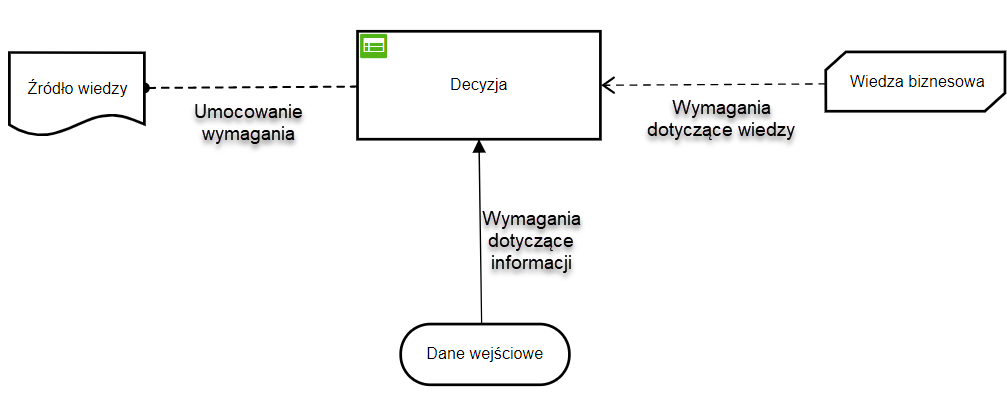
\includegraphics[width=\textwidth,height=0.4\textheight,keepaspectratio]{./assets/dmnElements2.png}
    \caption{Graficzna reprezentacja elementów \emph{diagramu wymagań decyzyjnych}}
    \label{fig:dmnElements}
\end{figure}

Rysunek~\ref{fig:dmnTable} opisuje przykładową tablicę decyzyjną. Warto zauważyć użycie \emph{FEEL} -- przykładowo~w~kolumnie OrderSize można~w~prosty sposób uzależnić zwracaną wartość od tego, czy dostarczone dane będą mniejsze lub większe od liczby dziesięć.
\begin{figure}
    \centering
    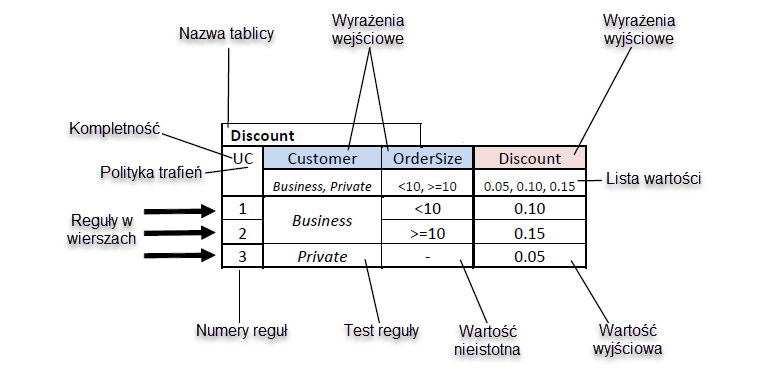
\includegraphics[width=\textwidth]{./assets/dmnTable.png}
    \caption{Tablica decyzyjna w~notacji \emph{DMN}~\cite{DMNTable}}
    \label{fig:dmnTable}
\end{figure}

Rysunek~\ref{fig:dmnExample} prezentuje jak w~praktyce wygląda integracja opisanych standardów. Zadanie regułowe w~procesie zbudowanym za pomocą notacji \emph{BPMN} jest połączone z~decyzją w~notacji \emph{DMN}. Ta z~kolei posiada pewną logikę -- reguły biznesowe wyrażone za pomocą tabeli decyzyjnej i~na tej podstawie, podczas działania procesu, ewaluuje decyzję. 
\begin{figure}
    \centering
    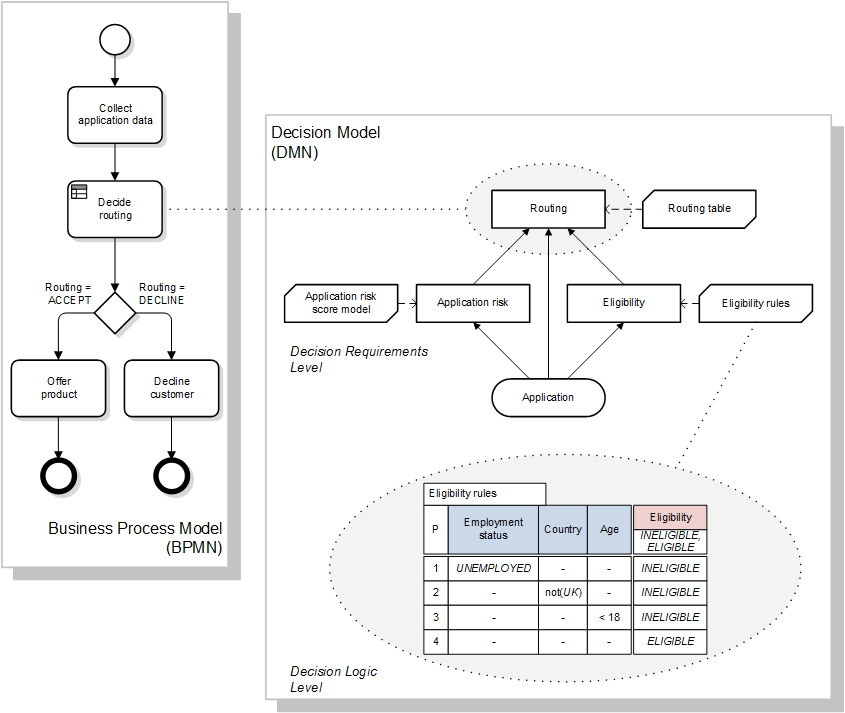
\includegraphics[width=\textwidth,height=0.4\textheight,keepaspectratio]{./assets/dmnExample.png}
    \caption{Integracja modelu \emph{BPMN} oraz \emph{DMN}~\cite{DMN12}}
    \label{fig:dmnExample}
\end{figure}

%---------------------------------------------------------------------------
\section{Attribute Relationship Diagrams}
\label{sec:ard}
\emph{ARD} (\emph{Attribute Relationship Diagrams}) to metoda, której celem jest przedstawienie relacji pomiędzy pewnymi atrybutami danego systemu. Wspomniane atrybuty są elementami branymi pod uwagę w~przypadku rozważania logiki biznesowej. Z początku metoda \emph{ARD} była zaproponowana jako mechanizm prototypowania baz wiedzy, głównie wykorzystywanych w~silnikach regułowych~\cite{ARDFirst}. Działanie miało być podobne do generowania struktur relacyjnych baz danych na podstawie diagramów ER\footnote{Więcej na temat \emph{ERD}: \url{http://citeseerx.ist.psu.edu/viewdoc/download?doi=10.1.1.526.369&rep=rep1&type=pdf}.} (\emph{Entity-Relationship Diagrams}). W kontekście tej pracy \emph{ARD} jest odpowiedzią na problem związany z~prototypowaniem modeli procesów biznesowych. Oferuje ona prosty sposób na szybkie tworzenie szkiców, z~których następnie system potrafi stworzyć bardziej skomplikowane struktury w~notacjach \emph{BPMN} oraz \emph{DMN}. Proces tworzenia modelu \emph{ARD} jest prosty i~iteracyjny, co przyczynia się do zwiększania szczegółowości modelu z~każdym kolejnym krokiem. Całość opiera się na przechodzeniu od ogólnej koncepcji do bardzo szczegółowego modelu\footnote{Rozumowanie dedukcyjne -- ,,od ogółu do szczegółu''.}, jednocześnie zachowując funkcjonalne zależności pomiędzy poszczególnymi elementami.

Diagram \emph{ARD} jest zbiorem pewnych własności i~zależności między nimi. Elementy, z~których jest zbudowany to:
\begin{itemize}
    \item \textbf{Własność} -- własność, która reprezentuje pewne atrybuty. Własności można podzielić na proste i~złożone. Każda zależność może być zależna (zależeć od innej własności) lub niezależna.
        \begin{itemize}
            \item \textbf{Prosta} -- własność prosta reprezentuje jeden atrybut. Takiej własności nie da się podzielić na pewien zbiór własności, jest atomiczna. Przykładem takiej własności może być wiek lub wzrost, są to własności reprezentujące dokładnie jeden atrybut.
            \item \textbf{Złożona} -- własność złożona, reprezentuje zbiór atrybutów. Da się ją podzielić na zbiór prostych własności. Przykładem takiej własności mogą być ,,pomiary'' -- jest to własność, która wewnątrz może kryć wiele atrybutów, takich jak np. wzrost, waga.  
        \end{itemize} 
    \item \textbf{Zależność} -- zależność łączy ze sobą własności i~pokazuje relację między nimi. 
\end{itemize}

Rysunek~\ref{fig:ardExample} prezentuję prosty diagram \emph{ARD}. Występują na nim dwie własności. ,,Pomiary'' jest własnością niezależną. Możliwym byłoby zastąpienie jej wartościami typu waga oraz wzrost. ,,Wartość BMI'' jest własnością zależną, więc nie jest możliwe ewaluowanie jej bez poprzedniego określenia własności źródłowych.
\begin{figure}
    \centering
    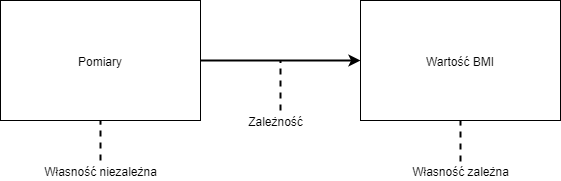
\includegraphics[width=0.6\textwidth]{./assets/ardExample.png}
    \caption{Przykład prostego diagramu \emph{ARD}}
    \label{fig:ardExample}
\end{figure}

Jasno widać, że nietrudnym zadaniem byłoby rozbudowanie takiego diagramu o kolejne własności\linebreak i~to jest główną zaletą tej metody -- prostota i~iteracyjna natura. Aby lepiej zobrazować proces tworzenia diagramu \emph{ARD} warto pochylić się nad konkretnym przykładem, wykorzystując jednocześnie diagram z~rysunku~\ref{fig:ardExample}. Niech przykładową sytuacją będzie potrzeba naszkicowania, przez analityka biznesowego, prototypu modelu związanego z~poradami zdrowotnymi. Model ma opierać się na BMI (\emph{Body Mass Index\footnote{Więcej na temat \emph{BMI}: \url{https://www.researchgate.net/publication/276444598_Body_Mass_Index}.}}). Wykorzystując wcześniej wspomniany iteracyjny proces, finalną własnością byłaby porada zdrowotna i~z~każdą kolejną iteracją analityk wprowadzałby coraz to nowsze i~bardziej szczegółowe własności, budując w~taki sposób diagram zależności. Porada potrzebowałaby imienia pacjenta oraz jego poziomu \emph{BMI}. Do obliczenia poziomu \emph{BMI} potrzebna by była płeć pacjenta oraz wartość \emph{BMI}. Natomiast sama wartość byłaby obliczana na podstawie wagi oraz wzrostu. Finalny wykres i~opisane rozumowanie obrazuje rysunek~\ref{fig:ardComplexExample}.
\begin{figure}
    \centering
    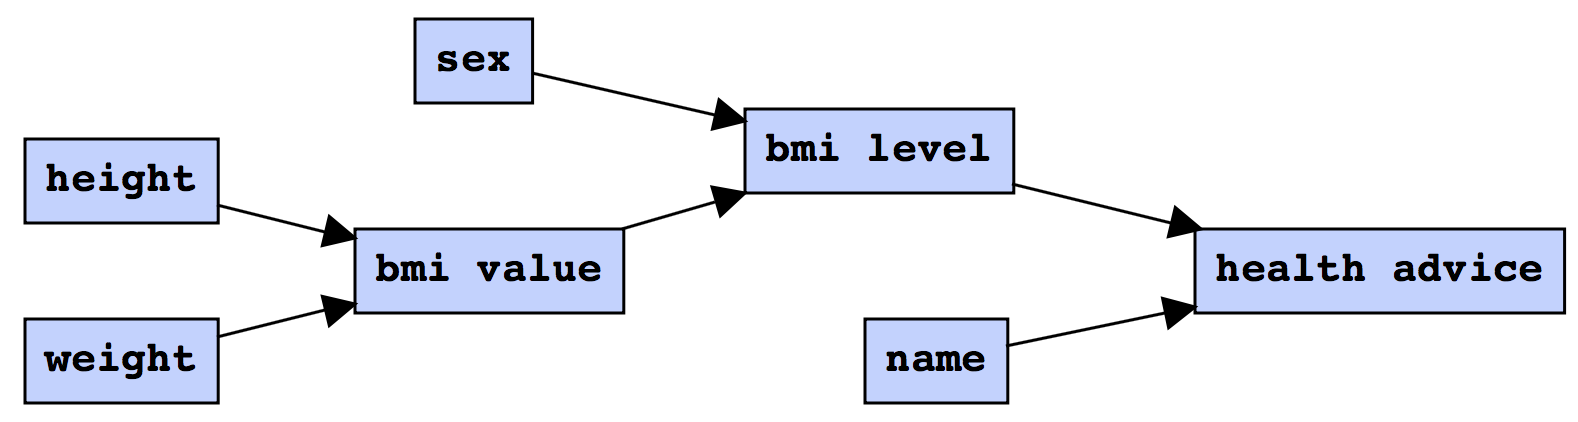
\includegraphics[width=\textwidth]{./assets/ardComplexExample.png}
    \caption{Diagram \emph{ARD} dla modelu związanego z~poradą zdrowotną~\cite{ARDtoBPM}}
    \label{fig:ardComplexExample}
\end{figure}

Wykorzystując dalej przykład z~rysunku~\ref{fig:ardComplexExample} oraz mając na uwadze wcześniej opisane standardy \emph{BPMN} oraz \emph{DMN}, można pokusić się o przeniesienie tego prototypu do wspomnianych notacji. Rysunek~\ref{fig:ardBPMDMNFinal} prezentuje koncepcję takiej operacji. Wystarczyłoby odpowiednio pogrupować własności i~ich zależności, przedstawić każdą własność prostą jako zadnie użytkownika, w~którym użytkownik musi podać dane, a~każdą własność złożoną jako zadanie biznesowe, czyli zadanie połączone z~decyzją (gdzie wykorzystywana jest tablica decyzyjna). Na wspomnianym rysunku przykładem zadania użytkownika jest ,,Enter Measures'', które dostarcza ,,height'' oraz ,,width'' do tablic decyzyjnych, a~przykładem zadania biznesowego jest ,,Determine bmi level''.
\begin{figure}
    \centering
    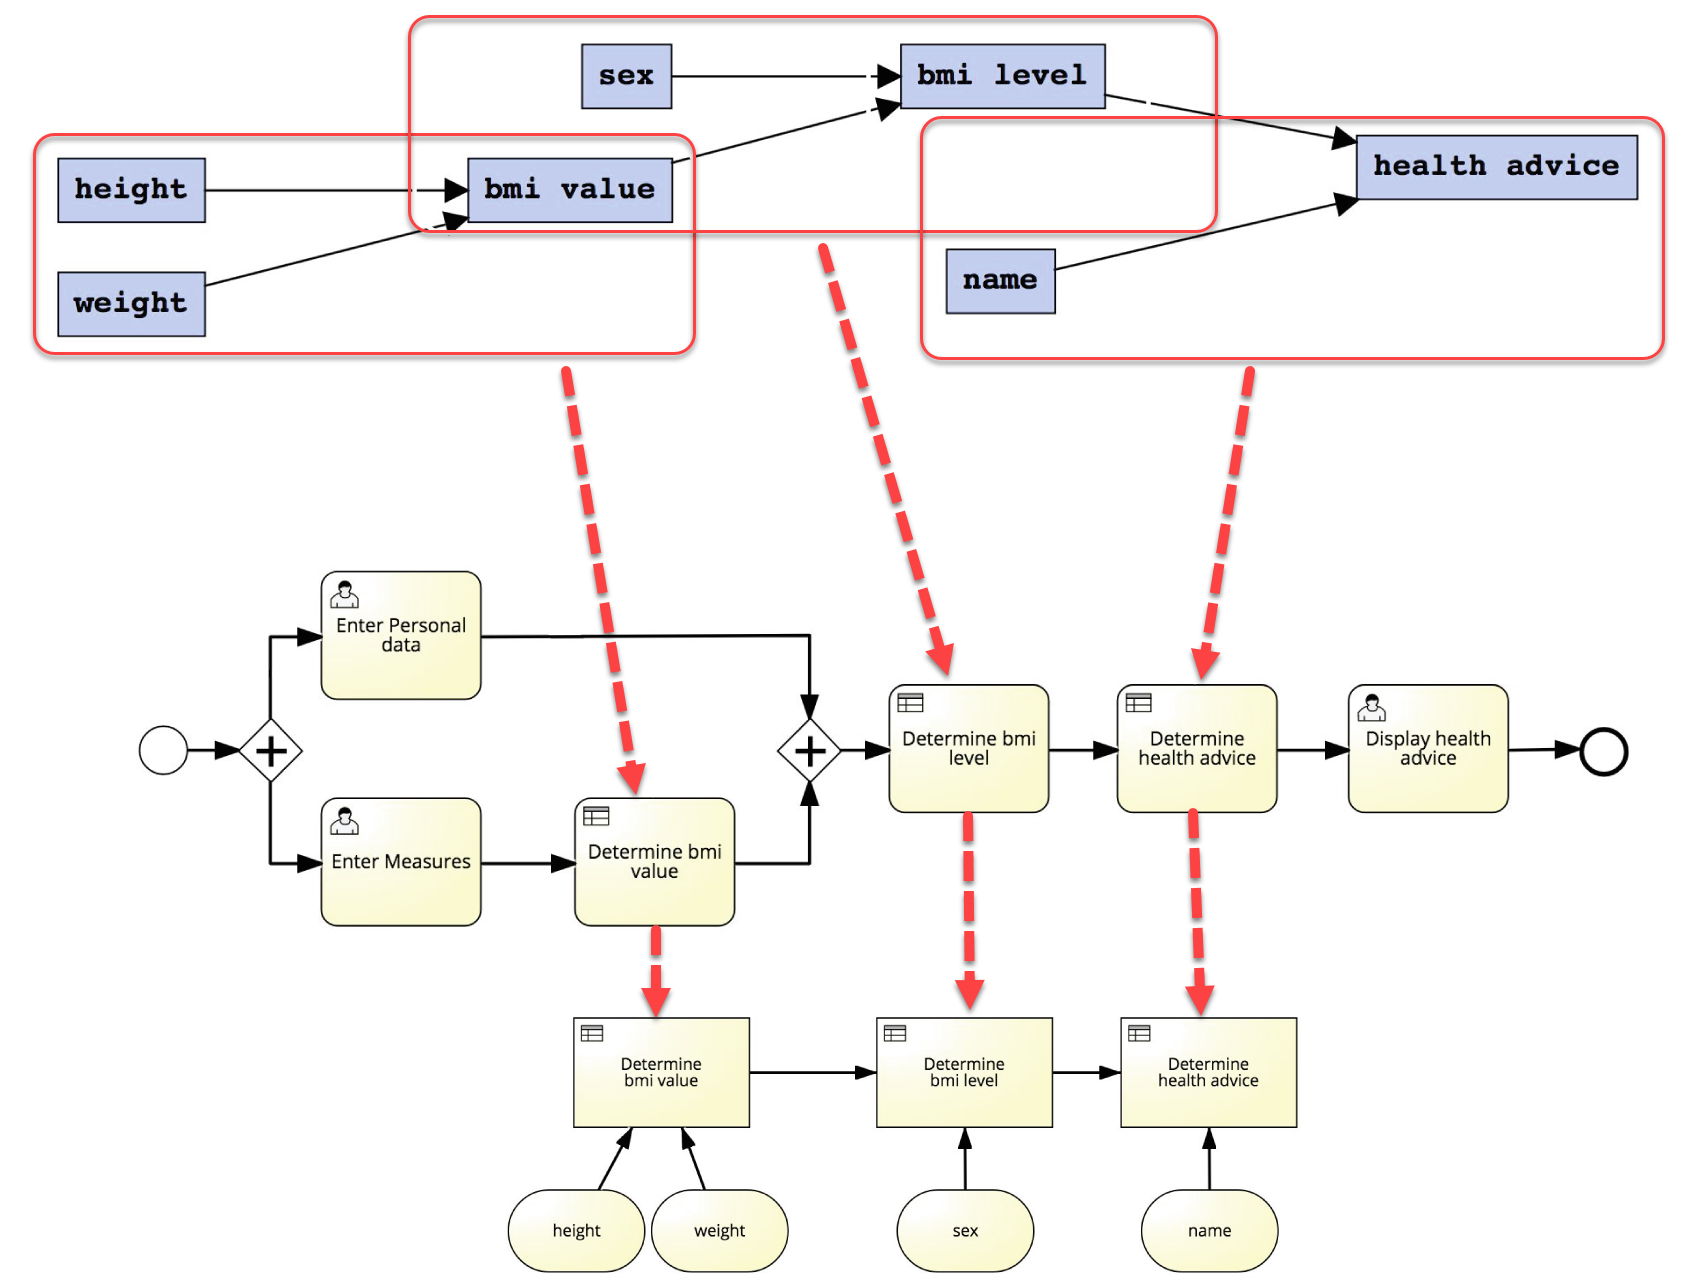
\includegraphics[width=\textwidth,height=0.4\textheight,keepaspectratio]{./assets/ardBPMDMNFinal.png}
    \caption{Koncept transformacji diagramu \emph{ARD} do modelu w~notacji \emph{BPMN} oraz \emph{DMN}~\cite{ARDtoBPM}}
    \label{fig:ardBPMDMNFinal}
\end{figure} 

%---------------------------------------------------------------------------
\subsection{Hekate Markup Langauge}
\label{sec:hml}
\emph{HML} (\emph{Hekate Markup Language}) to język stworzony do reprezentacji bazy reguł \emph{HeKatE\footnote{Więcej na temat \emph{HeKatE}: \url{https://ai.ia.agh.edu.pl/hekate:start}.}}, zapisanych formacie HMR (\emph{Hekate Meta Representation\footnote{Więcej na temat \emph{HMR}: \url{https://ai.ia.agh.edu.pl/hekate:hmr}.}}). Język \emph{HML} posiada trzy podzbiory:
\begin{itemize}
    \item \textbf{attml} -- Attribute Markup Language opisujący atrybuty reguł,
    \item \textbf{ardml} -- Attribute Relationship Markup Language służący do ekspresji prototypów w~ARDplus (rozszerzeniu \emph{ARD}),
    \item \textbf{xttml} -- XTT2 Rule Markup Language służący do reprezentacji ustrukturyzowanych reguł XTT2\footnote{Więcej na temat \emph{XTT2}: \url{https://ai.ia.agh.edu.pl/hekate:xtt2}.}.
\end{itemize}
W zależności od potrzeb, możliwe jest różnorakie wykorzystanie opisanych podjęzyków:
\begin{itemize}
    \item \textbf{attml} -- tylko definicje atrybutów (minimalistyczny przypadek),
    \item \textbf{attml + ardml} -- atrybuty oraz zależności \emph{ARD}, 
    \item \textbf{attml + ardml + xttml} -- atrybuty, zależności oraz reguły \emph{XTT2},
    \item \textbf{attml + xttml} -- atrybuty i~reguły (bez prototypu \emph{ARD}).
\end{itemize}\newpage
Listing~\ref{lst:hmlFileExample} prezentuje strukturę pliku \emph{HML} wykorzystującego wszystkie wspomniane podjęzyki. 
\lstinputlisting[language=XML, caption={Przykład struktury pełnego pliku \emph{HML}}, label={lst:hmlFileExample}]{./listings/hmlFileExample.xml}

Składnia wymaga, aby wszystkie ważne elementy posiadały atrybut ,,id'', będący unikatowym identyfikatorem. Dodatkowo każdy element powinien zawierać odpowiedni przedrostek:
\begin{itemize}
    \item \texttt{types} -- identyfikator powinien zaczynać się od ,,tpe'',
    \item \texttt{attributes} -- identyfikator powinien zaczynać się od ,,att'',
    \item \texttt{properties} -- identyfikator powinien zaczynać się od ,,prp'',
    \item \texttt{type groups} -- identyfikator powinien zaczynać się od ,,tgr'',
    \item \texttt{attribute groups} -- identyfikator powinien zaczynać się od ,,agr'',
    \item \texttt{dependencies} -- identyfikator powinien zaczynać się od ,,dep'',
    \item \texttt{ARD history} -- identyfikator powinien zaczynać się od ,,hst''.
\end{itemize}

W kontekście niniejszej pracy pliki \emph{HML}, które będą brane pod uwagę, powinny zawierać w~sobie podzbiór językowy \emph{ardml}, jednak z~opcjonalnym fragmentem \emph{TPH}, gdyż nie jest on wykorzystywany przy tworzeniu modelu procesu finalnego. Przykład wymaganego pliku prezentuje listing~\ref{lst:ardmlExample}.
\lstinputlisting[language=XML, caption={Przykład struktury pliku \emph{HML} z~podzbiorem \emph{ardml}}, label={lst:ardmlExample}]{./listings/ardmlExample.xml}
\vspace{1cm}

Jest to koniec rozdziału opisującego metody reprezentacji procesów i~decyzji. W tym rozdziale opisane zostały najważniejsze terminy, które będą często pojawiać się w~dalszej części niniejszej pracy. W~kolejnym rozdziale zostanie przedstawiony projekt aplikacji, która wykorzystuje opisane tutaj notacje \emph{BPMN}, \emph{DMN} oraz \emph{ARD}.


\chapter{Projekt aplikacji}
\label{cha:projektAplikacji}
Rozdział opisuje architekturę systemu w~ujęciu abstrakcyjnym. Nacisk położony jest na schemat działania oraz przedstawienie komponentów aplikacji. Dodatkowo wyjaśniane są pewne podstawowe pojęcia związane z~inżynierią oprogramowania.

%---------------------------------------------------------------------------
\section{Podstawowe przypadki użycia}
\label{sec:podstawowePrzypadkiUżycia}
Aplikacja ,,DAR'' jest z~punktu widzenia funkcjonalności dość prostym systemem. Rysunek~\ref{fig:usecase} prezentuje podstawowe przypadki użycia -- warto mieć jednak na uwadze fakt, że aplikacja została zintegrowana z~zewnętrznym systemem posiadającym silniki decyzyjne i~procesowe, zatem wiele funkcjonalności niepokazanych tutaj, takich jak uruchamianie procesu, ewaluacja decyzji czy monitorowanie wydajności procesów, leży po jego stronie.
\begin{figure}
    \centering
    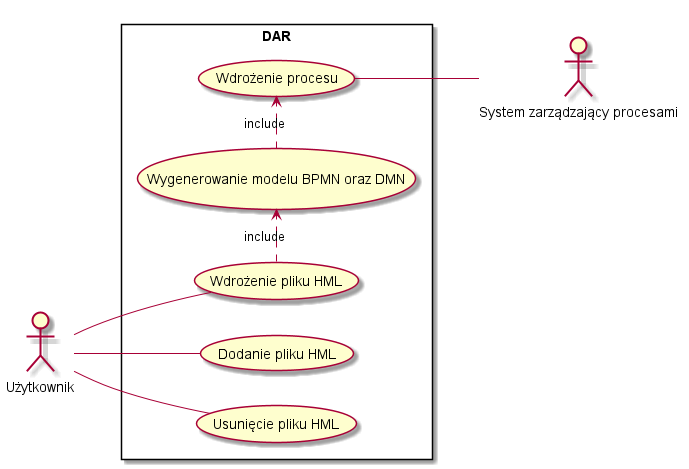
\includegraphics[width=\textwidth, height=0.4\textheight,keepaspectratio]{./assets/usecase.png}
    \caption{Graficzna reprezentacja podstawowych przypadków użycia}
    \label{fig:usecase}
\end{figure} 

Poniżej opisane zostały funkcjonalności zaprezentowane na rysunku~\ref{fig:usecase}:
\begin{itemize}
	\item \textbf{Wdrożenie procesu} -- aplikacja przesyła dwa pliki do zewnętrznego systemu. Pierwszy z~nich to plik reprezentujący proces w~notacji \emph{BPMN}, natomiast drugi to plik reprezentujący diagram decyzji w~notacji \emph{DMN}.
	\item \textbf{Wygenerowanie modelu BPMN oraz DMN} -- aplikacja na podstawie dostarczonych danych generuje dwa modele -- model w~notacji \emph{BPMN} oraz model w~notacji \emph{DMN}. Jednocześnie spaja te dwa modele poprzez odpowiednie ustawienia atrybutów.
	\item \textbf{Wdrożenie pliku HML} -- aplikacja przesyła wybrany plik \emph{HML} i~rozpoczyna proces jego przetwarzania aby finalnie przesłać go do odrębnego systemu procesowego. 
    \item \textbf{Dodanie pliku HML} -- aplikacja zapisuje informację z~plików \emph{HML}.
    \item \textbf{Usunięcie pliku HML} -- aplikacja usuwa wszystkie zapisane informacje z~danego pliku \emph{HML}.
    \item \textbf{Uruchamianie procesu, ewaluacja decyzji, monitorowanie procesu...} -- wiele funkcjonalności nie należy stricte do ram aplikacji ,,DAR'', jednak poprzez integrację z~zewnętrznym systemem, aplikacja pośredniczy w~umożliwianiu takich działań, jak uruchamianie i~śledzenie procesu, edycja tabel decyzyjnych, uzupełnianie danych czy ewaluacja decyzji. 
\end{itemize}

%---------------------------------------------------------------------------
\section{Architektura systemu}
\label{sec:architekturaSystemu}

%---------------------------------------------------------------------------
\subsection{Architektura N-tier}
\label{sec:architekturaNTier}
Aplikacja ,,DAR'' została oparta na architekturze wielowarstwowej zwanej również architekturą N-tier. Jest to jedna z metod tworzenia oprogramowania, opierająca się na wydzieleniu warstw aplikacji -- w~sensie fizycznym oraz logicznym. Warstwy są narzędziem do odseparowania obowiązków\footnote{Jest to ściśle związane z~zasadą SoC (\emph{Separation of Concerns}), czyli podstawową zasadą inżynierii oprogramowania, stanowiącą o tym, że każda część systemu powinna mieć silnie określone granice i~adresować dokładnie odseparowaną kwestię.} danych rejonów aplikacji oraz do zarządzania zależnościami. Każda warstwa posiada konkretną odpowiedzialność. Warstwy wyższe mogą używać usług z~warstw niższych, jednak nie działa to w~drugą stronę. Architektura wielowarstwowa może być:
\begin{itemize}
    \item \textbf{Zamknięta} -- tak jak jest to w~przypadku opisywanego systemu. Dana warstwa może używać jedynie warstwy pod sobą.
    \item \textbf{Otwarta} -- dana warstwa może używać dowolnej warstwy pod sobą.
\end{itemize}

,,DAR'' posiada trzy logiczne warstwy, zaprezentowane na rysunku~\ref{fig:layerExample}.
\begin{figure}
    \centering
    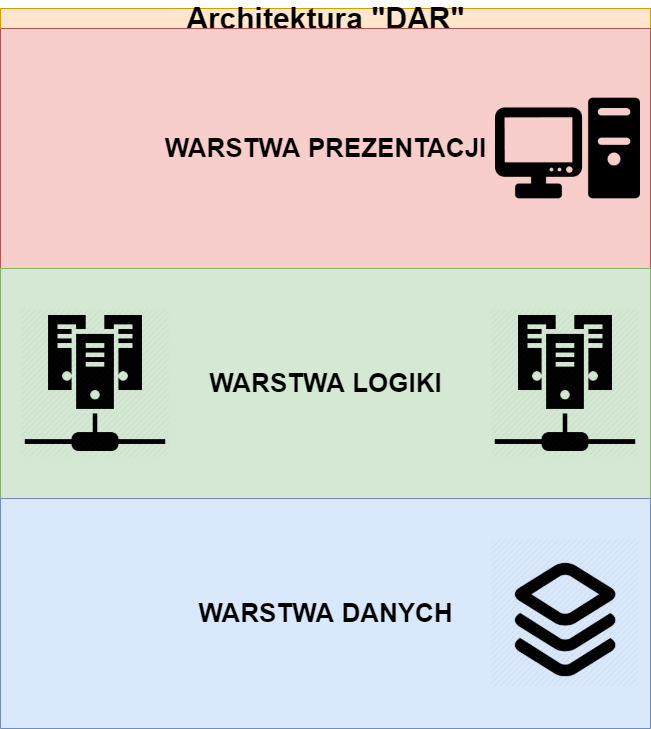
\includegraphics[width=0.4\textwidth,height=0.4\textheight,keepaspectratio]{./assets/layerExample.png}
    \caption{Warstwy aplikacji ,,DAR''}
    \label{fig:layerExample}
\end{figure} 
Poniżej przedstawiony został opis wydzielonych warstw:
\begin{itemize}
    \item \textbf{Warstwa prezentacji} -- najwyższa warstwa. Jej zadaniem jest wyświetlanie danych i~komunikacja z~warstwą niżej. Reprezentuje ona interfejs użytkownika i umożliwia interakcję z~systemem.
    \item \textbf{Warstwa logiki} -- zwana również logiką biznesową, jest to główna część aplikacji, w~której zaimplementowane zostały wszystkie funkcjonalności. W przypadku ,,DAR'' do dyspozycji są tutaj dwa serwisy, jeden będący serwerem ,,DAR'', natomiast drugi to zintegrowany zewnętrzny system do obsługi procesów. Warstwa ta przetwarza dane i~przekazuje je do warstwy prezentacji. 
    \item \textbf{Warstwa danych} -- warstwa związana z~dostępem do danych. W~przypadku ,,DAR'' jest to dostęp do relacyjnej bazy danych, gdzie przechowywane są informacje na temat dodanych plików \emph{HML}. Udostępnia ona dane dla warstwy logiki biznesowej.
\end{itemize}
Zaletami takiego rozwiązania są:
\begin{itemize}
    \item \textbf{Skalowalność} -- dzięki oddzieleniu odpowiedzialności bardzo łatwo zdiagnozować, gdzie aplikacja potrzebuje usprawnień i~co najważniejsze, można to robić tylko w~jednym konkretnym obszarze, co daje o wiele więcej możliwości skalowania.
    \vspace{-1mm}
    \item \textbf{Luźne powiązania} -- architektura wymusza na programiście ograniczenie zależności, dzięki czemu zmiany w~danej warstwie są bezbolesne z~punktu widzenia innych warstw.
    \vspace{-1mm} 
    \item \textbf{Bezpieczeństwo} -- podział na warstwy niesie też ze sobą więcej możliwości ochrony przed atakami, ponieważ w~każdej warstwie może występować inna metoda ochrony. Dodatkowo tak samo jak w~przypadku skalowania można odpowiednio poświęcić środki na ochronę tylko newralgicznych punktów aplikacji (przykładem może być zwiększona ochrona warstwy logiki biznesowej oraz danych niż warstwy prezentacji).
    \vspace{-1mm}
    \item \textbf{Łatwiejszy proces tworzenia aplikacji} -- każdą warstwą może zajmować się inna osoba lub zespół, ze względu na luźne powiązania.
    \vspace{-1mm}
    \item \textbf{Większy nacisk na powtórne użycie} -- dzięki modularności tego podejścia, komponenty są raczej projektowane w~sposób generyczny, co ułatwia ich ponowne użycie.
\end{itemize}

%---------------------------------------------------------------------------
\subsection{Architektura klient-serwer}
\label{sec:architekturaKlientSerwer}
,,DAR'' jest aplikacją internetową działająca na zasadzie klient-serwer. Jest to metoda działania, która opiera się na podzieleniu aplikacji na dwie części i~na komunikacji tych modułów:
\begin{itemize}
    \item \textbf{Front-end} -- część kliencka, działająca na oprogramowaniu klienckim, w~tym przypadku jest to przeglądarka użytkownika. Ta część reprezentuje interfejs użytkownika. W aplikacji ,,DAR'' \emph{front-end} został zrealizowany w~formie SPA (\emph{Single Page Application}\footnote{Więcej na temat \emph{SPA} w~rozdziale \ref{sec:spa}.}). Do tej części należy \emph{warstwa prezentacji} opisywana wcześniej.
    \item \textbf{Back-end} --  część serwerowa, działająca na osobnym serwerze. Do niej należą \emph{warstwa logiki biznesowej} oraz \emph{warstwa danych}  opisane wcześniej. W przypadku systemu ,,DAR'' została zrealizowana za pomocą internetowego \emph{REST}\footnote{Więcej na temat protokołu \emph{REST} w~rozdziale \ref{sec:rest}.} API (\emph{Application Programming Interface}). 
\end{itemize}
 W opisywanej aplikacji klient wysyła zapytanie \emph{HTTP}\footnote{Więcej na temat protokołu \emph{HTTP} w~rozdziale \ref{sec:http}.} przez sieć internetową do serwera, a~ten przetwarza żądanie i~zwraca odpowiedź, często z~towarzyszącymi temu danymi. Komunikacja jest asynchroniczna, dzięki temu zwiększona jest odczuwalna szybkość działania aplikacji.

%---------------------------------------------------------------------------
\subsubsection{Protokół HTTP}
\label{sec:http}
Protokół \emph{HTTP} (\emph{Hypertext Transfer Protocol}) to bezstanowy protokół do przesyłania dokumentów typu hypermedia. Określa on zasady wymiany informacji, normalizuje i~ujednolica sposoby komunikacji pomiędzy urządzeniami. Jego głównym zastosowaniem jest umożliwienie komunikacji pomiędzy aplikacjami internetowymi (przeglądarkami), a~serwerami (komputerami/chmurą). Wymiana informacji przebiega w~następujący sposób:
\begin{itemize}
    \item Klient (przeglądarka) wysyła zapytanie \emph{HTTP} do sieci.
    \item Serwer internetowy otrzymuje zapytanie.
    \item Serwer uruchamia aplikację, aby przetworzyć zapytanie.
    \item Serwer zwraca odpowiedź \emph{HTTP} to przeglądarki.\
    \item Klient otrzymuje odpowiedź.
\end{itemize}
Rysunek~\ref{fig:httpExample} obrazuje wymianę informacji w~protokole \emph{HTTP} pomiędzy klientem a~serwerem,.
\begin{figure}
    \centering
    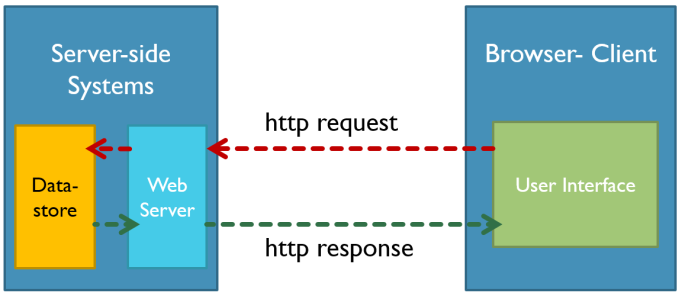
\includegraphics[width=0.5\textwidth,height=0.5\textheight,keepaspectratio]{./assets/httpRequestExample.png}
    \caption{Przykład komunikacji za pomocą protokołu \emph{HTTP}~\cite{HTTP}}
    \label{fig:httpExample}
\end{figure}

Klient, aby otrzymać odpowiedź od serwera, musi określić jego adres oraz metodę określającą jakiego typu jest zapytanie. Najważniejsze metody określone przez specyfikację \emph{HTTP}~\cite{HTTPSpecification} są następujące:
\begin{itemize}
    \item \textbf{GET} -- pobranie zasobu wskazanego za pomocą adresu.
    \item \textbf{PUT} -- wysłanie danych, najczęściej aby zaktualizować pewne istniejące już dane.
    \item \textbf{POST} -- wysłanie danych, najczęściej aby stworzyć kompletnie nowy zasób.
    \item \textbf{DELETE} -- usunięcie danych.
\end{itemize}

%---------------------------------------------------------------------------
\subsubsection{REST API}
\label{sec:rest}
REST (\emph{Representational State Transfer}) jest to styl architektury oprogramowania, bazujący na zbiorze określonych reguł, które określają, jak definiowane są zasoby, a~co za tym idzie, jak można otrzymać do nich dostęp. API (\emph{Application Programming Interface}) jest to zestaw pewnych zasad określających komunikację pomiędzy oprogramowaniem komputerowym. Innymi słowy, wiążąc te dwa pojęcia, \emph{API} to reguły określające, jakie zasoby są dostępne i~jak interesariusz może je uzyskać, natomiast \emph{REST} to styl określający schemat oraz budowę \emph{API}. Aby interfejs był w~pełni zgodny z~\emph{REST}, czyli był \emph{RESTful}, musi spełnić sześć podstawowych reguł z~nim związanych:
\begin{itemize}
    \item \textbf{Klient-serwer} -- system powinien wspierać architekturę typu klient-serwer, jest to związane z~podziałem odpowiedzialności. Odseparowując interfejs użytkownika od przechowywania danych zwiększona zostaje modularność, przez co zyskuje na tym skalowalność.
    \item \textbf{Bezstanowość} -- każda komunikacja na kanale klient-serwer jest w~pełni samowystarczalna, posiada wszelkie niezbędne informacje. Żaden kontekst klienta nie jest przechowywany na serwerze pomiędzy zapytaniami.
    \item \textbf{Zdolność wykorzystania cache'a} -- odpowiedź z~\emph{REST API} musi być jasno określona jako zdolna lub niezdolna do wykorzystania cache'a.
    \item \textbf{Zunifikowany interfejs} -- punkt końcowy, czyli adres danego zasobu powinien być jednoznaczny. Użytkownik zawsze powinien wiedzieć do jakiego zasobu się odwołuje. Polega to głównie na odpowiedniej budowie adresów.
    \item \textbf{System warstwowy} -- system powinien wprowadzać separację warstw.
    \item \textbf{Kod na żądanie} -- zasada opcjonalna polegająca na udostępnianiu klientowi apletów i~skryptów.
\end{itemize}

Główną kwestią, na którą kładzie nacisk \emph{REST} są zasoby. Każda informacja, która może być nazwana, może być zasobem. Zasób jest to obiekt z~typem, danymi, relacjami do innych zasobów oraz z~zestawem metod pozwalających na nim operować. Można go przyrównać do obiektu w~programowaniu obiektowym. Zasoby mogą być oczywiście grupowane w~kolekcję. Stan danego zasobu w~dowolnym czasie jest znany jako reprezentacja zasobu. Zawiera ona dane, metadane opisujące zasób oraz linki typu hypermedia, które pomagają w~podejmowaniu kolejnych akcji. Jeśli chodzi o same dane, które zawiera reprezentacja, przeważnie reprezentowane są one w~formacie \emph{JSON}\footnote{Więcej na temat \emph{JSON}: \url{https://www.json.org/json-en.html}.} (jednak występuje tutaj pełna dowolność, nic nie stoi na przeszkodzie, aby użyć formatu \emph{XML}). 

Mówiąc o metodach, które zasób udostępnia, należy wrócić do wcześniej opisanego protokołu \emph{HTTP}, ponieważ to właśnie tego protokołu używa \emph{REST} do komunikacji. Konsumenci \emph{API} uzyskują dostęp do zasobów poprzez wykorzystanie odpowiedniego internetowego adresu \emph{URI} (\emph{Uniform Resource Identifier}\footnote{Więcej na temat \emph{URI}: \url{https://www.w3.org/Addressing/URL/uri-spec.html}.}) oraz odpowiedniej metody \emph{HTTP}. Innymi słowy komunikacja opiera się na wysyłaniu zapytania \emph{HTTP} z~określoną metodą, pod odpowiedni adres i~otrzymaniu odpowiedzi \emph{HTTP} z~określonym rezultatem i~towarzyszącą mu reprezentacją zasobu. Głównie wykorzystywane są cztery metody, przez co wiele prostych aplikacji będących \emph{RESTful} jest nazywanych aplikacjami \emph{CRUD} -- rysunek~\ref{fig:crudExample} tłumaczy znaczenie tego terminu i~przedstawia wspomniane metody. 
\begin{figure}
    \centering
    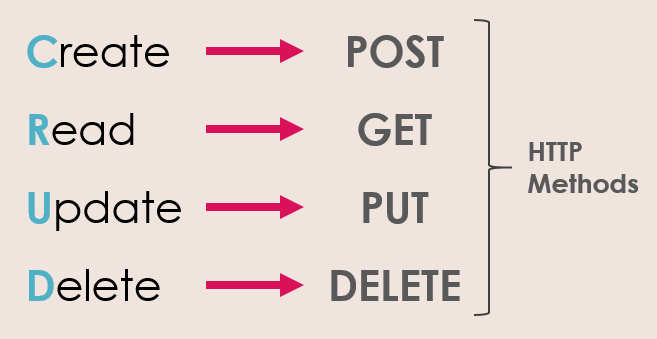
\includegraphics[width=0.5\textwidth,height=0.5\textheight,keepaspectratio]{./assets/crudExample.png}
    \caption{Główne metody wykorzystywane w~\emph{REST API} i~geneza terminu \emph{CRUD}~\cite{CRUD}}
    \label{fig:crudExample}
\end{figure}

%---------------------------------------------------------------------------
\subsubsection{SPA}
\label{sec:spa}
\emph{SPA} (\emph{Single Page Application}) to podejście do tworzenia klienckiego interfejsu użytkownika w~przeglądarce, a~dokładniej wcześniej wspomnianego już front-endu, bardzo mocno zyskujące na popularności w~ostatnich latach, opierające się na dynamicznym wyświetlaniu danych i~przebudowie tylko części widoku. W podejściu klasycznym czyli \emph{MPA} (\emph{Multipage Application}) za każdym razem, kiedy użytkownik nawigował się po stronie internetowej, przeglądarka wysyłała żądanie do serwera i~w~odpowiedzi otrzymywała nową stronę \emph{HTML}\footnote{Więcej na temat \emph{HTML}: \url{https://developer.mozilla.org/pl/docs/Web/HTML}.}, którą następnie wyświetlała. \emph{SPA} inaczej podchodzi do tematu nawigacji, zamiast zawsze prosić o nową stronę \emph{HTML}, cały front-end jest ładowany do przeglądarki na samym początku uruchomienia strony, a~wszelkie zapytania do serwera skutkują jedynie zwróceniem konkretnych danych (najczęściej w~formacie \emph{JSON}). Dzięki temu, to po stronie klienckiej leży odpowiedzialność za odpowiednie wyświetlanie danych. Innymi słowy nie następuje przekierowanie na kolejną stronę, wyświetlana jest cały czas tylko jedna (co zresztą sugeruje nazwa \emph{SPA}), ale to co na niej się znajduje jest dynamicznie zmieniane. 

Warstwa prezentacji w~opisywanej aplikacji została stworzona właśnie w~podejściu \emph{SPA}. Front-end komunikuje się z~serwerem za pomocą \emph{REST API}, otrzymując w~odpowiedzi dane w~formacie \emph{JSON}, a~następnie odpowiednio je przetwarza. Korzyści jakie przynosi ze sobą takie podejście są następujące:
\begin{itemize}
    \item \textbf{Wydajność} -- aplikacja jest szybsza, ponieważ o wiele mniej danych zostaje przetransportowane przez sieć internetową.
    \item \textbf{Mniejsze obciążenie serwera} -- serwer może skupić się tylko i~wyłącznie na przetwarzaniu danych, a~nie na konstrukcji widoku.
    \item \textbf{Większe możliwości prezentacji treści} -- przez brak ciągłego odświeżania strony, umożliwione są efekty, które wcześniej zarezerwowane były jedynie dla aplikacji natywnych dla urządzeń mobilnych lub desktopowych.
    \item \textbf{Zwiększenie odczuwalnej szybkości działania aplikacji} --  aplikacja sprawia wrażenie szybszej, ponieważ niepotrzebne są całościowe przeładowania strony.
\end{itemize}

%---------------------------------------------------------------------------
\section{Schemat projektu}
\label{sec:schematAplikacji}
Rysunek~\ref{fig:projectScheme} przedstawia generalny schemat projektu.
\begin{figure}
    \centering
    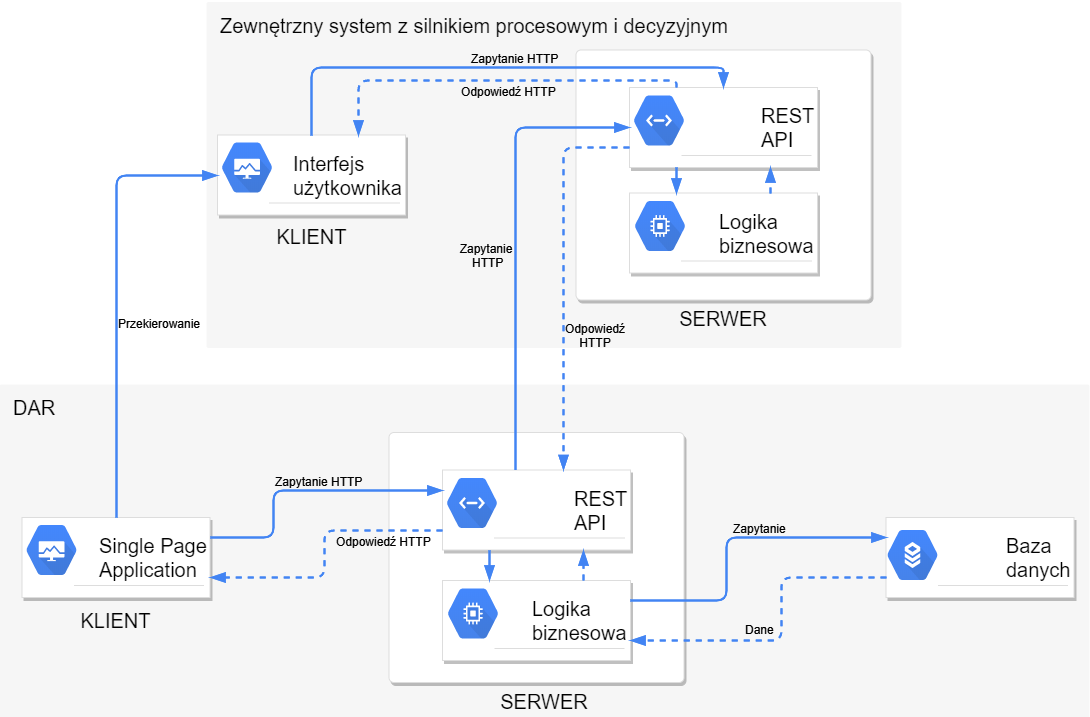
\includegraphics[width=\textwidth]{./assets/projectScheme.png}
    \caption{Schemat projektu ,,DAR''}
    \label{fig:projectScheme}
\end{figure}
Jak widać w~projekcie dochodzi do integracji dwóch systemów. ,,DAR'' udostępnia aplikację \emph{SPA} po stronie klienckiej, która komunikuje się z~serwisem za pomocą \emph{REST API}, wysyłając odpowiednie zapytanie \emph{HTTP}. Serwis po otrzymaniu żądania wykonuje zaimplementowaną logikę biznesową, korzystając przy tym z~bazy danych, aby finalnie zwrócić odpowiedź. Ma on również możliwość komunikacji z~serwisem zewnętrznego systemu, który również udostępnia \emph{REST API}. Front-end aplikacji ,,DAR'' ma możliwość przekierowania użytkownika do interfejsu wspomnianego zewnętrznego systemu. 

Podsumowując schemat projektu, występują w~nim dwa zintegrowane ze sobą serwisy, dwa interfejsy użytkownika oraz baza danych. Sercem całego projektu jest back-end aplikacji, ponieważ to on integruje ze sobą resztę modułów i~to on odpowiedzialny jest za pracę związaną z~generacją modeli procesów i~wdrażaniem ich do zewnętrznego systemu.  

%---------------------------------------------------------------------------
\section{Komponenty}
\label{sec:komponenty}
Nawiązując do rysunku~\ref{fig:projectScheme}, warto przyjrzeć się bliżej części ,,DAR''. Rysunek~\ref{fig:components} prezentuje wyodrębnione komponenty aplikacji. Należy jednak zaznaczyć, że jest to zbliżenie tylko na wspomnianą wcześniej część, nie pojawiają się tam elementy zewnętrznego systemu, z~którymi wiele z~tych komponentów jest zintegrowanych. 
\begin{figure}
    \centering
    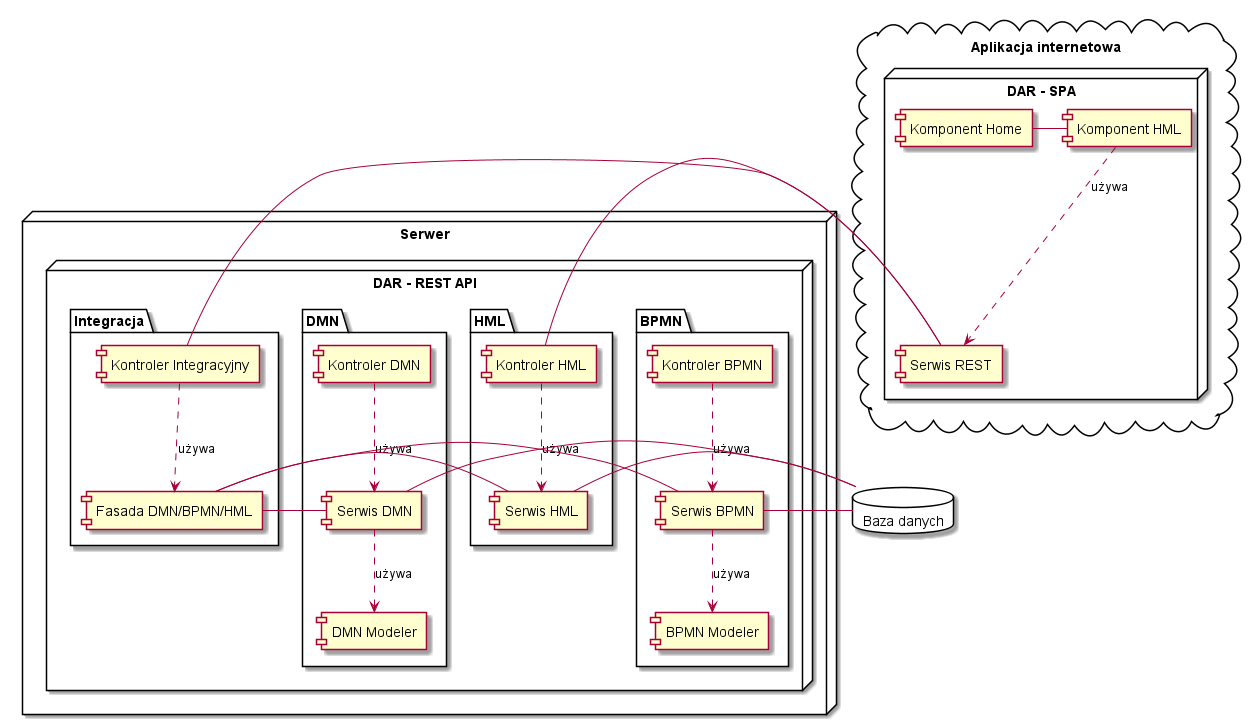
\includegraphics[width=\textwidth]{./assets/components.png}
    \caption{Komponenty aplikacji ,,DAR''}
    \label{fig:components}
\end{figure} 

Podział komponentów na załączonym rysunku jest następujący:
\begin{itemize}
    \item \textbf{Serwer} 
        \begin{itemize}
            \item \textbf{HML}
                \begin{itemize}
                    \item \textbf{Kontroler HML} -- część odpowiedzialna za komunikację \emph{HTTP} i~określająca adresy funkcjonalności związanych z~plikami \emph{HML}.
                    \item \textbf{Serwis HML} -- część odpowiedzialna za logikę biznesową związaną z~plikami \emph{HML}. Zapewnia komunikację z~bazą danych.
                \end{itemize}
            \item \textbf{BPMN}
                \begin{itemize}
                    \item \textbf{Kontroler BPMN} -- część odpowiedzialna za komunikację \emph{HTTP} i~określająca adresy funkcjonalności związanych z~modelami \emph{BPMN}.
                    \item \textbf{Serwis BPMN} -- część odpowiedzialna za logikę biznesową związaną z~modelami \emph{BPMN}. Zapewnia komunikację z~bazą danych.
                    \item \textbf{Modeler BPMN} -- część odpowiedzialna za tworzenie modeli \emph{BPMN}.
                \end{itemize}
            \item \textbf{DMN}
                \begin{itemize}
                    \item \textbf{Kontroler DMN} -- część odpowiedzialna za komunikację \emph{HTTP} i~określająca adresy funkcjonalności związanych z~modelami \emph{DMN}.
                    \item \textbf{Serwis DMN} -- część odpowiedzialna za logikę biznesową związaną z~modelami \emph{DMN}. Zapewnia komunikację z~bazą danych.
                    \item \textbf{Modeler BPMN} -- część odpowiedzialna za tworzenie modeli \emph{DMN}.
                \end{itemize}
            \item \textbf{Integracja}
                \begin{itemize}
                    \item \textbf{Kontroler integracyjny} -- nazwany integracyjnym, ponieważ jego głównym zadaniem jest integracja z~zewnętrznym systemem posiadającym silniki decyzyjne oraz procesowe i~komunikację \emph{HTTP}, określając adresy funkcjonalności związanych z~tym systemem.
                    \item \textbf{Fasada DMN/BPMN/HML} -- fasada wyżej opisanych serwisów, implementująca logikę biznesową związaną z~wdrożeniem modeli procesów do zewnętrznego systemu.
                \end{itemize}
        \end{itemize}
    \item \textbf{Aplikacja internetowa}
        \begin{itemize}
            \item \textbf{Komponent Home} -- część domyślna aplikacji klienckiej, pozwala na nawigację do kolejnych elementów.
            \item \textbf{Komponent HML} -- serce części klienckiej, gdzie znajduje się główny widok i~to on odpowiada za umożliwienie użytkownikowi podstawowych interakcji typu dodanie i~wdrożenie pliku \emph{HML}.
            \item \textbf{Serwis REST} -- serwis do komunikacji za pomocą protokołu \emph{HTTP}, wykorzystywany przez \emph{Komponent HML} do wysyłania zapytań \emph{HTTP}.
        \end{itemize} 
    \item \textbf{Baza danych} -- część odpowiedzialna za przechowywanie danych.
\end{itemize}

%---------------------------------------------------------------------------
\section{Schemat interakcji}
Rysunek~\ref{fig:sequence} prezentuje główny schemat interakcji pomiędzy komponentami na przykładzie procesu wgrywania pliku \emph{HML} przez użytkownika oraz wdrażania tego pliku do zewnętrznego systemu posiadającego silniki decyzyjne oraz procesowe. 

Zaczynając użytkownik dodaje pewien plik, w~założeniu powinien to być plik \emph{HML}. Następnie \emph{Komponent HML} przesyła ten plik poprzez \emph{Serwis REST}. Aplikacja po stronie serwera otrzymuje plik w~\emph{Kontrolerze HML}. Następnie używając \emph{Serwisu HML} tworzy odpowiedni obiekt i~zapisuje go do bazy danych. W przypadku wdrożenia sytuacja początkowa jest podobna -- \emph{Komponent HML} przesyła za pomocą \emph{Serwisu REST} identyfikator odpowiedniego pliku \emph{HML} wraz z~poleceniem wdrożenia. Polecenie trafia do \emph{Kontrolera integracyjnego}, który przekazuje identyfikator do fasady serwisów, która używa \emph{Serwisu HML}. \emph{Serwis HML} pobiera informację o danym pliku identyfikując go dostarczonym identyfikatorem i~zwraca obiekt \emph{HML}. Fasada następnie na podstawie otrzymanego rezultatu używa \emph{Serwisu BPMN} oraz \emph{Serwisu DMN}. Te zwracają odpowiednie modele \emph{BPMN} oraz \emph{DMN}. Fasada po odpowiedzi od serwisów zwraca modele do kontrolera, który komunikuje się z~zewnętrznym systemem wysyłając żądanie wdrożenia otrzymanych z~fasady obiektów. Finalnie komponent po stronie klienckiej, po otrzymaniu pozytywnego rezultatu, przekierowuje użytkownika do zewnętrznego systemu.
\label{sec:schematInterakcji}
\begin{figure}
    \centering
    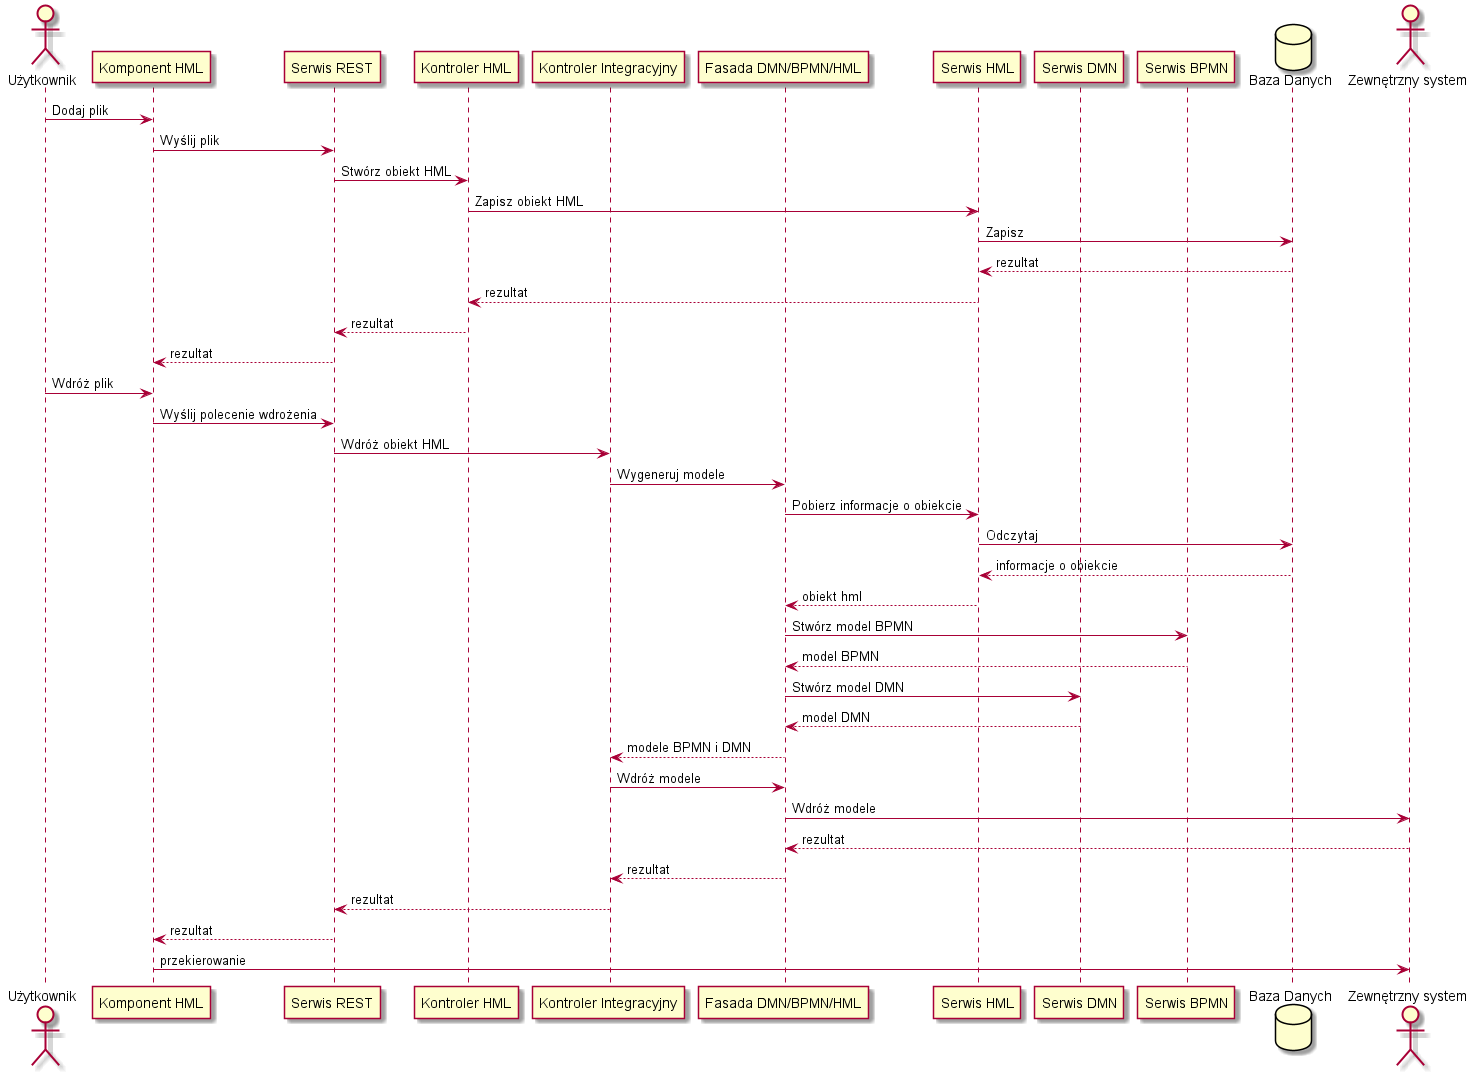
\includegraphics[width=1.4\textwidth, angle=90]{./assets/sequence.png}
    \caption{Schemat interakcji w~aplikacji ,,DAR''}
    \label{fig:sequence}
\end{figure}  
\vspace{1cm}

Jest to koniec rozdziału opisującego projekt aplikacji. W~tym rozdziale została przedstawiona architektura systemu będącego głównym tematem niniejszej pracy. W kolejnym rozdziale zostanie opisana implementacja przedstawionego tutaj projektu, jakie technologie zostały użyte oraz w~jaki sposób zaimplementowane zostały najważniejsze, wspomniane tutaj komponenty aplikacji.




\chapter{Implementacja}
\label{cha:implementacja}
Rozdział opisuje technologie użyte w~pracy oraz przedstawia strukturę bazy danych i~implementacje wydzielonych komponentów. Aplikacja prezentowana jest od strony implementacyjnej. 

%---------------------------------------------------------------------------
\section{Stos technologiczny}
\label{sec:stosTechnologiczny}
Rysunek~\ref{fig:technologyStack} prezentuje technologie użyte podczas implementacji projektu. Stos przedstawiony na rysunku został podzielony na część związaną z~interfejsem użytkownika oraz na część związaną z~serwerem. Dodatkowo pokazana jest technologia, która została wybrana jako zewnętrzny system i~zintegrowana z~aplikacją ,,DAR''. Kolejne podrozdziały pogłębiają temat wybranych technologii.
\begin{figure}
    \centering
    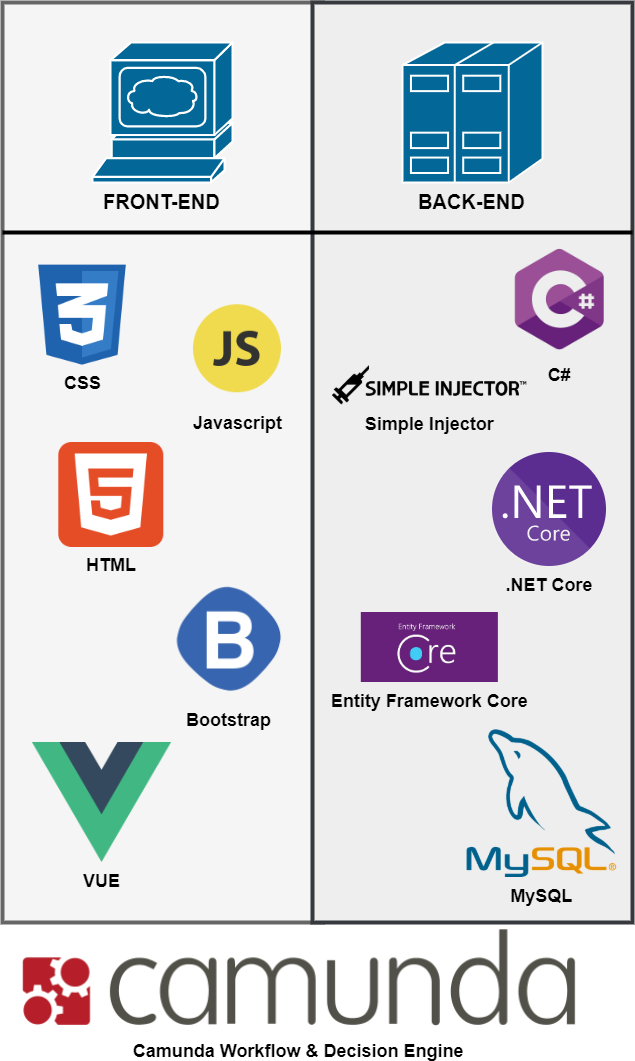
\includegraphics[width=\textwidth, height=0.4\textheight,keepaspectratio]{./assets/technologyStack.png}
    \caption{Stos technologiczny aplikacji ,,DAR''}
    \label{fig:technologyStack}
\end{figure} 

%---------------------------------------------------------------------------
\subsection{Technologie front-end}
\label{sec:frontEndTechnologie}
Przedstawione technologie po stronie lewej rysunku~\ref{fig:technologyStack} są związane z~interfejsem użytkownika. Występuje tutaj podział na języki programowania oraz szkielety aplikacyjne/biblioteki:
\begin{itemize}
    \item \textbf{Języki programowania/Języki komputerowe}
    \begin{itemize}
        \item \textbf{Javascript} -- interpretowany, dynamiczny język programowania wykorzystywany jako główny język skryptowy na stronach internetowych. Według ankiety~\cite{StackSurvey} z~2019 roku, przeprowadzonej na serwisie \emph{StackOverflow}\footnote{Jeden z~najpopularniejszych serwisów dla programistów: \url{https://stackoverflow.com/}.} jest to obecnie najpopularniejszy język świata, bezsprzecznie królujący w~świecie przeglądarek internetowych.
        \item \textbf{HTML} -- \emph{HyperText Markup Language} to język komputerowy stworzony w~celu tworzenia stron internetowych. Umożliwia tworzenie nagłówków, połączeń, ustrukturyzowanych sekcji, paragrafów i wiele innych elementów...
        \item \textbf{CSS} -- \emph{Cascading Style Sheets} to język związany ze stylem dokumentów. Umożliwia on specyfikację, jak pliki są prezentowane użytkownikom -- określa ich styl, ułożenie elementów oraz inne atrybuty. Najczęściej używany razem z~językiem \emph{HTML}. 
    \end{itemize}
    \newpage
    \item \textbf{Szkielety aplikacyjne/Biblioteki}
    \begin{itemize}
        \item \textbf{Bootstrap} -- otwarte oprogramowanie, będące biblioteką \emph{CSS}, nad którą piecze sprawują programiści \emph{Twittera}\footnote{Jeden z~najpopularniejszych portali społecznościowych: \url{https://twitter.com/}.}. Bootstrap usprawnia tworzenie aplikacji internetowych, udostępniając wiele szablonów \emph{HTML} oraz \emph{CSS}, które upiększają stronę.
        \item  \textbf{Vue} -- Szkielet aplikacyjny front-end napisany w~JavaScript, do tworzenia wszelkiego rodzaju interfejsów użytkownika w~tym \emph{Single Page Application}. Usprawnia tworzenie aplikacji internetowych poprzez udostępnienie wielu funkcjonalności, w~tym chociażby manipulowanie drzewem obiektów dokumentu, co pozwala na dynamiczne podmienianie danych na stronie bez konieczności pełnego przeładowania strony. Jest on bardzo podobny do najpopularniejszych szkieletów aplikacyjnych, takich jak \emph{React}\footnote{Więcej na temat \emph{React}: \url{https://pl.reactjs.org/}.} lub \emph{Angular}\footnote{Więcej na temat \emph{Angular}: \url{https://angular.io/}.}. Według wspomnianej już ankiety~\cite{StackSurvey}, \emph{Vue} zyskuje bardzo szybko na popularności.  
    \end{itemize}
\end{itemize}

%---------------------------------------------------------------------------
\subsection{Technologie back-end}
\label{sec:backEndTechnologie}
Przedstawione technologie po stronie prawej rysunku~\ref{fig:technologyStack} są związane z~warstwą logiki oraz danych. Występuje tutaj podział na języki programowania, szkielety aplikacyjne/biblioteki oraz oprogramowania do zarządzania bazą danych:
\newpage
\begin{itemize}
    \item \textbf{Języki programowania}
        \begin{itemize}
            \item \textbf{C\#} -- wysokopoziomowy, obiektowy język programowania. Był on odpowiedzią \emph{Microsoftu}\footnote{Jedna z~największych korporacji świata: \url{https://www.microsoft.com}.} na język \emph{Java}\footnote{Jeden z~najbardziej popularnych, obiektowych języków programowania na świecie: \url{https://www.java.com}.}, ściśle zintegrowany z~platformą \emph{Microsoftu .NET}. Wcześniej używany głównie do tworzenia aplikacji na systemy \emph{Windows}, ale odkąd powstał wieloplatformowy \emph{.NET Core} sytuacja uległa zmianie. Często używany do tworzenia internetowych \emph{API} oraz aplikacji mobilnych dzięki technologi \emph{Xamarin}. Przykładem aplikacji stworzonej przy użyciu C\# jest portal \emph{StackOverflow}.
        \end{itemize}
    \item \textbf{Szkielety aplikacyjne/Biblioteki}
    \begin{itemize}
        \item \textbf{.NET Core} -- a~właściwie \emph{ASP .NET Core}, jest to otwarte oprogramowanie, będące wieloplatformowym szkieletem aplikacyjnym rozwijanym przez \emph{Microsoft} do tworzenia wysoko wydajnych, nowoczesnych, opartych na technologi chmurowej, internetowo połączonych aplikacji. Cały kod tego projektu dostępny jest na platformie \emph{GitHub}\footnote{Zobacz: \url{https://github.com/aspnet/AspNetCore}.}. Dodatkowo dzięki wieloplatformowości umożliwia on tworzenie oraz działanie na platformach, takich jak \emph{Linux} czy \emph{macOS}, a~oprócz tego jest on stworzony z~myślą o konteneryzacji. \emph{ASP .NET Core} wspiera najlepsze metodyki tworzenia aplikacji poprzez promowanie modularności, wbudowane mechanizmy wstrzykiwania zależności czy wsparcie dla rozwiązań chmurowych oraz \emph{gRPC}\footnote{Więcej na temat gRpc: \url{https://grpc.io/}.}. Szkielet aplikacyjny \emph{.NET Core} w~cytowanej już ankiecie~\cite{StackSurvey} portalu \emph{StackOverflow} z~roku 2019, zyskał pierwsze miejsce w~rankingu najlepszych szkieletów aplikacyjnych. Natomiast pod względem wydajności plasuje się w~czołówce (miejsce 10) według rankingu \emph{TechEmpower}~\cite{WebBenchmark}, wyprzedzając takie szkielety aplikacyjne jak \emph{Django} (miejsce 213), \emph{Spring} (miejsce 245), czy \emph{Ruby on Rails} (miejsce 215).
        \item \textbf{Entity Framework Core} -- jest to ORM (\emph{Object-Relational Mapper}), czyli narzędzie pozwalające programistom działać z~danymi w~stylu obiektowym. Jego głównym zadaniem jest mapowanie obiektów zdefiniowanych w~aplikacji w~wybranym języku programowania, do danych przechowywanych w~relacyjnej bazie danych. Narzędzie to bardzo ułatwia pracę z~bazą danych, ukrywając za abstrakcjami połączenia z~bazą danych, wszelkie konwersje do języka \emph{SQL} oraz tworzenie struktur bazy danych.
        \item \textbf{Simple Injector} -- biblioteka służąca jako kontener wstrzykiwania zależności. Szkielet aplikacyjny \emph{.NET Core} posiada wbudowane narzędzie do wstrzykiwania zależności jednak \emph{Simple Injector} działa opierając się na nim i~rozbudowując jego możliwości. Jego głównym zadaniem jest pilnowanie oraz zarządzanie cyklem życia obiektów w~aplikacji, poprzez zastosowanie odwrócenia sterowania~\cite{DI}.
    \end{itemize}
    \newpage
    \item \textbf{Oprogramowanie do zarządzania bazą danych}
        \begin{itemize}
            \item \textbf{MySQL} -- jest to otwarte oprogramowanie, będące systemem do zarządzania relacyjnymi bazami danych, opierającym się na modelu klient-serwer. Odpowiada on za stworzenie bazy danych i~odpowiednie przechowywanie oraz zarządzanie informacjami. Komunikacja opiera się na języku SQL (\emph{Structured Query Language}), służącym do manipulowania danymi.
        \end{itemize}
\end{itemize}

%---------------------------------------------------------------------------
\subsection{Zewnętrzny System}
\label{sec:zewnętrznySystem}
\emph{Camunda} została wybrana jako zewnętrzny system do zarządzania modelami procesów oraz decyzji. Jest to otwarte oprogramowanie napisane w języku \emph{Java}, pozwalające na uruchomienie wykonywalnych modeli procesów, ewaluację decyzji oraz monitorowanie całego przepływu działań procesu. Najważniejsze komponenty, które udostępnia \emph{Camunda} w~kontekście niniejszej pracy to:
\begin{itemize}
    \item \textbf{Silnik}
        \begin{itemize}
            \item \textbf{Process Engine} -- silnik napisany w~języku \emph{Java}, umożliwiający uruchamianie procesów w~notacji \emph{BPMN} oraz decyzji w~notacji \emph{DMN}.
        \end{itemize}
    \item \textbf{Aplikacje internetowe}
        \begin{itemize}
            \item \textbf{REST API} -- \emph{API} umożliwiające dostęp do wspomnianego wcześniej silnika oraz platformy zarządzającej procesami i~decyzjami. Głównie wykorzystywane w~celu wdrożenia modelów \emph{BPMN} oraz \emph{DMN} do platformy.
            \item \textbf{Camunda Tasklist} -- część platformy do zarządzania procesami i~decyzjami. Umożliwia uruchomienie procesu oraz wykonywanie zadań użytkownika, np. podanie odpowiednich danych, potrzebnych do działania procesu.
            \item \textbf{Camunda Cockpit} -- część platformy do zarządzania procesami i~decyzjami. Umożliwia obserwację i~edycję modeli \emph{BPMN} oraz \emph{DMN}, oraz monitorowanie wykonywanych procesów i~ewaluowanych decyzji.
        \end{itemize}
\end{itemize}

Pomimo że \emph{Camunda} jest w~wersji podstawowej otwartym oprogramowaniem, w~kontekście niniejszej pracy wymagana jest edycja typu \emph{Enterprise} będąca wersją płatną. Wynika to z~faktu, że modele \emph{DMN} tworzone przez aplikację \emph{DAR} nie są wypełnione regułami -- ze względu na brak takowych w~diagramach \emph{ARD}. W utworzonych tabelach decyzyjnych należy uzupełnić reguły, tak aby decyzje mogły być ewaluowane. Ta możliwość jest udostępniona tylko w~wersji płatnej.

%---------------------------------------------------------------------------
\section{Schemat bazy danych}
\label{sec:schematBazyDanych}
Dzięki wspomnianemu wcześniej \emph{Entity Framework Core}, wszystkie klasy, które zostały zmapowane ze schematu pliku \emph{HML} do kodu w~języku \emph{C\#}, automatycznie zostały użyte do budowy tabel w~relacyjnej bazie danych. Rysunek~\ref{fig:databaseScheme} przedstawia efekt tego zabiegu. 
\begin{figure}
    \centering
    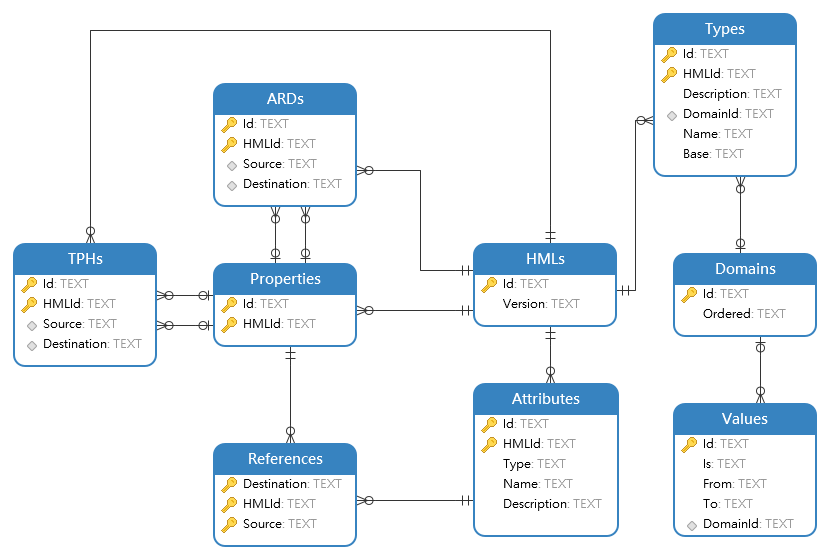
\includegraphics[width=\textwidth,height=0.4\textheight,keepaspectratio]{./assets/databaseScheme.png}
    \caption{Schemat bazy danych aplikacji ,,DAR''}
    \label{fig:databaseScheme}
\end{figure}

Warto przyjrzeć się bliżej poszczególnym tabelom:
\begin{itemize}
    \item \textbf{Tabela HMLs} -- serce całego schematu. Posiada jeden klucz główny \emph{Id}, identyfikujący poszczególne pliki \emph{HML}. Dodatkowo określa wersję danego pliku.
    \item \textbf{Tabela Properties} -- reprezentuje właściwości opisane w~plikach. Posiada dwa klucze, jeden główny, będący złożeniem \emph{Id} oraz \emph{HMLId}, służący do identyfikacji, oraz drugi obcy \emph{HMLId}, będący połączeniem do tabeli \emph{HMLs}.
    \item \textbf{Tabela Attributes} -- reprezentuje atrybuty opisane w~plikach. Posiada dwa klucze, jeden główny, będący złożeniem \emph{Id} oraz \emph{HMLId}, służący do identyfikacji, oraz drugi obcy \emph{HMLId}, będący połączeniem do tabeli \emph{HMLs}. Zawiera dodatkowo informacje o atrybutach, takie jakie nazwa, opis oraz typ danych.
    \item \textbf{Tabela References} -- pośredniczy pomiędzy właściwościami, a~atrybutami. Posiada trzy klucze. Jeden podstawowy będący złożeniem \emph{Destination}, \emph{Source} oraz \emph{HMLId}, służący do identyfikacji oraz dwa obce: złożenie \emph{Source} oraz \emph{HMLId}, będące połączeniem do tabeli \emph{Properties} i~złożenie \emph{Destination} oraz \emph{HMLId}, będące połączeniem do tabeli \emph{Attributes}.
    \item \textbf{Tabela Types} -- reprezentuje typy danych opisane w~plikach. Posiada trzy klucze. Jeden podstawowy \emph{Id}, służący do identyfikacji oraz dwa obce: \emph{HMLId} będący połączeniem do tabeli \emph{HMLs} oraz \emph{DomainId}, będący połączeniem do tabeli \emph{Domains}. Dodatkowo określa takie właściwości, jak opis typu, nazwa oraz podstawa (przykładowo numeryczna).
    \item \textbf{Tabela Values} -- reprezentuje możliwe wartości danego typu. Posiada dwa klucze. Jeden podstawowy \emph{Id}, służący do identyfikacji oraz jeden obcy \emph{DomainId}, będący połączenim do tabeli \emph{Domains}. Dodatkowo określa różne możliwości związane z~wartościami, typu przedziały wartości, czy jest to wartość numeryczna lub konkretna wartość.
    \item \textbf{Tabela Domains} -- reprezentuje dziedziny opisane w~pliku i~pośredniczy między tabelami \emph{Types} and \emph{Values}. Posiada jeden klucz główny \emph{Id}, służący do identyfikacji.
    \item \textbf{Tabela ARDs} -- reprezentuje zależności między właściwościami. Posiada cztery klucze: jeden podstawowy złożony z~\emph{Id} oraz \emph{HMLId}, służący do identyfikacji i trzy obce: \emph{HMLId}, będące połączeniem do tabeli \emph{HMLs} oraz dwa złożenia: \emph{HMLId} i~\emph{Source}, będące połączeniem do tabeli \emph{Properties}, do właściwości niezależnej oraz złożenie \emph{HMLId} i~\emph{Destination}, będące połączeniem do tabeli \emph{Properties}, do właściwości zależnej.
    \item \textbf{Tabela TPHs} -- właściwie niewykorzystywana, reprezentuje historię zależności między właściwościami. Posiada cztery klucze: jeden podstawowy złożony z~\emph{Id} oraz \emph{HMLId}, służący do identyfikacji oraz trzy obce: złożenie \newline \emph{HMLId} i~\emph{Source}, będące połączeniem do tabeli \emph{Properties}, do właściwości niezależnej, złożenie \emph{HMLId} i~\emph{Destination}, będące połączeniem do tabeli \emph{Properties}, do właściwości zależnej oraz \emph{HMLId}, będące połączeniem do tabeli \emph{HMLs}.
\end{itemize} 

%---------------------------------------------------------------------------
\section{Schemat klas}
\label{sec:schematKlas}
Rysunek~\ref{fig:classDiagram1} przedstawia najistotniejsze klasy aplikacji. Pominięte zostały klasy związane z~infrastrukturą, określające jak szkielet aplikacyjny \emph{ASP .NET Core} ma obsługiwać przychodzące zapytania \emph{HTTP}, którego serwera lub której bazy danych ma używać. Dodatkowo niezaprezentowane zostały encje, będące prostymi klasami bez żadnej logiki, zawierającymi jedynie pola, gdyż zostały wygenerowane one automatycznie na podstawie specyfikacji plików \emph{ARD}, \emph{BPMN} oraz \emph{DMN}.
\begin{figure}
    \centering
    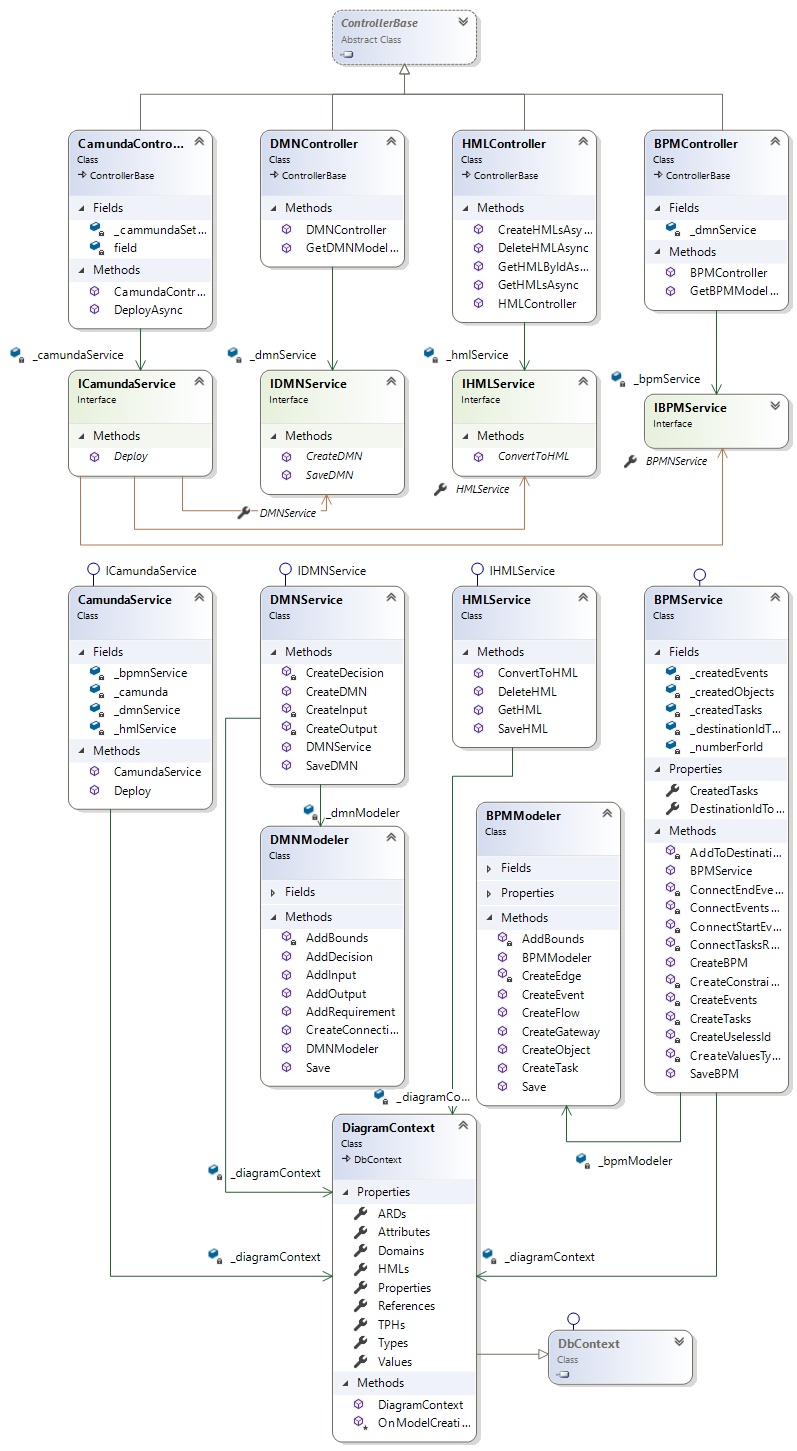
\includegraphics[width=\textwidth, height=0.95\textheight,keepaspectratio]{./assets/classDiagram.png}
    \caption{Schemat klas wchodzących w~skład \emph{REST API} aplikacji ,,DAR''}
    \label{fig:classDiagram1}
\end{figure}

Na rysunku~\ref{fig:classDiagram1} widać, że wszystkie komponenty typu \emph{Kontroler}, dziedziczą po bazowej klasie \emph{ControllerBase}, należącej do \emph{ASP .NET Core}. Dzięki temu, aplikacja może w~łatwy sposób nawigować adresy w~stylu \emph{REST} do konkretnej klasy i~metody. Kontrolery przyjmują zapytania \emph{HTTP} oraz związane z~nimi dane, walidują je, a~następnie przekazują do komponentów implementujących logikę biznesową, w~tym przypadku serwisów. Serwisy występujące w~kontrolerach, opierają się na interfejsach -- jest to związane z~wspomnianym już wstrzykiwaniem zależności i~odwróceniem sterowania. \emph{ASP .NET Core} promuje programowanie do interfejsów. Na diagramie~\ref{fig:classDiagram1} widać, że każdy interfejs został zaimplementowany i~to właśnie te implementacje są wstrzykiwane w~czasie działania aplikacji do kontrolerów. Dodatkowo serwisy \emph{BPM}, \emph{DMN} oraz \emph{HML} posiadają referencje do klasy \emph{DiagramContext}, dziedziczącej po klasie \emph{DbContext} -- klasie należącej do opisywanego już \emph{Entity Framework Core}. Umożliwia ona komunikację z~bazą danych. Wszystkie pola występujące w~klasie \emph{DiagramContext} są odwzorowane w~bazie danych jako tabele (rysunek~\ref{fig:databaseScheme}) -- serwisy korzystają z~tej klasy, jak z~repozytorium, używając wspomnianych pól aby, pobierać/edytować/usuwać/dodawać dane. Serwisy \emph{BPMN} oraz \emph{DMN} zawierają również referencję do odpowiednich klas z~zakończeniem ,,Modeler''. Są to klasy pomocnicze pozwalające na dodawanie diagramowych obiektów związanych z~modelami \emph{BPMN} oraz \emph{DMN} do plików tych modeli -- takie obiekty muszą posiadać wymiary oraz współrzędne.
\vspace{1cm}

Jest to koniec rozdziału opisującego implementacje aplikacji. W~tym rozdziale przedstawione zostały technologie użyte w~celu stworzenia systemu, a~także schematy implementacji najważniejszych elementów aplikacji. W kolejnym rozdziale wykorzystane zostaną opisane tutaj elementy i~przedstawione zostanie działanie zaimplementowanej aplikacji na konkretnym przykładzie.





\chapter{Ewaluacja}
\label{cha:ewaluacja}
Rozdział prezentuje działanie aplikacji na przykładzie procesu obliczania kwoty ubezpieczenia samochodowego. Przedstawione zostały wybrane najważniejsze funkcjonalności systemu.

%---------------------------------------------------------------------------
\section{Model ARD}
\label{sec:modelARD}
Przykład, na którym zostanie zaprezentowana aplikacja, obrazuje proces związany z~obliczaniem kwoty płatności na rzecz ubezpieczenia samochodowego. Jak wiadomo kwota takiego ubezpieczenia zależy od wielu zmiennych, takich jak liczba wypadków, wiek kierowcy czy rodzaj samochodu. Rysunek~\ref{fig:ardInsuranceExample} prezentuje diagram \emph{ARD}, który mógłby zostać stworzony przez analityka biznesowego, jako prototyp takiego procesu.
\begin{figure}
    \centering
    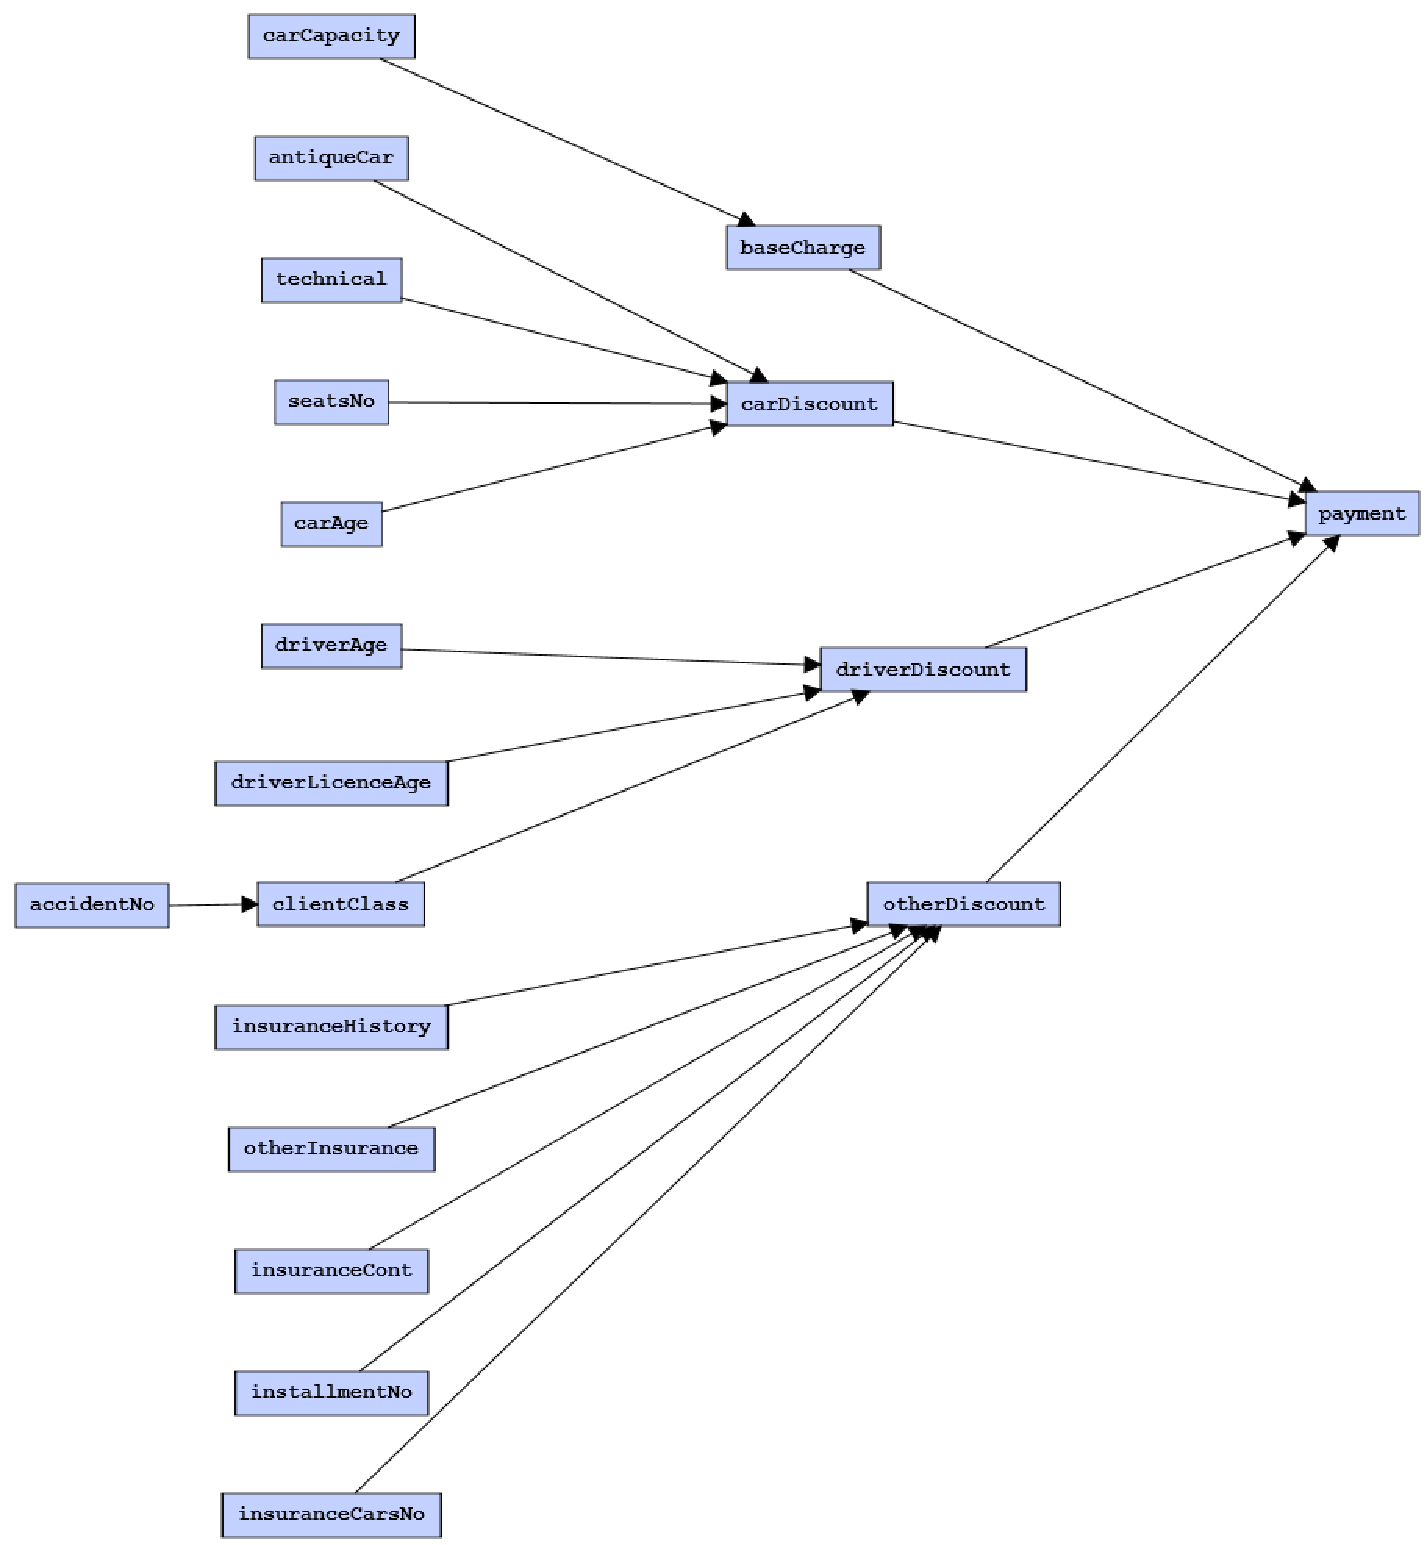
\includegraphics[width=\textwidth]{./assets/ardInsuranceExample.pdf}
    \caption{Diagram \emph{ARD} będący prototypem procesu obliczania kwoty ubezpieczenia samochodowego. Przykład opracowany na bazie studium przypadku przygotowanego w~ramach ewaluacji metodyki Semantycznia Inżynieria Wiedzy~\cite{gjn2011hab}}
    \label{fig:ardInsuranceExample}
\end{figure} 
Tabela~\ref{tab:att} opisuje wszystkie własności, przedstawione na diagramie \emph{ARD} (rysunek~\ref{fig:ardInsuranceExample}). Podany jest ich typ, zakres oraz krótki opis.
\begin{table}
    \begin{tabular}{|p{3.6cm}|p{1.4cm}|p{1.8cm}|p{7cm}|}
    %\cline{1-5}
    \hline
    \textbf{~nazwa~} & \textbf{~typ~} & \textbf{~zakres~} & \textbf{~opis~}\\ \hline\hline
    \texttt{accidentNo} & integer & [0;inf] & liczba kolizji spowodowanych w~okresie ostatnich 12 miesięcy\\ \hline
    \texttt{clientClass} & integer & [-1;9] & klasa jaką posiada klient\\ \hline
    \texttt{carCapacity} & integer & [0;inf] & pojemność silnika [$cm^{3}$]\\ \hline
    \texttt{baseCharge} & integer & [0;inf] & stawka podstawowa w~[$PLN$]\\ \hline
    \texttt{driverAge} & integer & [16;inf] & wiek właściciela pojazdu\\ \hline
    \texttt{driverLicenseAge} & integer & [0;inf] & okres posiadania prawa jazdy przez właściciela pojazdu \\ \hline
    \texttt{driverDiscount} & integer & --- & suma zniżek \texttt{driverAge} i~\texttt{drLicAge} \\ \hline
    \texttt{carAge} & integer & [0;inf] & wiek samochodu\\ \hline
    \texttt{antiqueCar} & boolean & [true; false] & pojazd historyczny \\ \hline
    \texttt{seatsNo} & integer & [2;9] & liczba siedzeń w~pojeździe \\ \hline
    \texttt{technical} & boolean & [true; false] & aktualne badania techniczne\\ \hline
    \texttt{carDiscount} & integer & --- & suma zniżek za \texttt{carAge}, \texttt{historiCar}, \newline \texttt{noSeats} i~\texttt{technical}\\ \hline
    \texttt{installmentNo} & integer & [1;2] & liczba rat \\ \hline
    \texttt{insuranceCont} & boolean & [true; false] & kontynuacja ubezpieczenia \\ \hline
    \texttt{insuranceCarsNo} & integer & [0;inf] & liczba ubezpieczonych samochodów\\ \hline
    \texttt{otherInsurance} & boolean & [true; false] & inne ubezpieczenia\\ \hline
    \texttt{insuranceHistory} & integer & [0;inf] & historia ubezpieczenia \\ \hline
    \texttt{otherDiscount} & integer & --- & suma zniżek za \texttt{noRates}, \texttt{contIns}, \newline \texttt{noCarsIns}, \texttt{otherIns}, \texttt{insHistory} \\ \hline
    \texttt{payment} & float & [0;inf] & ostateczna opłata za ubezpiecznie danego pojazdu w~[$PLN$]\\ \hline
    \end{tabular}\vspace{-2mm}
       \caption{Opis własności w~prototypie procesu obliczania kwoty ubezpieczenia samochodowego. Przykład opracowany na bazie studium przypadku przygotowanego w~ramach ewaluacji metodyki Semantycznia Inżynieria Wiedzy~\cite{gjn2011hab} }
       \label{tab:att}
    \vspace{-3mm}
\end{table} 
Na tej podstawie stworzony został plik \emph{HML}. Zawartość pliku, ze względu na spory rozmiar, nie jest tutaj wylistowana.


%---------------------------------------------------------------------------
\section{Interfejs użytkownika}
\label{sec:interfejsUżytkownika}
Po uruchomieniu aplikacji pierwszym widokiem, z~którym ma do czynienia użytkownik jest domyślny ekran z~omawianego w~rozdziale~\ref{cha:projektAplikacji} komponentu \emph{Home}, co prezentuje rysunek~\ref{fig:darHome}.
\begin{figure}
    \centering
    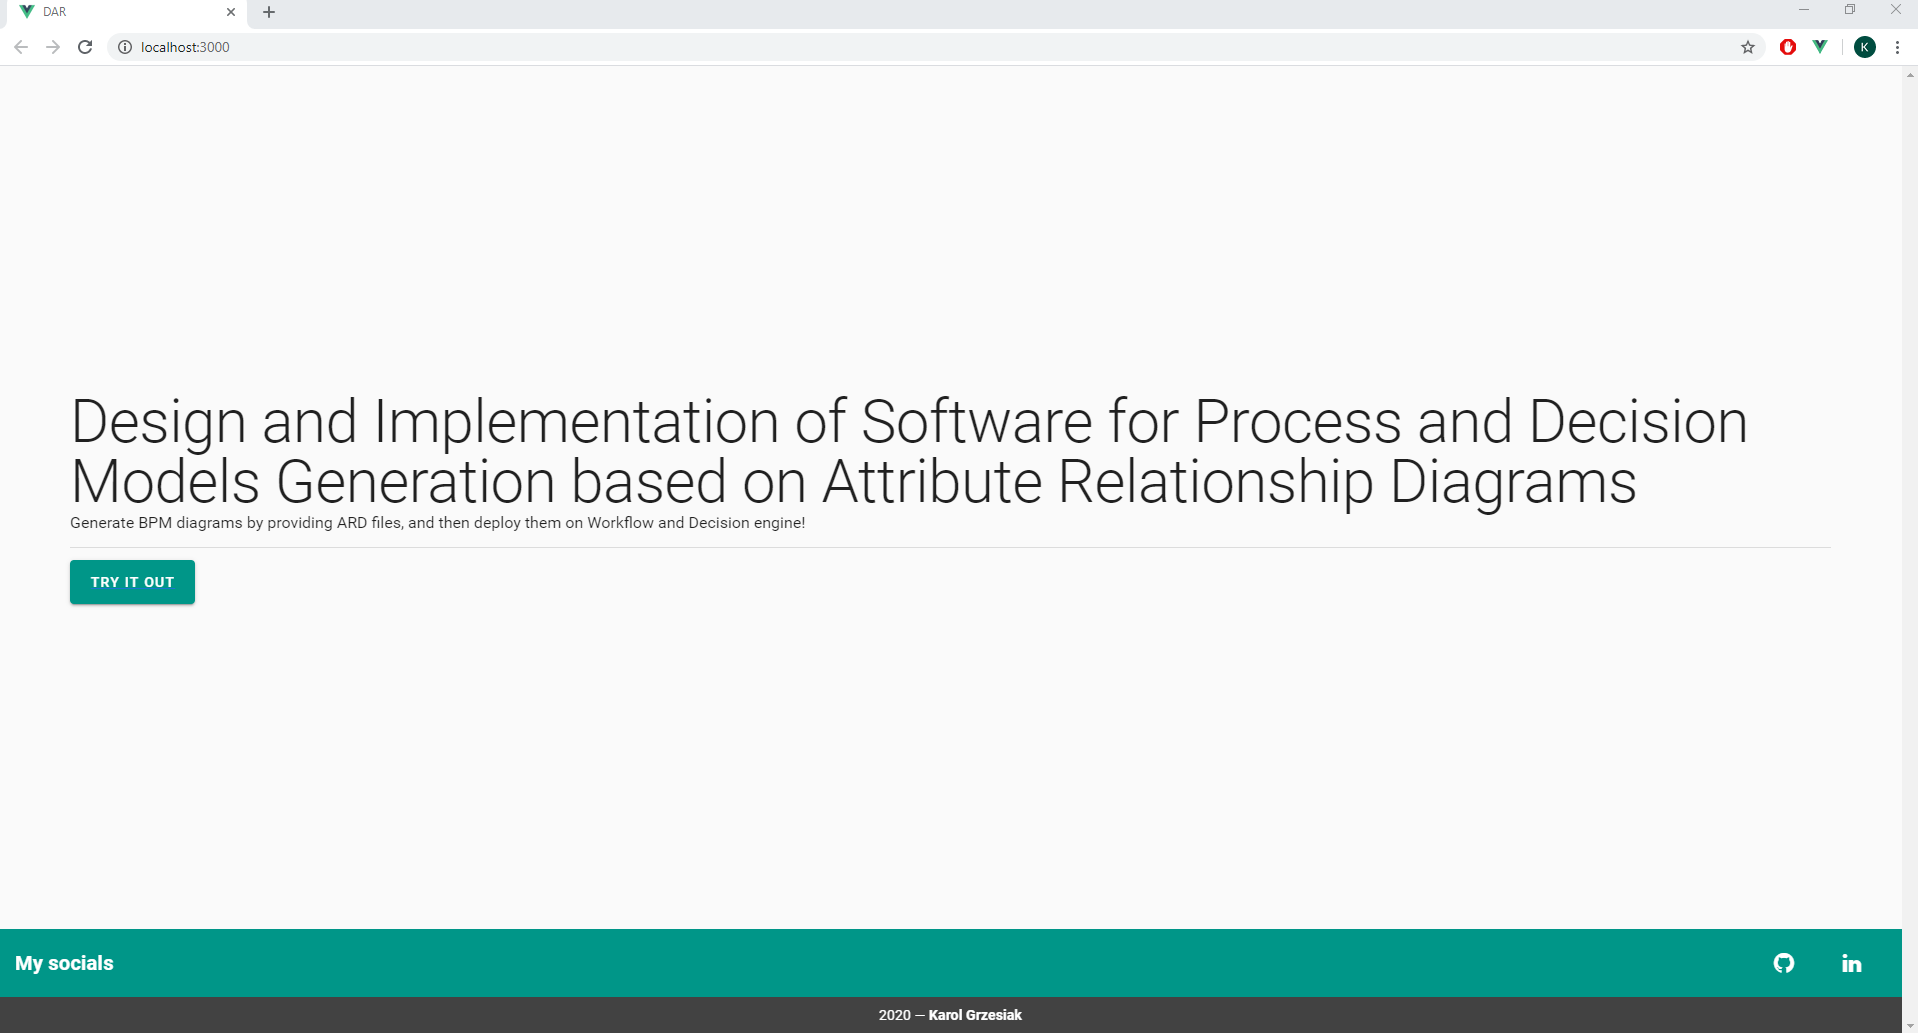
\includegraphics[width=\textwidth]{./assets/darHome.png}
    \caption{Domyślny ekran aplikacji ,,DAR''}
    \label{fig:darHome}
\end{figure} 

Po naciśnięciu przycisku ,,TRY IT OUT'', użytkownik zostaje przeniesiony do głównej części interfejsu użytkownika, czyli do widoku z~komponentu \emph{HML}. W tym miejscu prezentowane są wszystkie pliki \emph{HML}, z~których informacje znajdują się w~bazie danych. Użytkownik ma możliwość dodania nowego pliku, a~także wykonania akcji na plikach już dodanych. W przypadku naciśnięcia na któryś z~wyświetlanych plików, aplikacja prezentuje dwa przyciski: ,,DEPLOY'' oraz ,,DELETE''. Naciśnięcie pierwszego przycisku powoduje generację modeli \emph{BPMN} oraz \emph{DMN}, a~następnie wdrożenie ich na platformę \emph{Camunda}, aby finalnie przenieść użytkownika na wspomnianą platformę. Naciśnięcie drugiego przycisku powoduje usunięcie pliku z~bazy danych. Rysunek~\ref{fig:darHML} przedstawia opisany interfejs po wgraniu dwóch plików \emph{HML}. Plik ,,example'' to plik zawierający wcześniej opisywany model \emph{ARD}. Dalsza część rozdziału opisuję scenariusz, w~którym naciśnięty zostaje zielony przycisk pod plikiem ,,example'' i~plik zostaje wdrożony.  
\begin{figure}
    \centering
    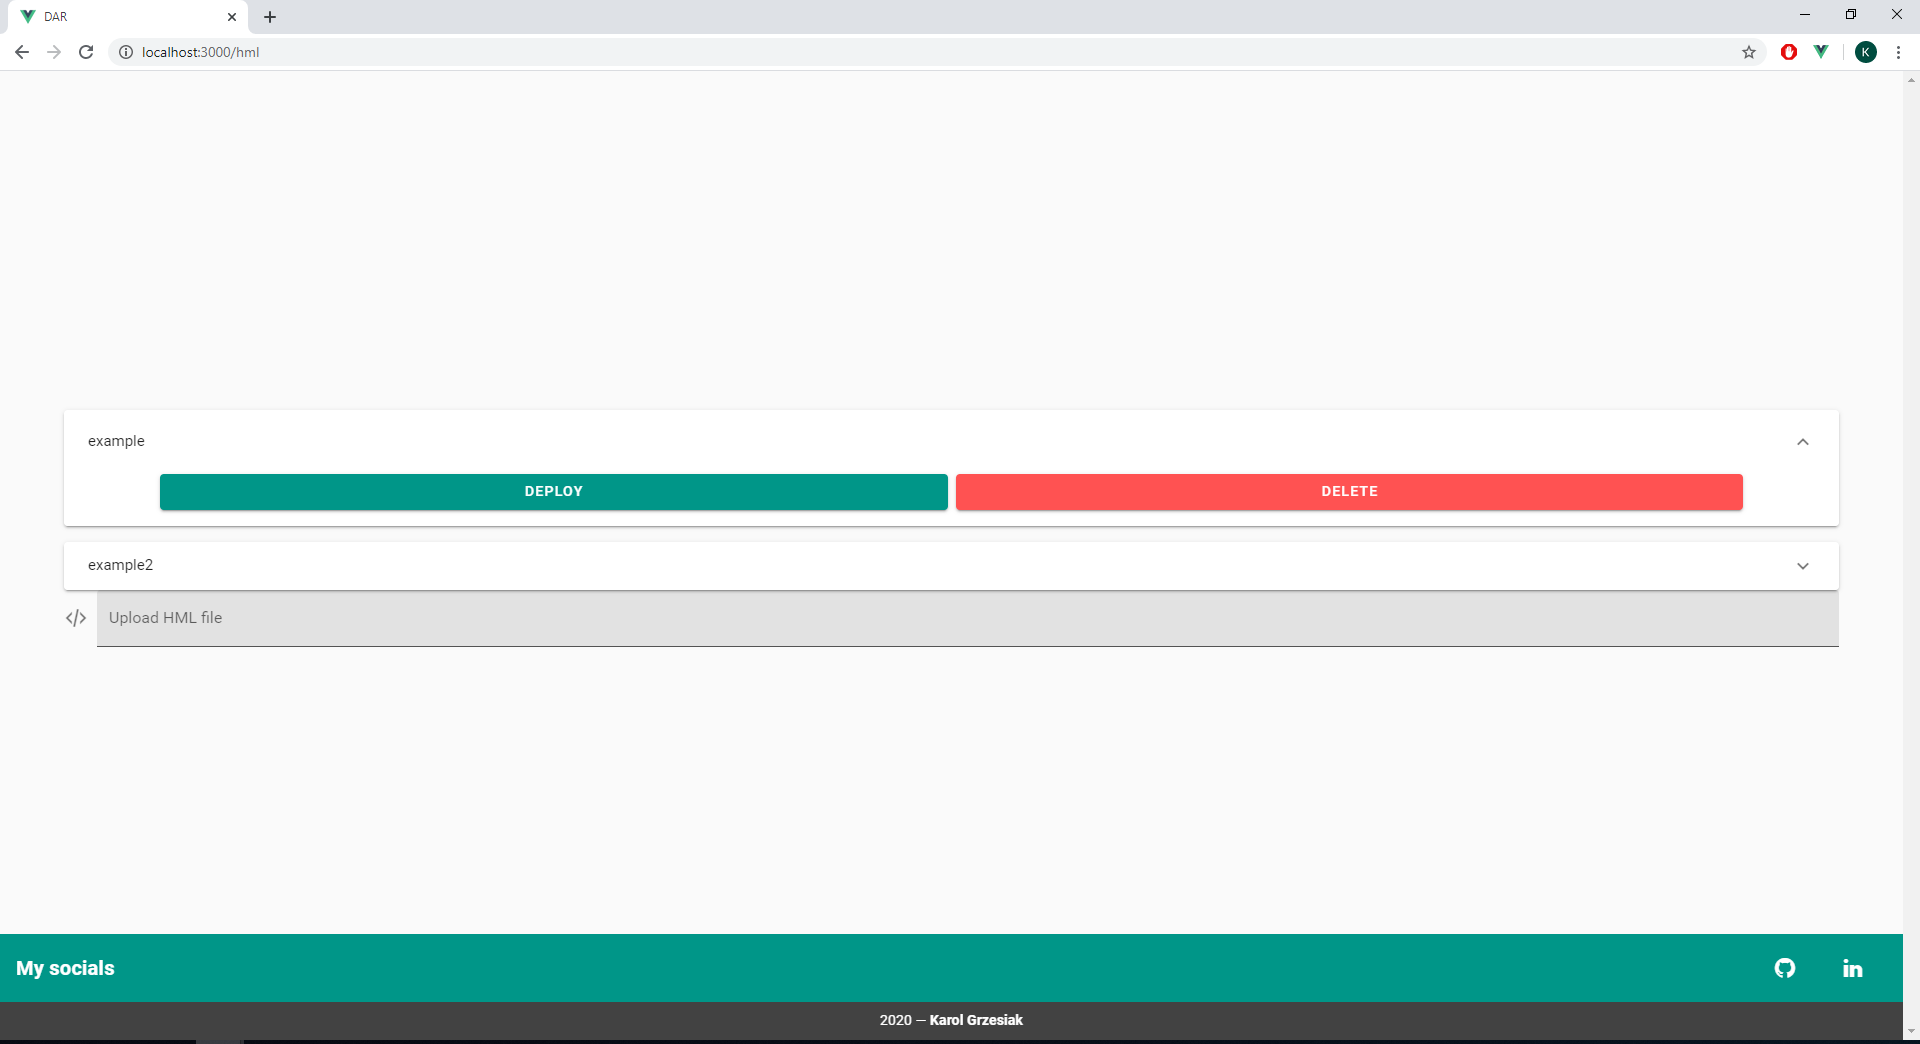
\includegraphics[width=\textwidth]{./assets/darHML.png}
    \caption{Główny ekran interfejsu użytkownika aplikacji ,,DAR''}
    \label{fig:darHML}
\end{figure}

%---------------------------------------------------------------------------
\section{Camunda}
\label{sec:camunda}
Po wdrożeniu pliku zawierającego model opisany w~podrozdziale~\ref{sec:modelARD} użytkownik zostaje przeniesiony na platformę \emph{Camunda}. Domyślny widok, który zostaje mu zaprezentowany przedstawia rysunek~\ref{fig:camundaDefault}. Do dyspozycji są trzy aplikacje, najważniejsze z nich to \emph{Camunda Cockpit} oraz \emph{Camunda Tasklist}. Były one opisywane w~rozdziale~\ref{sec:zewnętrznySystem}.
\begin{figure}
    \centering
    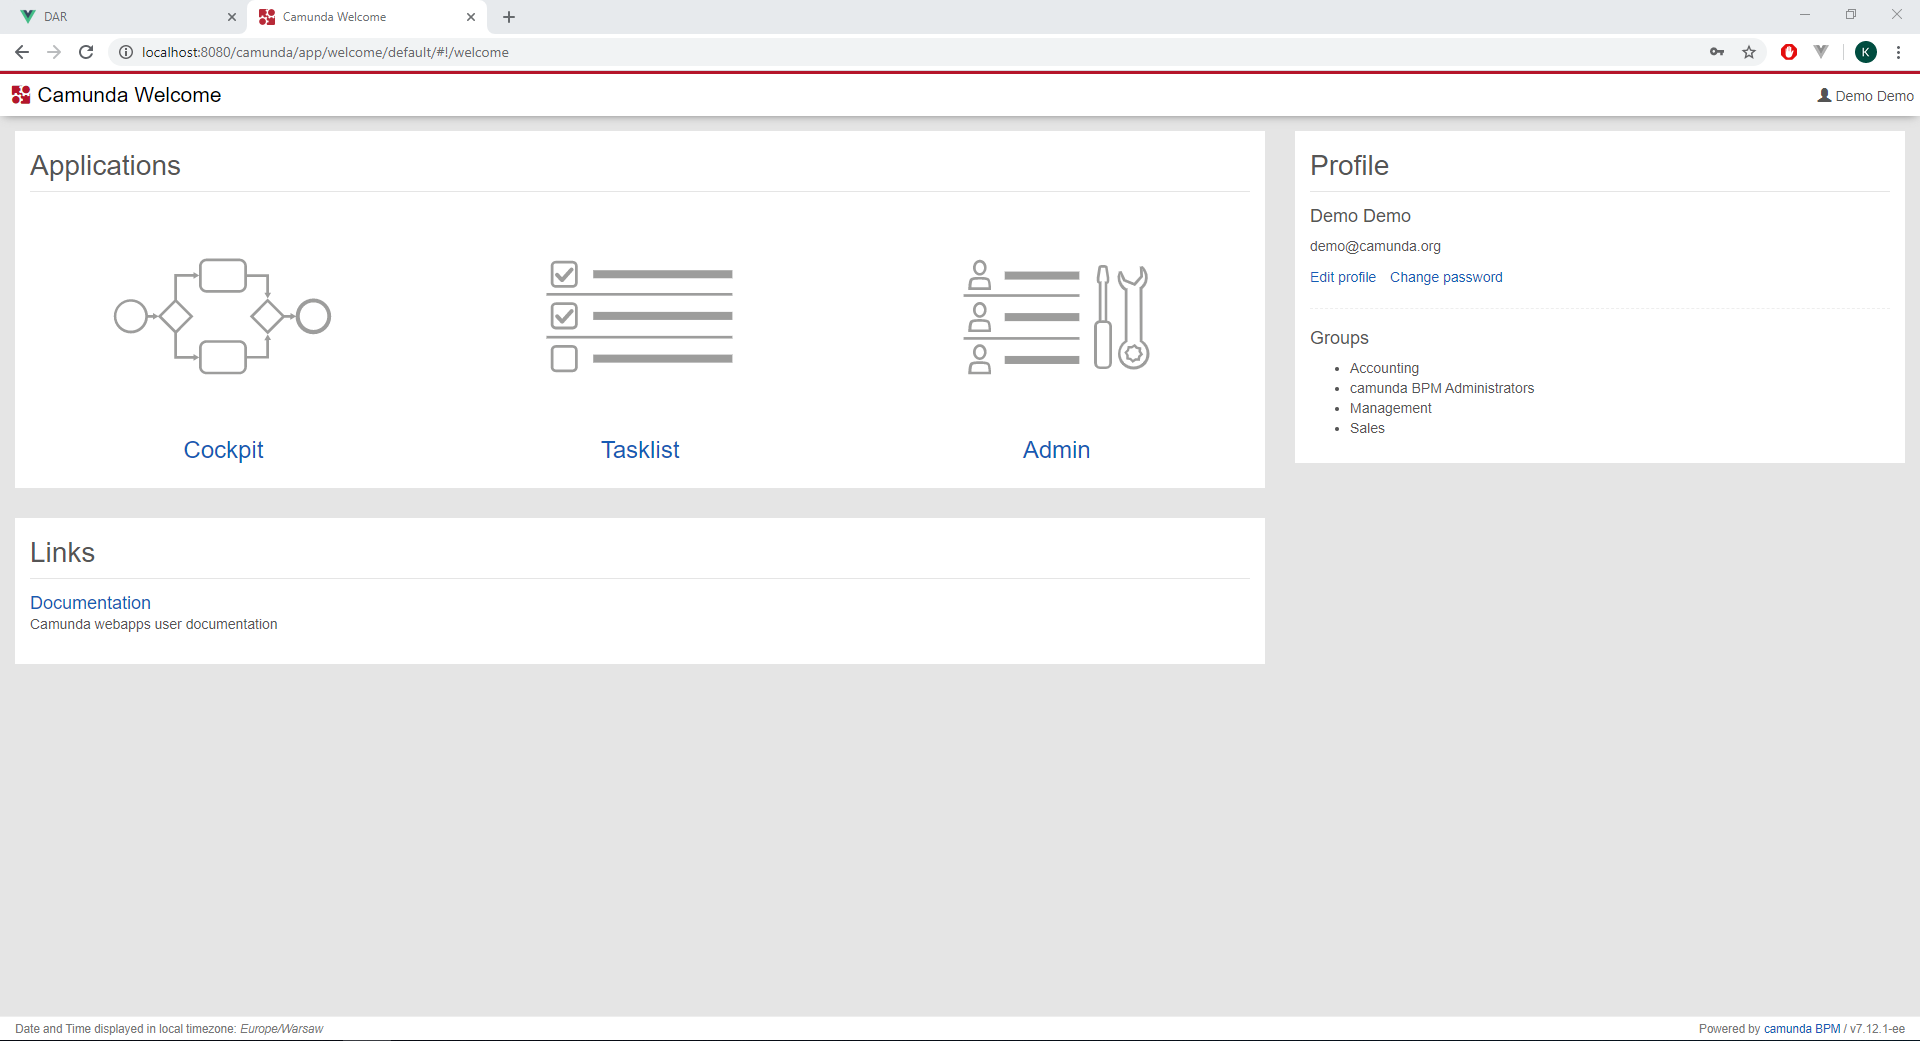
\includegraphics[width=\textwidth]{./assets/camundaDefault.png}
    \caption{Domyślny ekran platformy \emph{Camunda} po wdrożeniu pliku \emph{HML}}
    \label{fig:camundaDefault}
\end{figure}

Rysunek~\ref{fig:camundaCockpitDefault} przedstawia domyślny ekran aplikacji \emph{Camunda Cockpit}. Znajduje się na nim wiele metryk służących do analizy działań na platformie oraz informację o uruchomionych procesach.
\begin{figure}
    \centering
    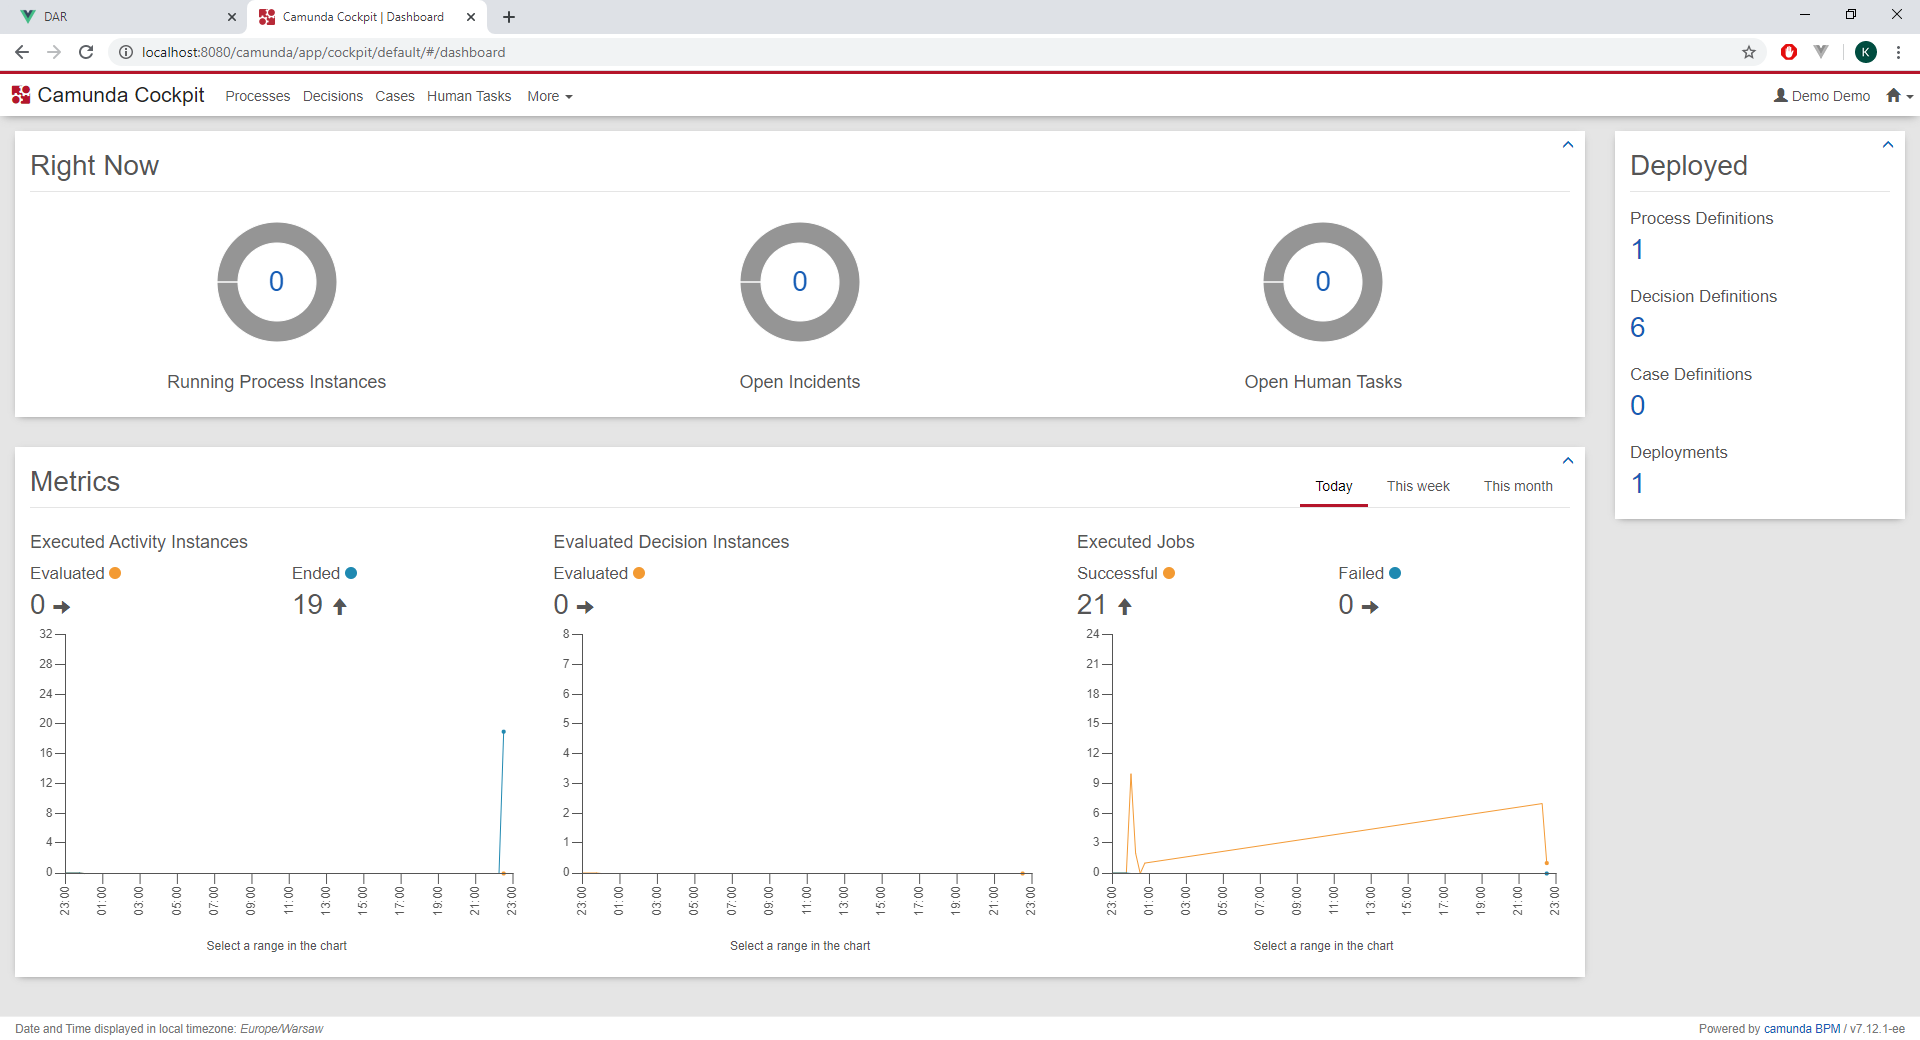
\includegraphics[width=\textwidth]{./assets/camundaCockpitDefault.png}
    \caption{Domyślny ekran \emph{Camunda Cockpit}}
    \label{fig:camundaCockpitDefault}
\end{figure}
Przechodząc do zakładki ,,Deployments'' (,,More`` $\rightarrow$ ,,Deployments``) prezentowane są wszystkie wdrożenia, które miały miejsce. Jak widać na rysunku~\ref{fig:camundaCockpitDeployments} pojawiło się tutaj wdrożenie pliku ,,example'', a~wraz z~nim wygenerowane modele w~notacjach \emph{BPMN} oraz \emph{DMN}. Rysunki~\ref{fig:camundaExampleBPMN} oraz~\ref{fig:camundaExampleDMN} prezentują stworzone wspomniane modele.
\begin{figure}
    \centering
    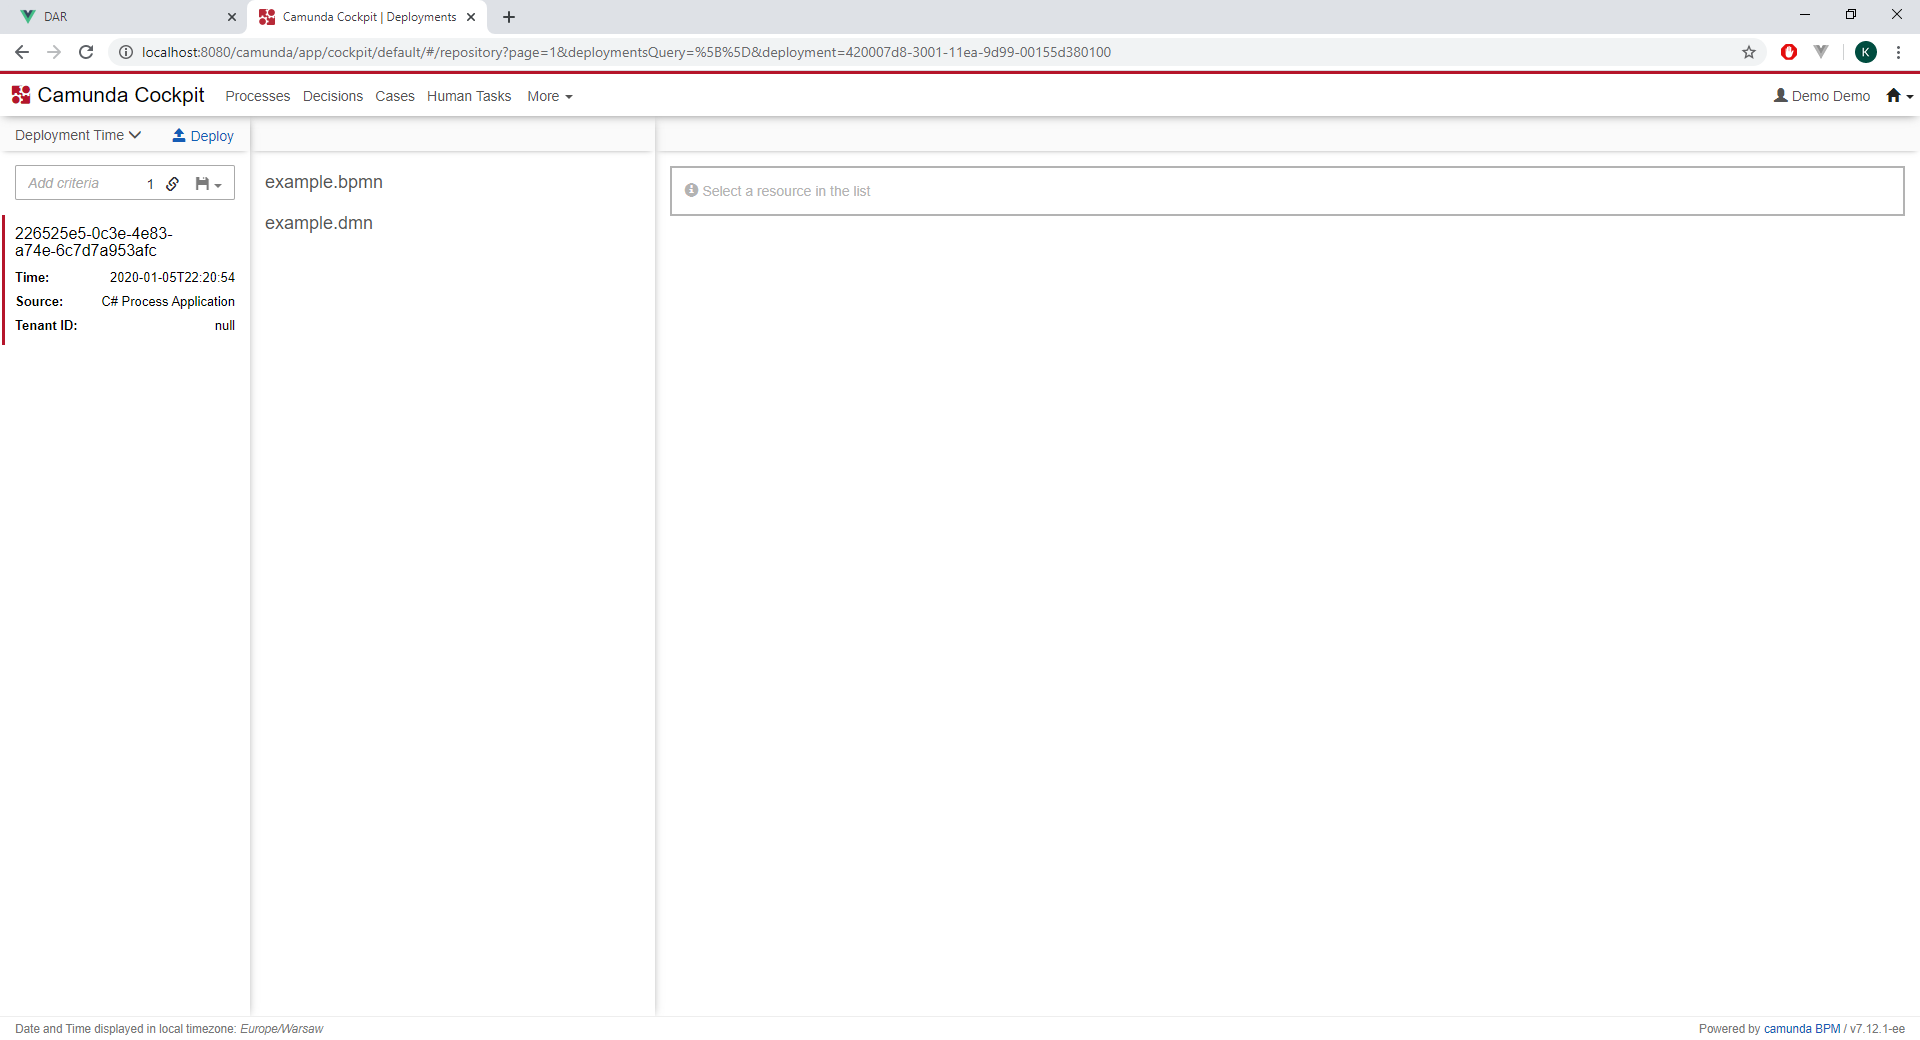
\includegraphics[width=\textwidth]{./assets/camundaCockpitDeployments.png}
    \caption{Ekran wdrożeń \emph{Camunda Cockpit}}
    \label{fig:camundaCockpitDeployments}
\end{figure}
\begin{figure}
    \centering
    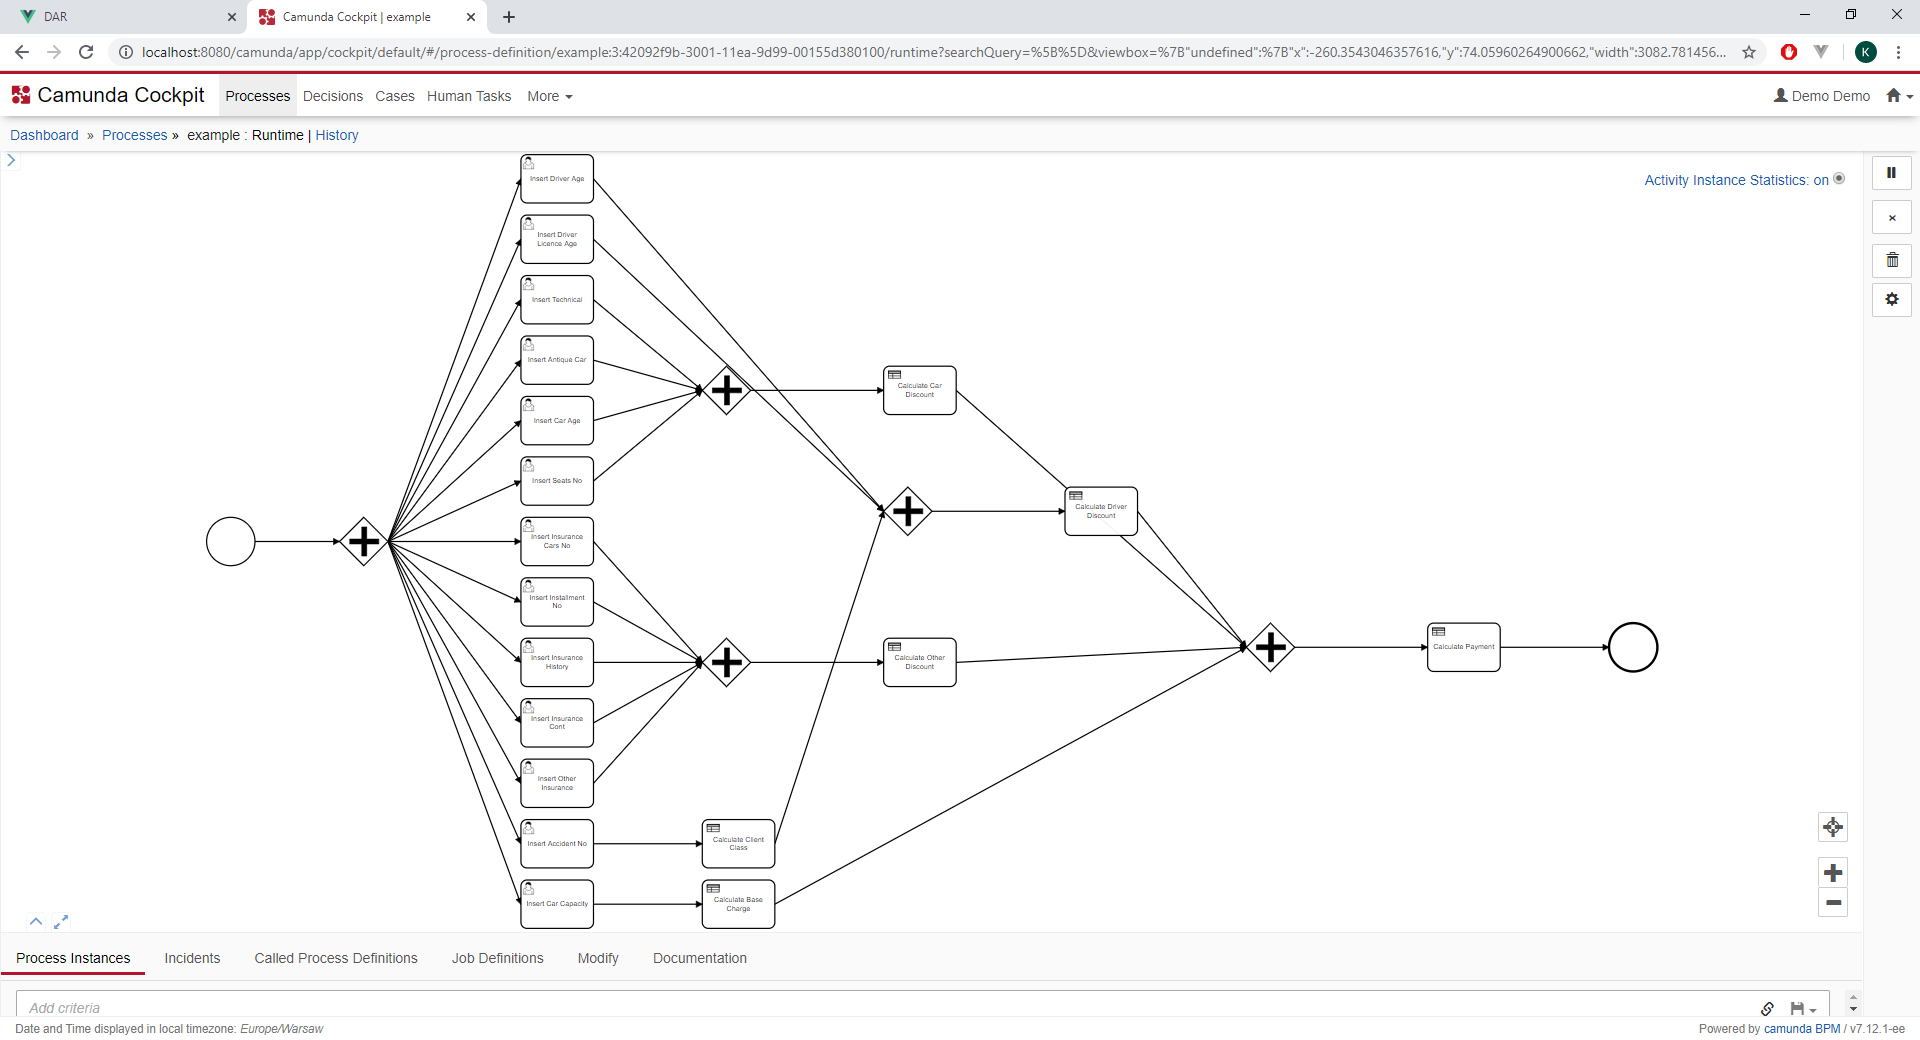
\includegraphics[width=\textwidth]{./assets/camundaExampleBPMN.png}
    \caption{Model \emph{BPMN} pliku ,,example''}
    \label{fig:camundaExampleBPMN}
\end{figure}
\begin{figure}
    \centering
    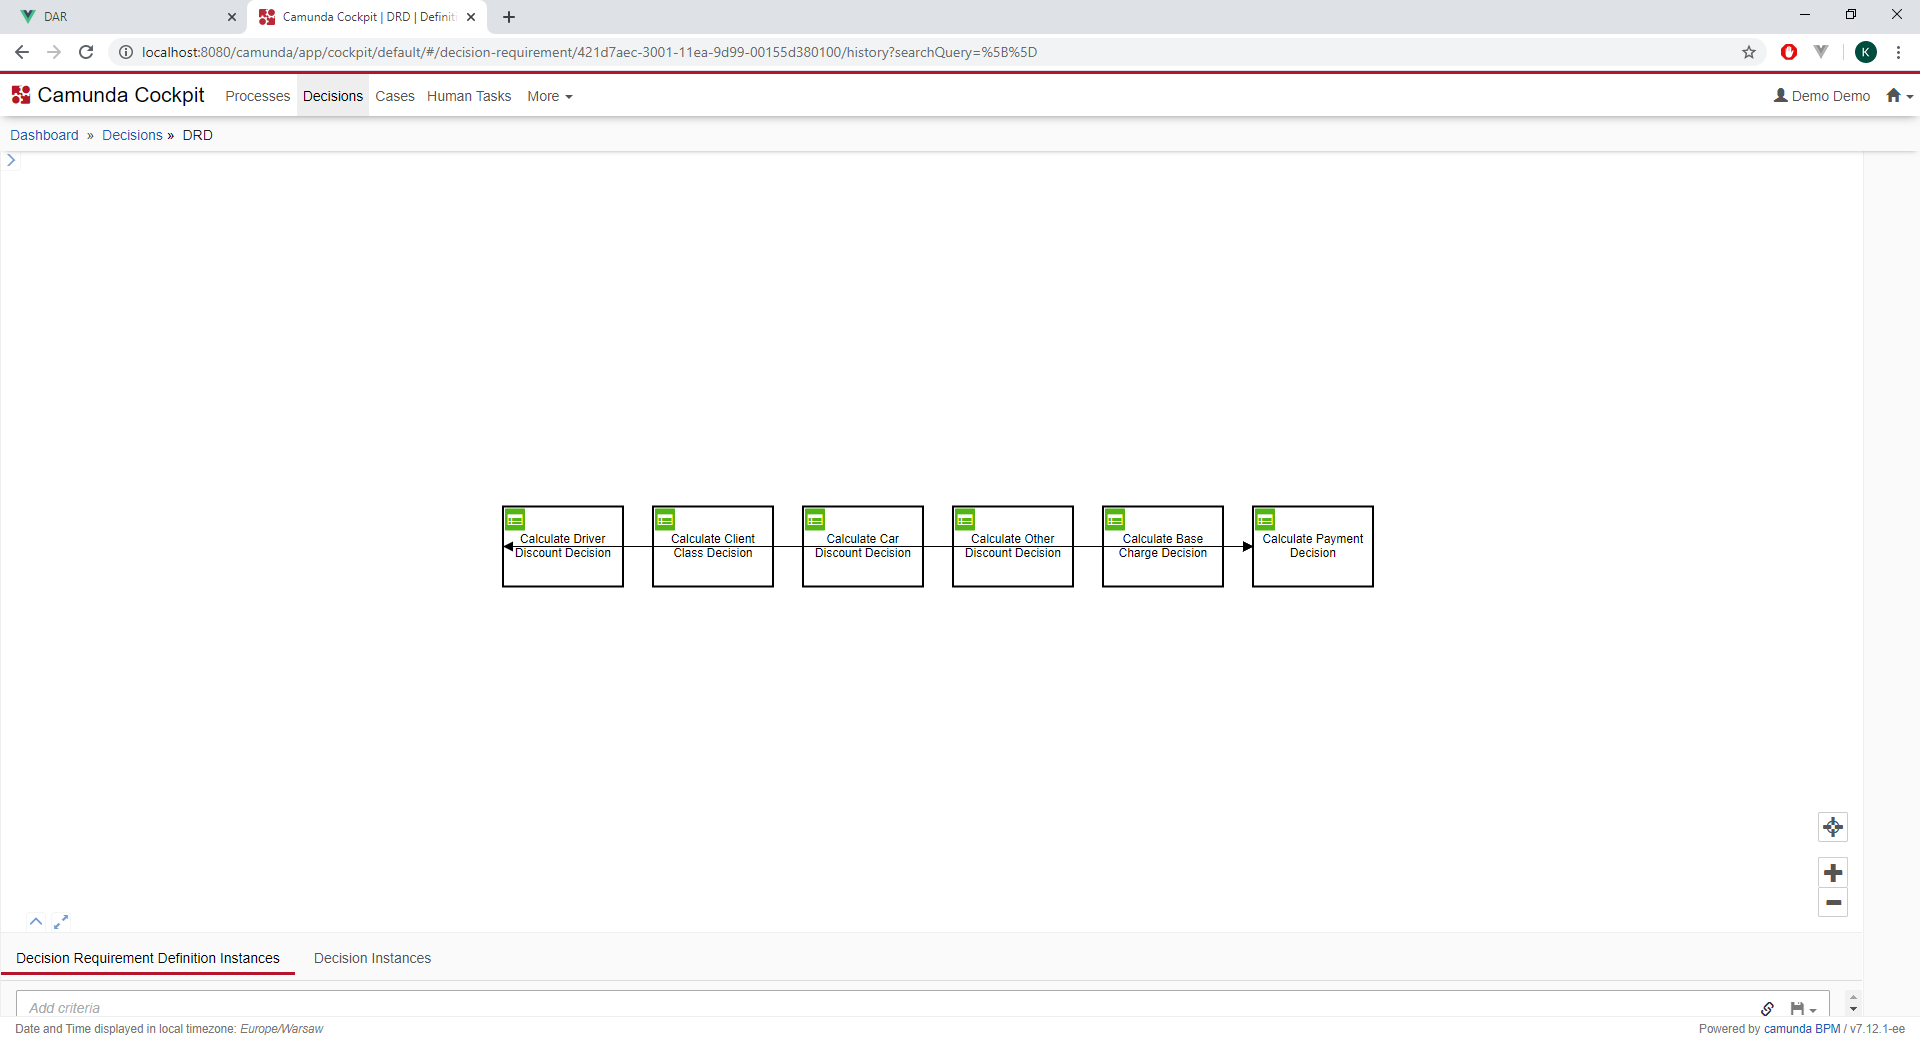
\includegraphics[width=\textwidth]{./assets/camundaExampleDMN.png}
    \caption{Model \emph{DMN} pliku ,,example''}
    \label{fig:camundaExampleDMN}
\end{figure}

Jak już zostało w~pracy nadmienione diagramy \emph{ARD} dostarczają informacje pozwalające na stworzenie modeli \emph{DMN} oraz związanych z~nimi tablic decyzyjnych, w~których określona jest ilość atrybutów wejściowych i~wyjściowych, ich nazwy oraz typy wartości. Reguły biznesowe jednak pozostają puste. Dlatego po wdrożeniu użytkownik musi sam edytować tablice decyzyjne i~według własnego uznania wypełnić reguły. Rysunek~\ref{fig:camundaExampleRules} prezentuje edycję jednej z~tablic decyzyjnych związanych z~jedną z~decyzji z~rysunku~\ref{fig:camundaExampleDMN}. Na potrzeby przykładu dodane zostały dwa wiersze reguł. Każda z~tablic decyzyjnych została w~podobny sposób wypełniona, aby móc uruchomić proces.
\begin{figure}
    \centering
    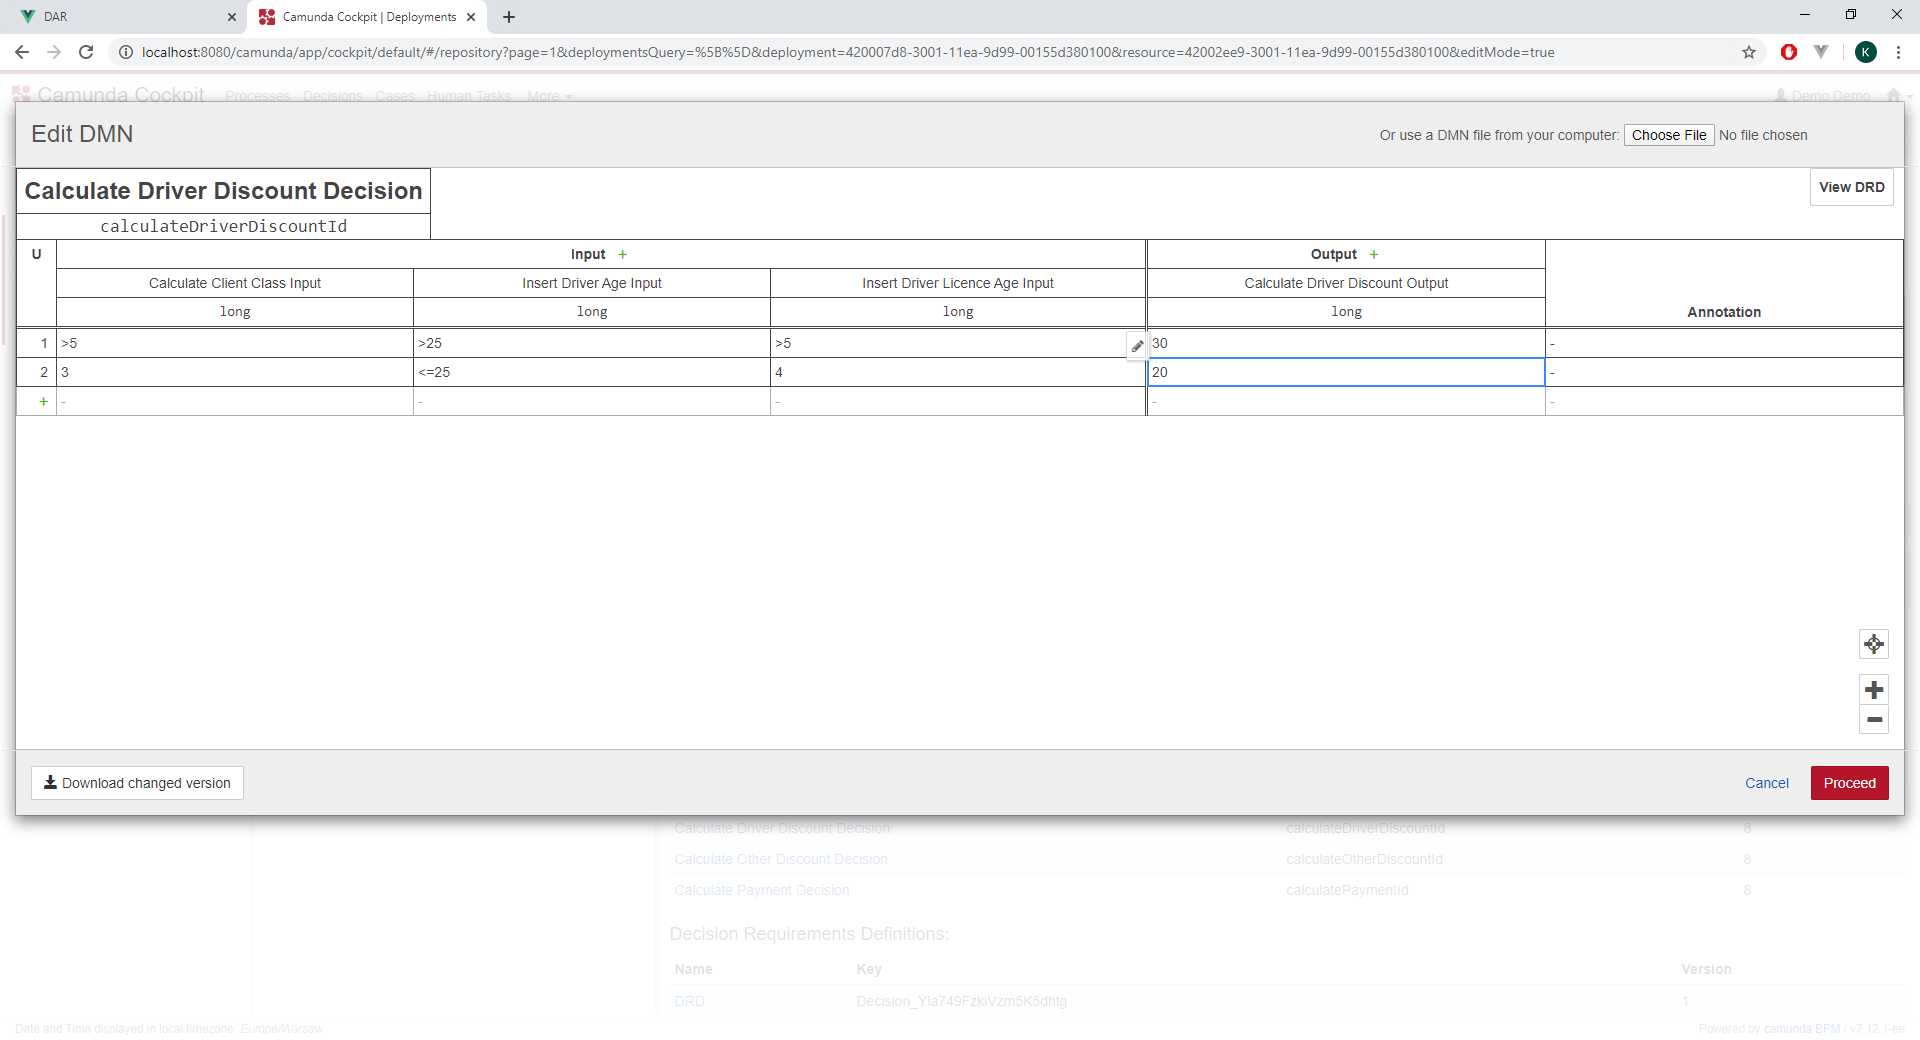
\includegraphics[width=\textwidth]{./assets/camundaExampleRules.png}
    \caption{Edycja tablicy decyzyjnej}
    \label{fig:camundaExampleRules}
\end{figure}

W tym momencie nic nie stoi na przeszkodzie, aby uruchomić proces. Żeby tego dokonać trzeba przejść do \emph{Camunda Tasklist} (używając menu, w~prawym górnym rogu interfejsu w~kształcie domku). Widok z~jakim spotyka się użytkownik jest przedstawiony na rysunku~\ref{fig:camundaTasklistDefault}. Tutaj wyświetlone będą wszystkie zadania wykonywalne przez użytkownika potrzebne do działania procesu, np. zadania związane z~podaniem danych wejściowych. Wyświetlone zadania można odpowiednio filtrować.
\begin{figure}
    \centering
    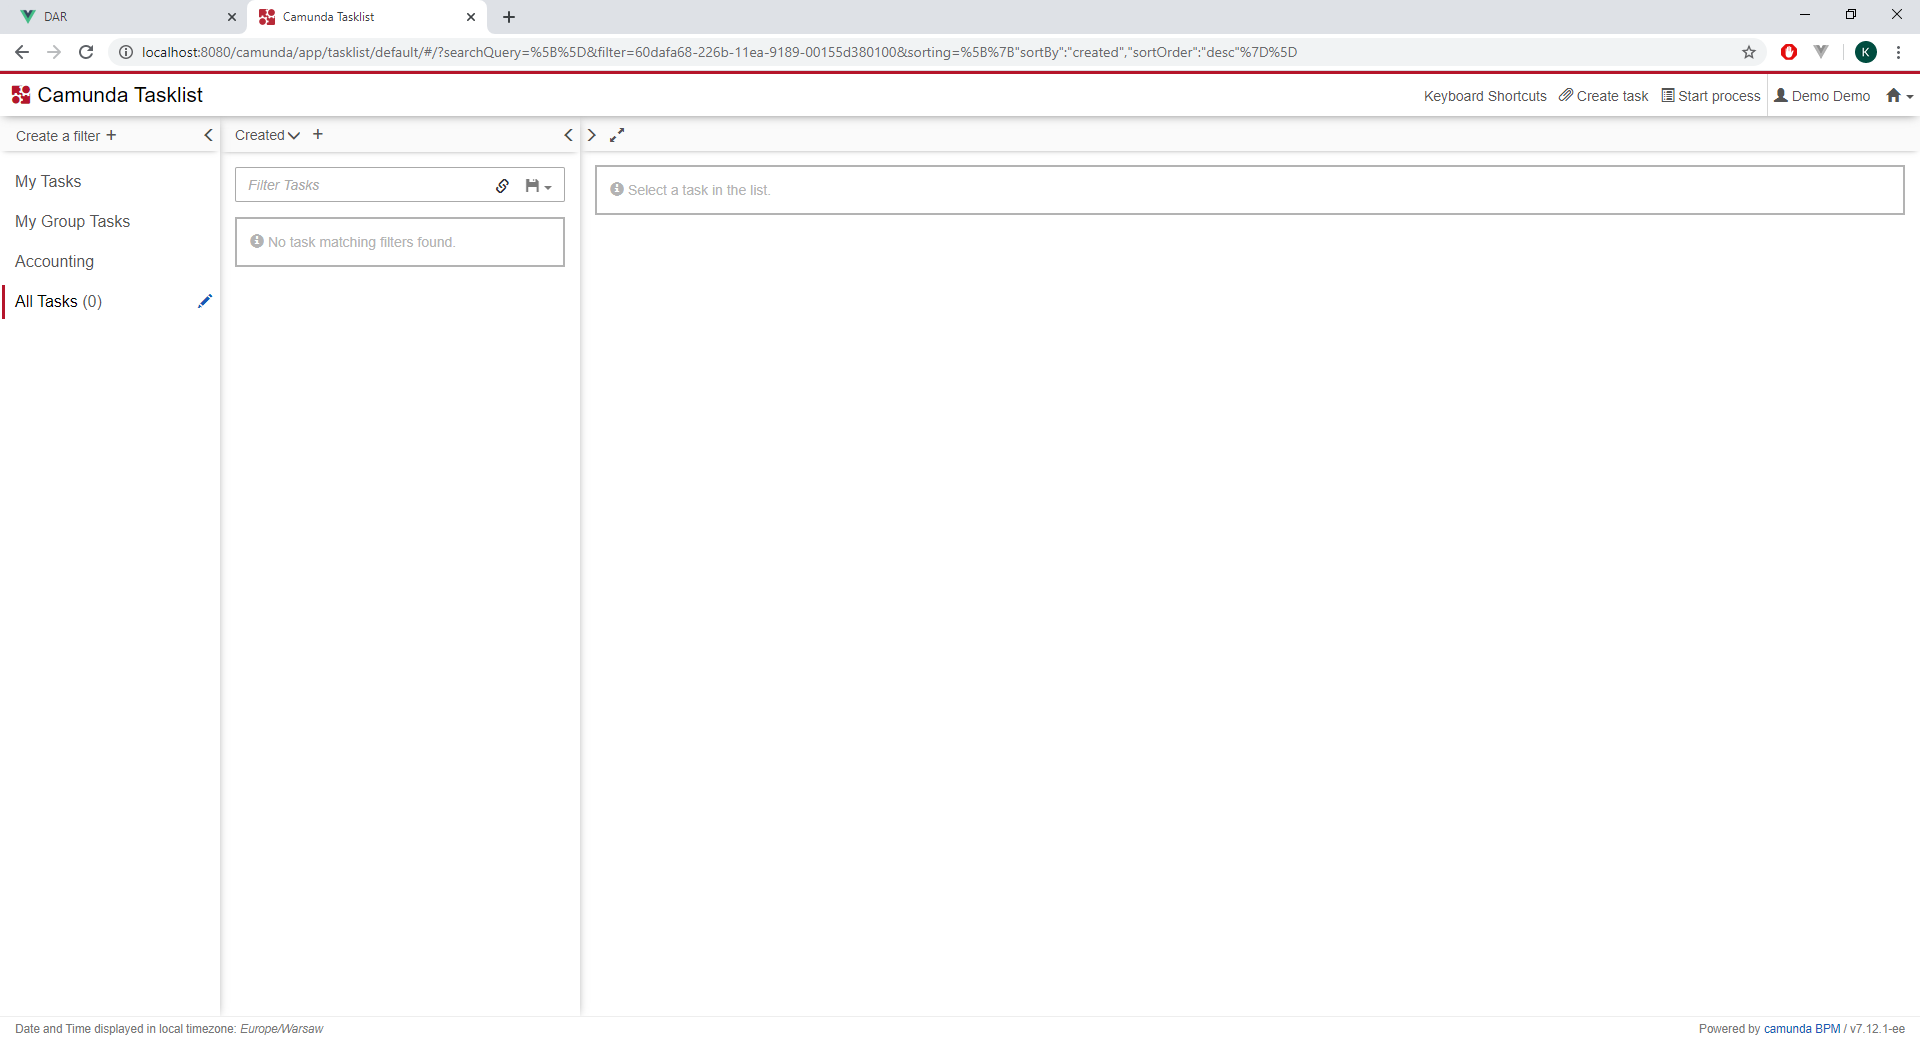
\includegraphics[width=\textwidth]{./assets/camundaTasklistDefault.png}
    \caption{Domyślny ekran \emph{Camunda Tasklist}}
    \label{fig:camundaTasklistDefault}
\end{figure}

Aby uruchomić proces, należy wybrać przycisk ,,Start process'' w~prawym górnym rogu, wybrać odpowiedni model \emph{BPMN} (w~tym przypadku będzie to ,,example''), nadać tej instancji procesu pewien identyfikator, dla przykładu będzie to ,,ExampleBuisnessKey'' i~nacisnąć przycisk ,,Start''. Spowoduje to pojawienie się adnotacji, że proces został uruchomiony. Można w~tym momencie wrócić do modułu \emph{Camunda Cockpit}, gdzie na stronie z~rysunku~\ref{fig:camundaCockpitDefault} w~metrykach nastąpi zmiana -- pokazane zostanie, że pewien proces działa. W zakładce ,,Processes'' wyświetlona będzie instancja procesu, która po naciśnięciu pokaże aktualny stan wykonywania procesu. Jednak przed przejściem do wspomnianego modułu warto odświeżyć \emph{Camunda Tasklist}. Pojawi się lista wykonywalnych zadań związanych z~procesem, który został uruchomiony. Są to dane wejściowe, które musi podać użytkownik, aby proces kontynuować działanie. Rysunek~\ref{fig:camundaTasklistTask} prezentuje opisaną listę oraz wypełnienie jednego z~takich zadań. Na potrzeby przykładu wszystkie zadania zostały wykonane.
\begin{figure}
    \centering
    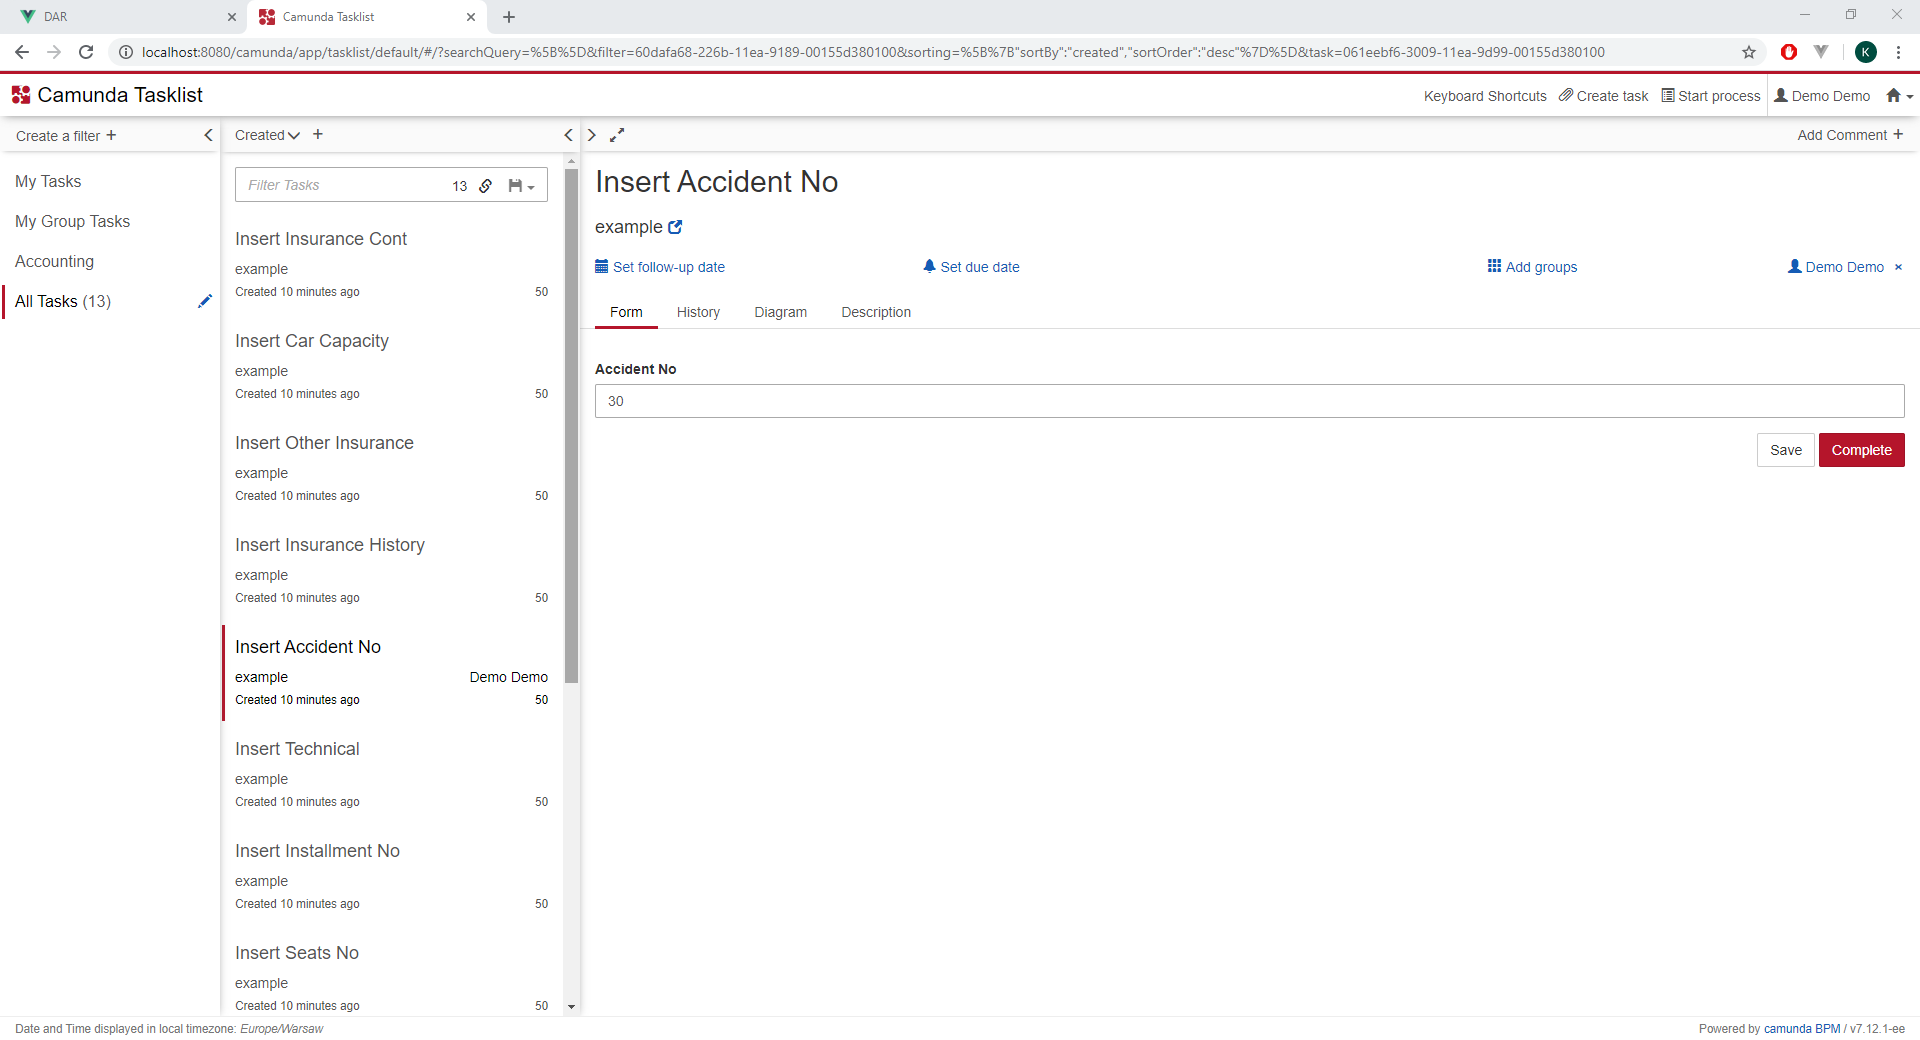
\includegraphics[width=\textwidth]{./assets/camundaTasklistTask.png}
    \caption{Wypełnione \emph{zadanie} wraz z~listą oczekujących zadań}
    \label{fig:camundaTasklistTask}
\end{figure}

Po wykonaniu wszystkich zadań warto przejść do modułu \emph{Camunda Cockpit} do zakładki ,,Processes'', wybrać tam odpowiedni proces i~po wyświetleniu modelu \emph{BPMN} nacisnąć przycisk ,,History''. Opcja ,,Runtime'' w~tym momencie nic nie wyświetla, ponieważ proces został zakończony, wszystkie decyzje zostały zewaluowane, jednak tak jak to było opisywane wcześniej, w~przypadku wykonywania procesu to jest miejsce, gdzie można śledzić działanie procesu. Rysunek~\ref{fig:camundaCockpitCompleted} prezentuje widok ,,History''. 
\begin{figure}
    \centering
    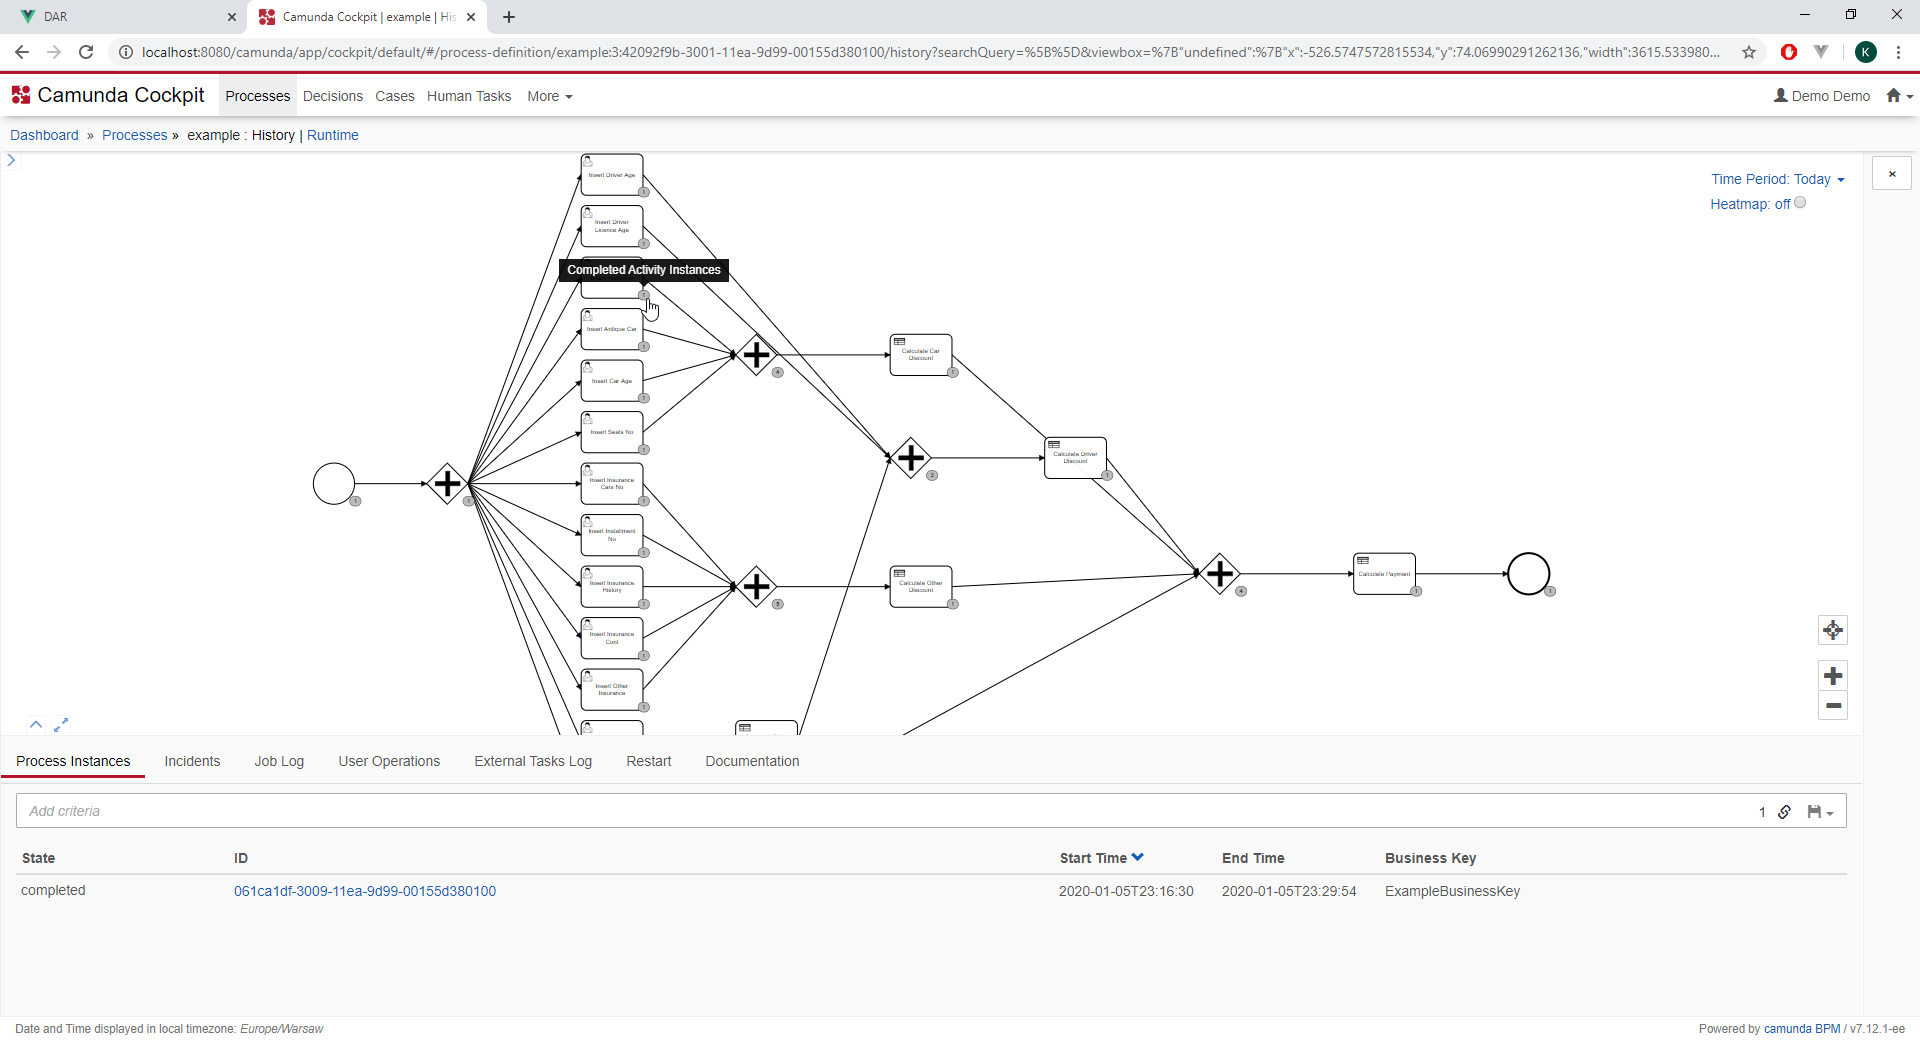
\includegraphics[width=\textwidth]{./assets/camundaCockpitCompleted.png}
    \caption{Historia wykonywania procesu}
    \label{fig:camundaCockpitCompleted}
\end{figure}
Dodatkowo można w~tym miejscu sprawdzić jak rozkładała się praca procesu, aby ewentualnie go usprawniać. Rysunek~\ref{fig:camundaCockpitHeat} przedstawia przydatny do tego widok.
\begin{figure}
    \centering
    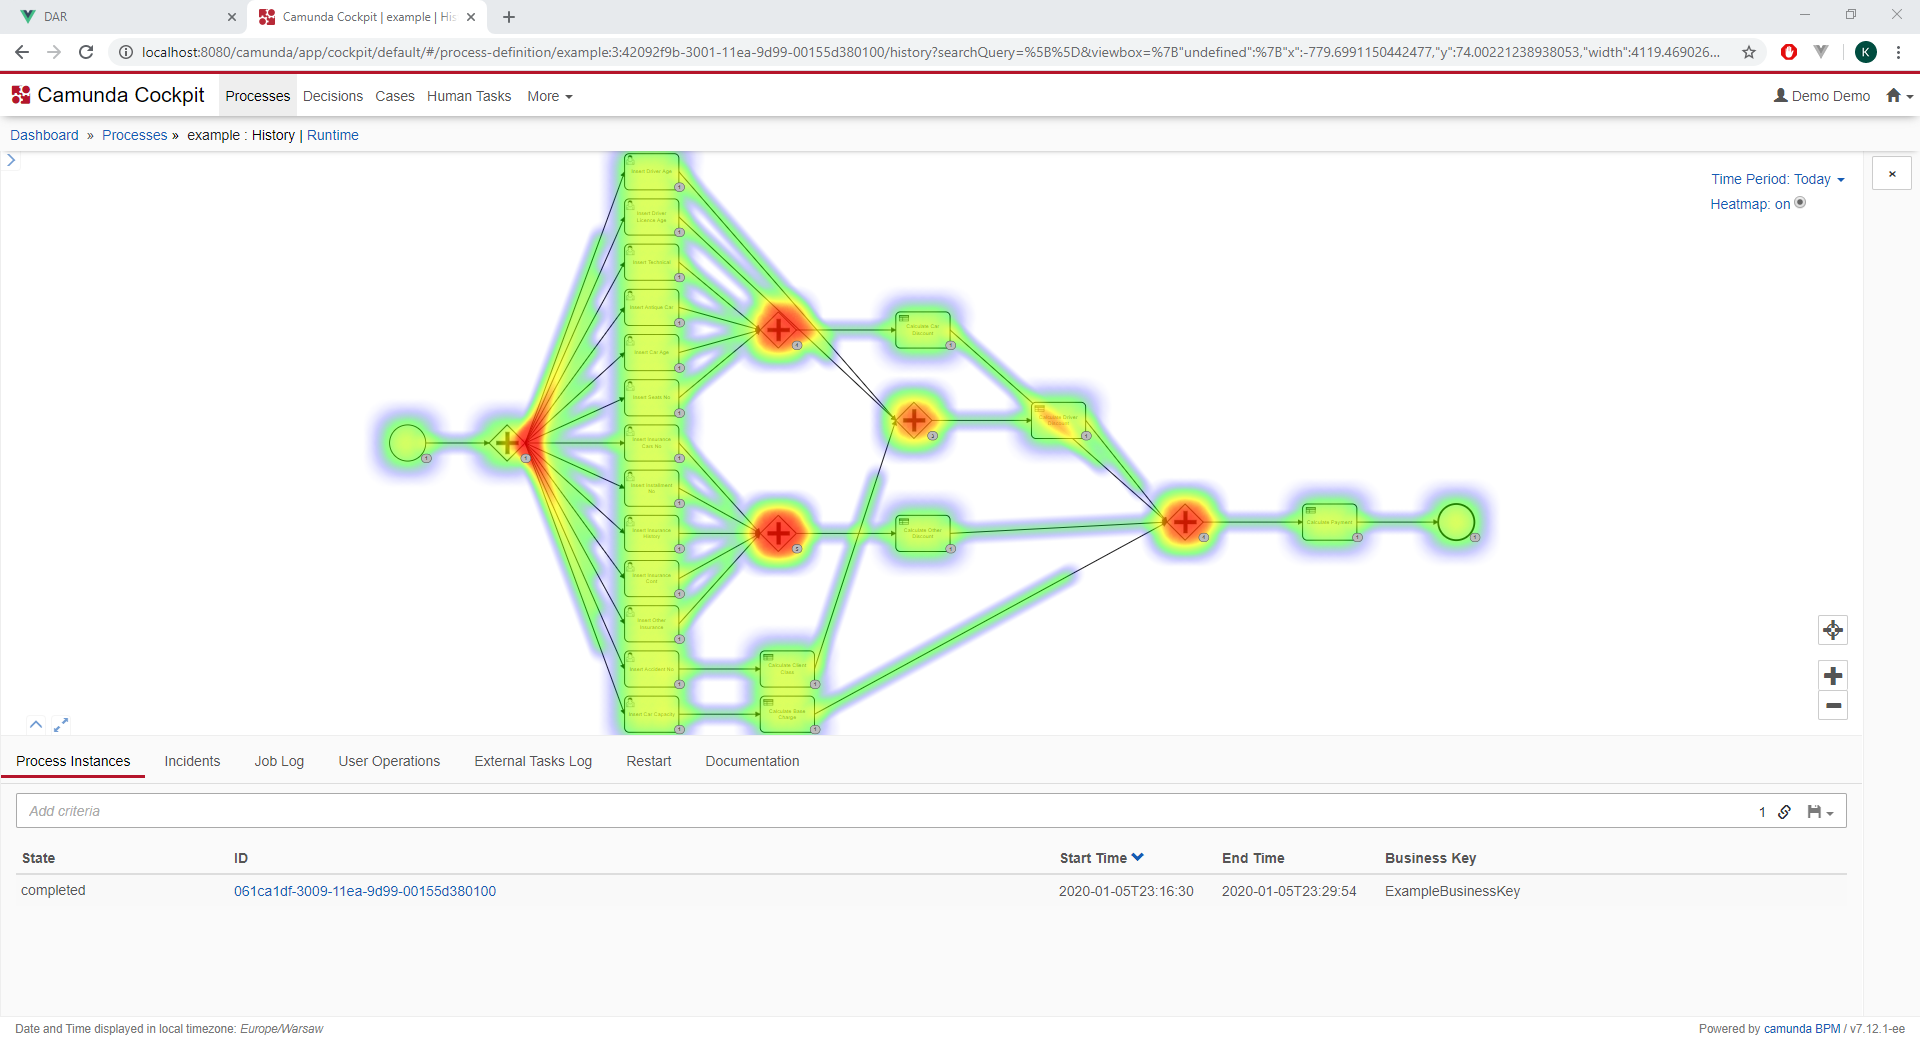
\includegraphics[width=\textwidth]{./assets/camundaCockpitHeat.png}
    \caption{Rozkład pracy procesu}
    \label{fig:camundaCockpitHeat}
\end{figure} 

W dolnej części rysunku~\ref{fig:camundaCockpitCompleted} widać instancję zakończonego procesu. Po naciśnięciu ,,ID'' tej instancji, widok modelu zostaje ten sam, jednak dochodzi wiele zakładek związanych z~historią wykonywania tego procesu, np. jakie zadania zostały wykonane, jakie były wartości danych i~jakie decyzje zostały ewaluowane. Aby zobaczyć wynik końcowy wystarczy przejść do ewaluowanych decyzji i~wybrać finalną decyzję, czyli w~prezentowanym przykładzie ,,Calculate Payment''. Po wybraniu tej decyzji zostaje tylko przejść do jej instancji. Rysunek~\ref{fig:camundaCockpitFinal} przedstawia wynik całego procesu i~jakie były finalne wartości atrybutów -- koszt ubezpieczenia w~tym przypadku wyniósł 100 PLN. Oczywiście w~ramach przykładu reguły są trywialne, w~przedstawionej tablicy decyzyjnej występuje tylko jeden wiersz reguł, jednak w~prawdziwym świecie może ich być dowolna liczba.
\begin{figure}
    \centering
    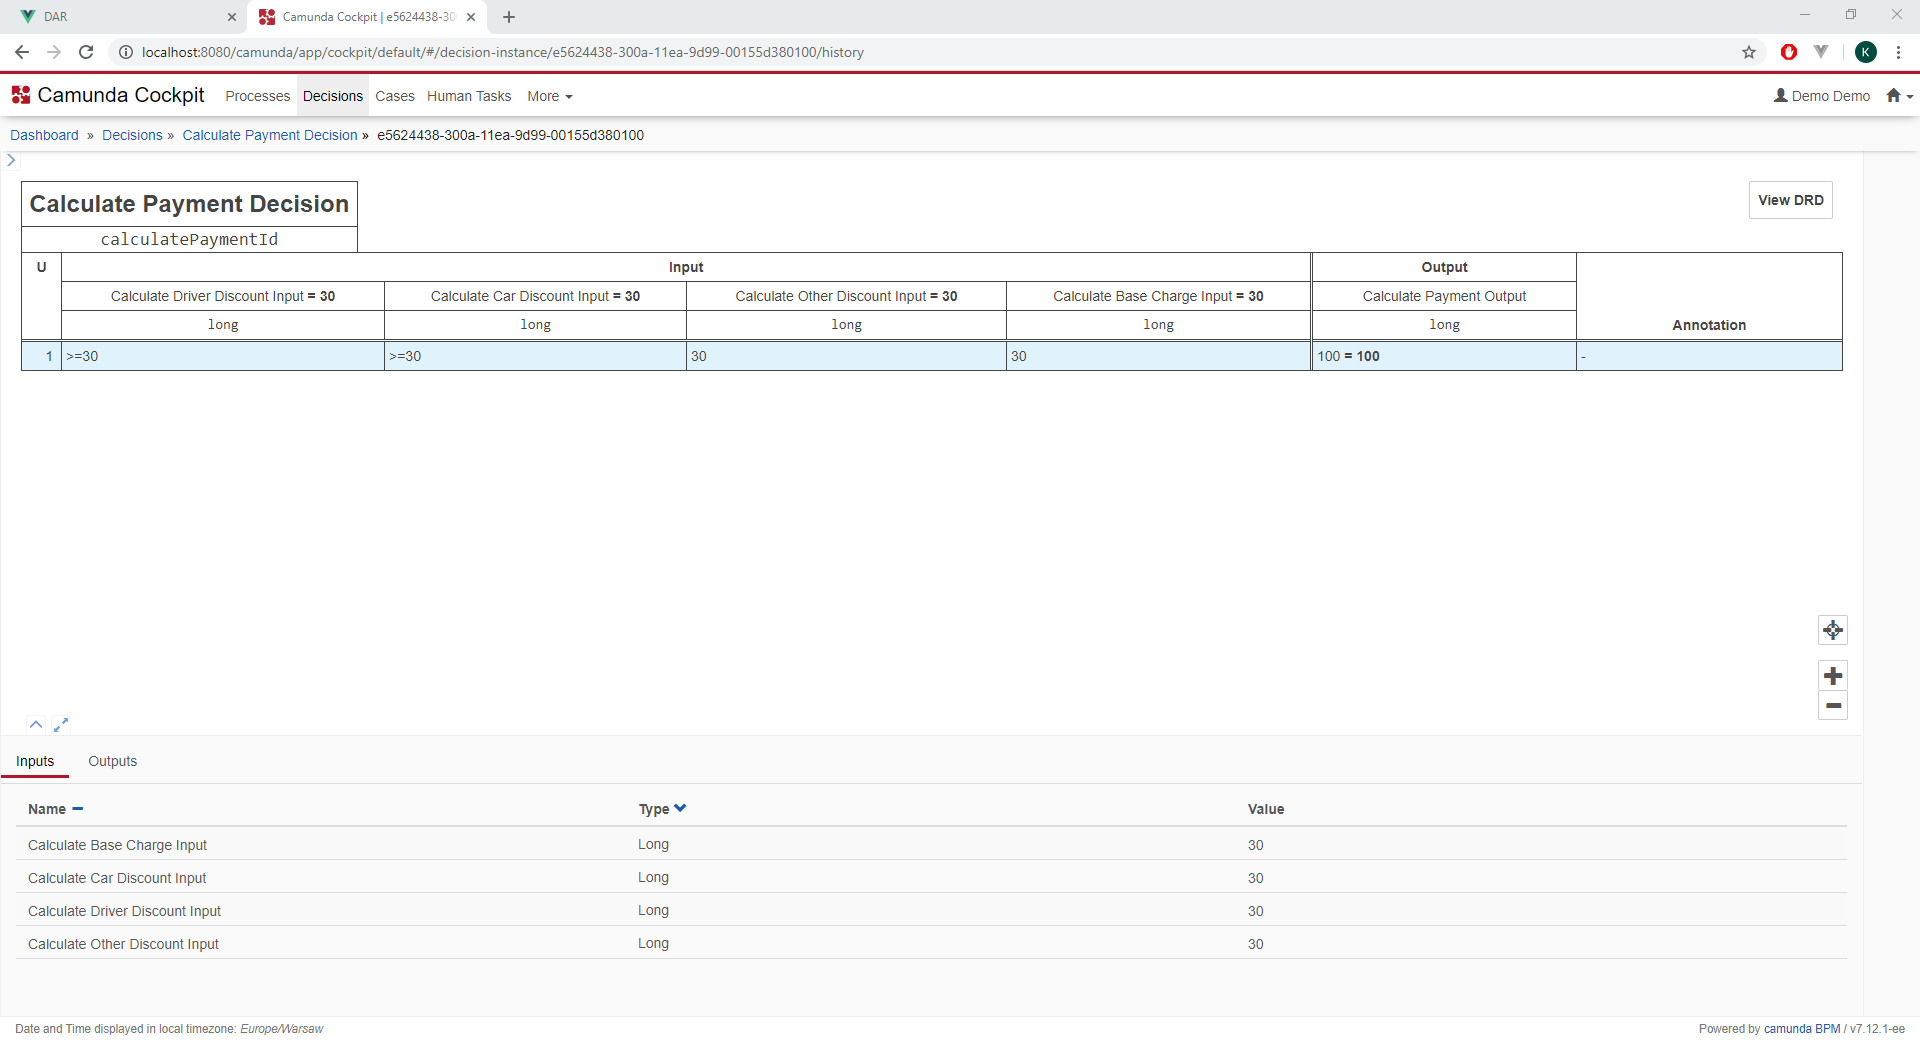
\includegraphics[width=\textwidth]{./assets/camundaCockpitFinal.png}
    \caption{Wynik procesu}
    \label{fig:camundaCockpitFinal}
\end{figure}
\vspace{-6mm}
%---------------------------------------------------------------------------
\section{Podsumowanie wyników}
\label{sec:podsumowanieWyników}
Aplikacja spełnia wszystkie założone wymagania. Generowane modele w~notacji \emph{BPMN} oraz \emph{DMN} poprawnie opisują diagram \emph{ARD} zapisany w~podanym pliku \emph{HML}. Interfejs aplikacji ,,DAR`` jest intuicyjny i~przejrzysty. Kod aplikacji w~większości jest asynchroniczny co sprawia, że aplikacja jest płynniejsza w~działaniu. Zintegrowany system \emph{Camunda} poprawnie uruchamia wdrożone procesy. W~przypadku decyzji, ewaluacja również jest poprawna, wymogiem jest tylko uzupełnienie reguł przez użytkownika. Sam wynik końcowy jest zadowalający i~zgodny z~oczekiwaniami.
\vspace{4mm}

Jest to koniec rozdziału przedstawiającego działanie aplikacji. W tym rozdziale przedstawione zostały najważniejsze funkcjonalności systemu na konkretnym przykładzie. W kolejnym, końcowym rozdziale przedstawione zostaną wnioski nasuwające się po zapoznaniu się z~aplikacją oraz możliwe kierunki rozwoju aplikacji. 



\chapter{Podsumowanie}
\label{cha:podsumowanie}
Rozdział kończy niniejszą pracę podsumowując działanie systemu oraz opisując zebrane wnioski. Dodatkowo przedstawia możliwe kierunki rozwoju aplikacji.

%---------------------------------------------------------------------------
\section{Wnioski}
\label{sec:wnioski}
W ramach niniejszej pracy został osiągnięty cel, jakim było zaprojektowanie i~zaimplementowanie aplikacji internetowej, będącej generatorem modeli w~notacji \emph{BPMN} oraz \emph{DMN} na bazie plików \emph{HML}, opisujących diagramy \emph{ARD} oraz integrację z~zewnętrznym systemem wspierającym zarządzanie procesami biznesowymi oraz ewaluację decyzji.

Praca całościowo opisuje proces tworzenia aplikacji ,,DAR``, wprowadzając najpierw najważniejsze pojęcia używane w~pracy, by następnie przedstawić projekt aplikacji z~odpowiednimi schematami i~jego implementację wraz z~opisem wykorzystanych technologii. Finalnie praca prezentuje przebieg działania aplikacji na konkretnym przykładzie, pokazując dokładnie interfejs użytkownika.

W projekcie wymagające dodatkowej implementacji okazało się tworzenie modeli \emph{BPMN} oraz \emph{DMN}, wszystko za sprawą nieaktualnych bibliotek do modelowania obiektów \emph{BPMN} oraz \emph{DMN} w~środowisku \emph{.NET}. Zadaniem prostym w~implementacji było stworzenie odpowiednich definicji zadań lub przejść, jednak tworzenie na tej podstawie konkretnych obiektów na diagramie okazało się być wymagające. Sam algorytm do wyciągania informacji z~pliku \emph{HML} i~odpowiednia transformacja informacji z~diagramu \emph{ARD} do \emph{BPMN} był tworzony głównie z~myślą o wydajności, mając na uwadze fakt, że w~jednej chwili może być obsługiwanych wiele plików \emph{HML}. Integracja z~systemem \emph{Camunda} również przysporzyła wiele problemów, ponieważ wymagała ona modyfikacji modeli \emph{BPMN} oraz \emph{DMN} o specyficzne dla tego systemu adnotacje i~informacje w~plikach wdrażanych na ten system. Organizacja tworząca system \emph{Camunda} zakłada, że wszystkie modele wdrażane na platformę \emph{Camunda} będą tworzone przez jej autorski edytor modeli. Ten edytor modeli nie udostępnia jednak \emph{API}, dlatego zaszła potrzeba modyfikacji zaimplementowanych w~aplikacji ,,DAR`` edytorów modeli, aby były zgodne ze standardem \emph{Camunda}. Największym wyzwaniem było odkrycie tego problemu, ponieważ \emph{API} wystawione przez \emph{Camunda} służące do wdrożeń modeli nie zwracało żadnych konkretnych błędów.
\newpage

%---------------------------------------------------------------------------
\section{Możliwe kierunki rozwoju aplikacji}
\label{sec:rozwójAplikacji}
Główną możliwością rozwoju aplikacji jest wzbogacenie procesu związanego z~tworzenia modeli \emph{BPMN} oraz \emph{DMN}. W tym momencie wszystkie proste, niezależne własności z~diagramu \emph{ARD}, które potrzebne są jako dane wejściowe są umieszczane na samym początku modelu \emph{BPMN} i~dla każdego z~nich przypisana jest jedna aktywność wykonywalna. Podobnie w~przypadku skomplikowanych, zależnych własności -- do każdej jednej takiej własności przypisana jest jedna decyzja z~modelu \emph{DMN}. Jest to przypadek głębokości poziomu zero (poziomy głębokości wytłumaczone są w~pracy~\cite{ARDtoBPM}). Warto byłoby wprowadzić możliwość wyboru poziomu głębokości, aby proste niezależne własności były łączone w~grupy o wielkości zależnej od głębokości i~każdej takiej grupie byłyby przyporządkowywane odpowiednie zadania wykonywalne. Na tej samej zasadzie decyzje w~zależności od poziomu głębokości mogą odpowiadać nie jednej skomplikowanej, zależnej własności, a~przykładowo pewnej grupie. 

Drugim z~możliwych kierunków rozwoju jest wprowadzenie reguł decyzyjnych dla tablic decyzyjnych w~modelu \emph{DMN}. Gdyby plik \emph{HML} rozszerzyć o takie reguły, aby mogły być one odpowiednio wydobyte i~wdrożone do modelu \emph{DMN} lub gdyby dostarczyć jakieś źródło takich reguł, tak aby użytkownik nie musiał ręcznie ich uzupełniać po wdrożeniu procesu, zaimplementowane rozwiązanie byłoby w~pełni zautomatyzowane.

Pomysłem wartym rozważenia jest również rozbudowa aplikacji o wsparcie generacji modeli \emph{ARD}. W tym momencie aplikacja potrafi przetwarzać pliki \emph{HML}, opisujące diagram \emph{ARD}, jednak nie jest w~stanie użytkownikowi pokazać, jak taki diagram wygląda.

Kolejną sprawą jest część \emph{TPH} w~pliku \emph{HML}. Zapisane w tej części informacje mogłyby być wykorzystane, tak jak w przypadku z poprzedniego akapitu, do zwrócenia diagramu \emph{TPH}, aby użytkownik mógł go fizycznie zobaczyć. Dodatkowo wykorzystanie diagramów \emph{TPH} pozwoliłoby ulepszyć tworzone modele \emph{BPMN} oraz \emph{DMN}.

Patrząc bardziej od strony technicznej -- pierwszą rzeczą jest brak rozwiązania chmurowego. W tym momencie cała aplikacja jest uruchamiana lokalnie, potrzebny jest fizyczny komputer użytkownika wraz z~serwerem bazy danych i~trzema wolnymi portami odpowiednio dla aplikacji klienckiej, serwera ,,DAR'' oraz serwera \emph{Camunda}. Prostym rozwiązaniem jest wdrożenie całej aplikacji na chmurę. Dodatkowo dobrym pomysłem jest konteneryzacja systemu, szczególnie w~przypadku gdy szkielet aplikacyjny \emph{ASP .NET Core} jest bardzo dobrze przystosowany do konteneryzacji. To samo tyczy się aplikacji klienckiej. 

Finalnie możliwą zmianą jest zastąpienie systemu \emph{Camunda} przez własną aplikację. Oczywiście byłoby to bardzo duże przedsięwzięcie, wymagające własnej implementacji silników procesowych i~decyzyjnych oraz całej logiki z~wykonywaniem procesów, a~także odpowiednim prezentowaniu działań, z~wyświetlaniem diagramów \emph{BPMN} oraz \emph{DMN} na czele.

\printbibliography

\end{document}
